% -----------------------------------------------------------------------------
%                                     HEADER                                    
% -----------------------------------------------------------------------------
\documentclass[a4paper, 10pt]{article}
\usepackage{jheppub}
\usepackage[T1]{fontenc}
\usepackage{colortbl,xcolor,float}
\definecolor{orange}{rgb}{1,0.5,0}
% -----------------------------------------------------------------------------
%                                   COVER PAGE                                  
% -----------------------------------------------------------------------------
\title{{
\includegraphics[scale=.4]{logo.eps}}\ The LaTeX report}

\author{Generated by elijahsheridan on 25 March 2020, 17:09:37}

\abstract{
  This report has been generated automatically
  by {\sc MadAnalysis} 5.\\$~$\\ 
  Please cite:\\ 
  \begin{quote}
    \textbf{E.~Conte, B.~Fuks and G.~Serret},\\ 
    \textit{MadAnalysis 5, A User-Friendly
    Framework for Collider Phenomenology},\\ 
    Comput. Phys. Commun. {\bf 184} (2013) 222-256,\\
    arXiv:1206.1599 [hep-ph].\\ 
  \end{quote}
  To contact us:\\ 
  \begin{quote}
    \textbf{http://madanalysis.irmp.ucl.ac.be}\\
    \textbf{ma5team@iphc.cnrs.fr}\\
  \end{quote}
}

% -----------------------------------------------------------------------------
%                                 BEGIN DOCUMENT                                
% -----------------------------------------------------------------------------
\begin{document}
\maketitle
\flushbottom

% -----------------------------------------------------------------------------
%                                 SECTION Setup                                 
% -----------------------------------------------------------------------------
\newpage
\section{ Setup}

\subsection{ Command history}

\texttt{ma5>\# set directory where running "./\-bin/\-ma5"; set lumi; define the signal significance\\
}
\texttt{ }\texttt{ }\texttt{ma5>set main.currentdir = /\-Users/\-elijahsheridan/\-MG5\_aMC\_v2\_6\_5/\-axion\_pheno \# need to change this directory path --> exit and type "pwd" to get the path\\
}
\texttt{ }\texttt{ }\texttt{ma5>set main.lumi = 40.0\\
}
\texttt{ }\texttt{ }\texttt{ma5>set main.SBratio = 'S/\-sqrt(S+B)'\\
}
\texttt{ }\texttt{ }\texttt{ma5>\# import samples --> change the path to the LHE file\\
}
\texttt{ }\texttt{ }\texttt{ma5>import /\-Users/\-elijahsheridan/\-MG5\_aMC\_v2\_6\_5/\-axion\_pheno/\-madgraph\_data/\-axion\_signal/\-axion\_signal\_gurrola\_cuts\_1MeV.lhe.gz as signal\\
}
\texttt{ }\texttt{ }\texttt{ma5>import /\-Users/\-elijahsheridan/\-MG5\_aMC\_v2\_6\_5/\-axion\_pheno/\-madgraph\_data/\-vbf\_diphoton\_background\_data/\-merged\_lhe/\-vbf\_diphoton\_background\_ht\_0\_100\_merged.lhe.gz as bg\_vbf\_0\_100\\
}
\texttt{ }\texttt{ }\texttt{ma5>import /\-Users/\-elijahsheridan/\-MG5\_aMC\_v2\_6\_5/\-axion\_pheno/\-madgraph\_data/\-vbf\_diphoton\_background\_data/\-merged\_lhe/\-vbf\_diphoton\_background\_ht\_100\_200\_merged.lhe.gz as bg\_vbf\_100\_200\\
}
\texttt{ }\texttt{ }\texttt{ma5>import /\-Users/\-elijahsheridan/\-MG5\_aMC\_v2\_6\_5/\-axion\_pheno/\-madgraph\_data/\-vbf\_diphoton\_background\_data/\-merged\_lhe/\-vbf\_diphoton\_background\_ht\_200\_400\_merged.lhe.gz as bg\_vbf\_200\_400\\
}
\texttt{ }\texttt{ }\texttt{ma5>import /\-Users/\-elijahsheridan/\-MG5\_aMC\_v2\_6\_5/\-axion\_pheno/\-madgraph\_data/\-vbf\_diphoton\_background\_data/\-merged\_lhe/\-vbf\_diphoton\_background\_ht\_400\_600\_merged.lhe.gz as bg\_vbf\_400\_600\\
}
\texttt{ }\texttt{ }\texttt{ma5>import /\-Users/\-elijahsheridan/\-MG5\_aMC\_v2\_6\_5/\-axion\_pheno/\-madgraph\_data/\-vbf\_diphoton\_background\_data/\-merged\_lhe/\-vbf\_diphoton\_background\_ht\_600\_800\_merged.lhe.gz as bg\_vbf\_600\_800\\
}
\texttt{ }\texttt{ }\texttt{ma5>import /\-Users/\-elijahsheridan/\-MG5\_aMC\_v2\_6\_5/\-axion\_pheno/\-madgraph\_data/\-vbf\_diphoton\_background\_data/\-merged\_lhe/\-vbf\_diphoton\_background\_ht\_800\_1200\_merged.lhe.gz as bg\_vbf\_800\_1200\\
}
\texttt{ }\texttt{ }\texttt{ma5>import /\-Users/\-elijahsheridan/\-MG5\_aMC\_v2\_6\_5/\-axion\_pheno/\-madgraph\_data/\-vbf\_diphoton\_background\_data/\-merged\_lhe/\-vbf\_diphoton\_background\_ht\_1200\_1600\_merged.lhe.gz as bg\_vbf\_1200\_1600\\
}
\texttt{ }\texttt{ }\texttt{ma5>import /\-Users/\-elijahsheridan/\-MG5\_aMC\_v2\_6\_5/\-axion\_pheno/\-madgraph\_data/\-vbf\_diphoton\_background\_data/\-merged\_lhe/\-vbf\_diphoton\_background\_ht\_1600\_inf\_merged.lhe.gz as bg\_vbf\_1600\_inf\\
}
\texttt{ }\texttt{ }\texttt{ma5>import /\-Users/\-elijahsheridan/\-MG5\_aMC\_v2\_6\_5/\-axion\_pheno/\-madgraph\_data/\-diphoton\_double\_isr\_background\_data/\-merged\_lhe/\-diphoton\_double\_isr\_background\_ht\_0\_100\_merged.lhe.gz as bg\_dip\_0\_100\\
}
\texttt{ }\texttt{ }\texttt{ma5>import /\-Users/\-elijahsheridan/\-MG5\_aMC\_v2\_6\_5/\-axion\_pheno/\-madgraph\_data/\-diphoton\_double\_isr\_background\_data/\-merged\_lhe/\-diphoton\_double\_isr\_background\_ht\_100\_200\_merged.lhe.gz as bg\_dip\_100\_200\\
}
\texttt{ }\texttt{ }\texttt{ma5>import /\-Users/\-elijahsheridan/\-MG5\_aMC\_v2\_6\_5/\-axion\_pheno/\-madgraph\_data/\-diphoton\_double\_isr\_background\_data/\-merged\_lhe/\-diphoton\_double\_isr\_background\_ht\_200\_400\_merged.lhe.gz as bg\_dip\_200\_400\\
}
\texttt{ }\texttt{ }\texttt{ma5>import /\-Users/\-elijahsheridan/\-MG5\_aMC\_v2\_6\_5/\-axion\_pheno/\-madgraph\_data/\-diphoton\_double\_isr\_background\_data/\-merged\_lhe/\-diphoton\_double\_isr\_background\_ht\_400\_600\_merged.lhe.gz as bg\_dip\_400\_600\\
}
\texttt{ }\texttt{ }\texttt{ma5>import /\-Users/\-elijahsheridan/\-MG5\_aMC\_v2\_6\_5/\-axion\_pheno/\-madgraph\_data/\-diphoton\_double\_isr\_background\_data/\-merged\_lhe/\-diphoton\_double\_isr\_background\_ht\_600\_800\_merged.lhe.gz as bg\_dip\_600\_800\\
}
\texttt{ }\texttt{ }\texttt{ma5>import /\-Users/\-elijahsheridan/\-MG5\_aMC\_v2\_6\_5/\-axion\_pheno/\-madgraph\_data/\-diphoton\_double\_isr\_background\_data/\-merged\_lhe/\-diphoton\_double\_isr\_background\_ht\_800\_1200\_merged.lhe.gz as bg\_dip\_800\_1200\\
}
\texttt{ }\texttt{ }\texttt{ma5>import /\-Users/\-elijahsheridan/\-MG5\_aMC\_v2\_6\_5/\-axion\_pheno/\-madgraph\_data/\-diphoton\_double\_isr\_background\_data/\-merged\_lhe/\-diphoton\_double\_isr\_background\_ht\_1200\_1600\_merged.lhe.gz as bg\_dip\_1200\_1600\\
}
\texttt{ }\texttt{ }\texttt{ma5>import /\-Users/\-elijahsheridan/\-MG5\_aMC\_v2\_6\_5/\-axion\_pheno/\-madgraph\_data/\-diphoton\_double\_isr\_background\_data/\-merged\_lhe/\-diphoton\_double\_isr\_background\_ht\_1600\_inf\_merged.lhe.gz as bg\_dip\_1600\_inf\\
}
\texttt{ }\texttt{ }\texttt{ma5>\# define bg and signal samples\\
}
\texttt{ }\texttt{ }\texttt{ma5>set signal.type = signal\\
}
\texttt{ }\texttt{ }\texttt{ma5>set bg\_vbf\_0\_100.type = background\\
}
\texttt{ }\texttt{ }\texttt{ma5>set bg\_vbf\_100\_200.type = background\\
}
\texttt{ }\texttt{ }\texttt{ma5>set bg\_vbf\_200\_400.type  = background\\
}
\texttt{ }\texttt{ }\texttt{ma5>set bg\_vbf\_400\_600.type  = background\\
}
\texttt{ }\texttt{ }\texttt{ma5>set bg\_vbf\_600\_800.type  = background\\
}
\texttt{ }\texttt{ }\texttt{ma5>set bg\_vbf\_800\_1200.type  = background\\
}
\texttt{ }\texttt{ }\texttt{ma5>set bg\_vbf\_1200\_1600.type  = background\\
}
\texttt{ }\texttt{ }\texttt{ma5>set bg\_vbf\_1600\_inf.type = background\\
}
\texttt{ }\texttt{ }\texttt{ma5>set bg\_dip\_0\_100.type = background\\
}
\texttt{ }\texttt{ }\texttt{ma5>set bg\_dip\_100\_200.type = background\\
}
\texttt{ }\texttt{ }\texttt{ma5>set bg\_dip\_200\_400.type = background\\
}
\texttt{ }\texttt{ }\texttt{ma5>set bg\_dip\_400\_600.type = background\\
}
\texttt{ }\texttt{ }\texttt{ma5>set bg\_dip\_600\_800.type = background\\
}
\texttt{ }\texttt{ }\texttt{ma5>set bg\_dip\_800\_1200.type = background\\
}
\texttt{ }\texttt{ }\texttt{ma5>set bg\_dip\_1200\_1600.type = background\\
}
\texttt{ }\texttt{ }\texttt{ma5>set bg\_dip\_1600\_inf.type = background\\
}
\texttt{ }\texttt{ }\texttt{ma5>\# define weights for the samples\\
}
\texttt{ }\texttt{ }\texttt{ma5>\#set sample\_1.weight = 1\\
}
\texttt{ }\texttt{ }\texttt{ma5>\#set sample\_2.weight = 1\\
}
\texttt{ }\texttt{ }\texttt{ma5>\# line styles and colors\\
}
\texttt{ }\texttt{ }\texttt{ma5>set signal.linecolor = red\\
}
\texttt{ }\texttt{ }\texttt{ma5>set signal.linestyle = dashed\\
}
\texttt{ }\texttt{ }\texttt{ma5>set signal.linewidth = 3\\
}
\texttt{ }\texttt{ }\texttt{ma5>set bg\_vbf\_0\_100.linecolor = blue-4\\
}
\texttt{ }\texttt{ }\texttt{ma5>set bg\_vbf\_0\_100.linestyle = dash-dotted\\
}
\texttt{ }\texttt{ }\texttt{ma5>set bg\_vbf\_0\_100.linewidth = 4\\
}
\texttt{ }\texttt{ }\texttt{ma5>set bg\_vbf\_100\_200.linecolor = blue-3\\
}
\texttt{ }\texttt{ }\texttt{ma5>set bg\_vbf\_100\_200.linestyle = dash-dotted\\
}
\texttt{ }\texttt{ }\texttt{ma5>set bg\_vbf\_100\_200.linewidth = 4\\
}
\texttt{ }\texttt{ }\texttt{ma5>set bg\_vbf\_200\_400.linecolor = blue-2\\
}
\texttt{ }\texttt{ }\texttt{ma5>set bg\_vbf\_200\_400.linestyle = dash-dotted\\
}
\texttt{ }\texttt{ }\texttt{ma5>set bg\_vbf\_200\_400.linewidth = 4\\
}
\texttt{ }\texttt{ }\texttt{ma5>set bg\_vbf\_400\_600.linecolor = blue-1\\
}
\texttt{ }\texttt{ }\texttt{ma5>set bg\_vbf\_400\_600.linestyle = dash-dotted\\
}
\texttt{ }\texttt{ }\texttt{ma5>set bg\_vbf\_400\_600.linewidth = 4\\
}
\texttt{ }\texttt{ }\texttt{ma5>set bg\_vbf\_600\_800.linecolor = blue\\
}
\texttt{ }\texttt{ }\texttt{ma5>set bg\_vbf\_600\_800.linestyle = dash-dotted\\
}
\texttt{ }\texttt{ }\texttt{ma5>set bg\_vbf\_600\_800.linewidth = 4\\
}
\texttt{ }\texttt{ }\texttt{ma5>set bg\_vbf\_800\_1200.linecolor = blue+1\\
}
\texttt{ }\texttt{ }\texttt{ma5>set bg\_vbf\_800\_1200.linestyle = dash-dotted\\
}
\texttt{ }\texttt{ }\texttt{ma5>set bg\_vbf\_800\_1200.linewidth = 4\\
}
\texttt{ }\texttt{ }\texttt{ma5>set bg\_vbf\_1200\_1600.linecolor = blue+2\\
}
\texttt{ }\texttt{ }\texttt{ma5>set bg\_vbf\_1200\_1600.linestyle = dash-dotted\\
}
\texttt{ }\texttt{ }\texttt{ma5>set bg\_vbf\_1200\_1600.linewidth = 4\\
}
\texttt{ }\texttt{ }\texttt{ma5>set bg\_vbf\_1600\_inf.linecolor = blue+3\\
}
\texttt{ }\texttt{ }\texttt{ma5>set bg\_vbf\_1600\_inf.linestyle = dash-dotted\\
}
\texttt{ }\texttt{ }\texttt{ma5>set bg\_vbf\_1600\_inf.linewidth = 4\\
}
\texttt{ }\texttt{ }\texttt{ma5>set bg\_dip\_0\_100.linecolor = green-4\\
}
\texttt{ }\texttt{ }\texttt{ma5>set bg\_dip\_0\_100.linestyle = dash-dotted\\
}
\texttt{ }\texttt{ }\texttt{ma5>set bg\_dip\_0\_100.linewidth = 4\\
}
\texttt{ }\texttt{ }\texttt{ma5>set bg\_dip\_100\_200.linecolor = green-3\\
}
\texttt{ }\texttt{ }\texttt{ma5>set bg\_dip\_100\_200.linestyle = dash-dotted\\
}
\texttt{ }\texttt{ }\texttt{ma5>set bg\_dip\_100\_200.linewidth = 4\\
}
\texttt{ }\texttt{ }\texttt{ma5>set bg\_dip\_200\_400.linecolor = green-2\\
}
\texttt{ }\texttt{ }\texttt{ma5>set bg\_dip\_200\_400.linestyle = dash-dotted\\
}
\texttt{ }\texttt{ }\texttt{ma5>set bg\_dip\_200\_400.linewidth = 4\\
}
\texttt{ }\texttt{ }\texttt{ma5>set bg\_dip\_400\_600.linecolor = green-1\\
}
\texttt{ }\texttt{ }\texttt{ma5>set bg\_dip\_400\_600.linestyle = dash-dotted\\
}
\texttt{ }\texttt{ }\texttt{ma5>set bg\_dip\_400\_600.linewidth = 4\\
}
\texttt{ }\texttt{ }\texttt{ma5>set bg\_dip\_600\_800.linecolor = green\\
}
\texttt{ }\texttt{ }\texttt{ma5>set bg\_dip\_600\_800.linestyle = dash-dotted\\
}
\texttt{ }\texttt{ }\texttt{ma5>set bg\_dip\_600\_800.linewidth = 4\\
}
\texttt{ }\texttt{ }\texttt{ma5>set bg\_dip\_800\_1200.linecolor = green+1\\
}
\texttt{ }\texttt{ }\texttt{ma5>set bg\_dip\_800\_1200.linestyle = dash-dotted\\
}
\texttt{ }\texttt{ }\texttt{ma5>set bg\_dip\_800\_1200.linewidth = 4\\
}
\texttt{ }\texttt{ }\texttt{ma5>set bg\_dip\_1200\_1600.linecolor = green+2\\
}
\texttt{ }\texttt{ }\texttt{ma5>set bg\_dip\_1200\_1600.linestyle = dash-dotted\\
}
\texttt{ }\texttt{ }\texttt{ma5>set bg\_dip\_1200\_1600.linewidth = 4\\
}
\texttt{ }\texttt{ }\texttt{ma5>set bg\_dip\_1600\_inf.linecolor = green+3\\
}
\texttt{ }\texttt{ }\texttt{ma5>set bg\_dip\_1600\_inf.linestyle = dash-dotted\\
}
\texttt{ }\texttt{ }\texttt{ma5>set bg\_dip\_1600\_inf.linewidth = 4\\
}
\texttt{ }\texttt{ }\texttt{ma5>\# a jet can be from a light quark or b quark\\
}
\texttt{ }\texttt{ }\texttt{ma5>define jets = j\\
}
\texttt{ }\texttt{ }\texttt{ma5>define e = e+ e-\\
}
\texttt{ }\texttt{ }\texttt{ma5>define mu = mu+ mu-\\
}
\texttt{ }\texttt{ }\texttt{ma5>define ta = ta+ ta-\\
}
\texttt{ }\texttt{ }\texttt{ma5>define lept = e mu ta\\
}
\texttt{ }\texttt{ }\texttt{ma5>define Zprime = 32 -32\\
}
\texttt{ }\texttt{ }\texttt{ma5>\# reduce contribution from V+Zp ==> jj+Zpz\\
}
\texttt{ }\texttt{ }\texttt{ma5>select M(jets[1] jets[2]) > 120\\
}
\texttt{ }\texttt{ }\texttt{ma5>\# define which plots to make\\
}
\texttt{ }\texttt{ }\texttt{ma5>plot PT(jets[1])\\
}
\texttt{ }\texttt{ }\texttt{ma5>plot ETA(jets[1])\\
}
\texttt{ }\texttt{ }\texttt{ma5>plot PHI(jets[1])\\
}
\texttt{ }\texttt{ }\texttt{ma5>plot PT(jets[2])\\
}
\texttt{ }\texttt{ }\texttt{ma5>plot ETA(jets[2])\\
}
\texttt{ }\texttt{ }\texttt{ma5>plot PHI(jets[2])\\
}
\texttt{ }\texttt{ }\texttt{ma5>plot DELTAR(jets[1], jets[2])\\
}
\texttt{ }\texttt{ }\texttt{ma5>plot M(jets[1] jets[2])\\
}
\texttt{ }\texttt{ }\texttt{ma5>plot MET\\
}
\texttt{ }\texttt{ }\texttt{ma5>plot sdETA(jets[1] jets[2])\\
}
\texttt{ }\texttt{ }\texttt{ma5>plot M(a[1] a[2])\\
}
\texttt{ }\texttt{ }\texttt{ma5>plot PT(a[1])\\
}
\texttt{ }\texttt{ }\texttt{ma5>plot PT(a[2])\\
}
\texttt{ }\texttt{ }\texttt{ma5>plot THT\\
}
\texttt{ }\texttt{ }\texttt{ma5>plot MET\\
}
\texttt{ }\texttt{ }\texttt{ma5>plot TET\\
}
\texttt{ }\texttt{ }\texttt{ma5>\#set the plot/\-graph parameters\\
}
\texttt{ }\texttt{ }\texttt{ma5>set selection[2].xmax = 1000\\
}
\texttt{ }\texttt{ }\texttt{ma5>set selection[2].xmin = 0\\
}
\texttt{ }\texttt{ }\texttt{ma5>set selection[2].nbins = 200\\
}
\texttt{ }\texttt{ }\texttt{ma5>set selection[2].logY = true\\
}
\texttt{ }\texttt{ }\texttt{ma5>set selection[2].logX = false\\
}
\texttt{ }\texttt{ }\texttt{ma5>set selection[2].rank = PTordering\\
}
\texttt{ }\texttt{ }\texttt{ma5>\#set selection[2].stacking\_method = normalize2one\\
}
\texttt{ }\texttt{ }\texttt{ma5>set selection[2].titleX = "p\_\{T\}[j\_\{1\}] (GeV)"\\
}
\texttt{ }\texttt{ }\texttt{ma5>set selection[3].xmax = 8\\
}
\texttt{ }\texttt{ }\texttt{ma5>set selection[3].xmin = -8\\
}
\texttt{ }\texttt{ }\texttt{ma5>set selection[3].nbins = 160\\
}
\texttt{ }\texttt{ }\texttt{ma5>set selection[3].logY = false\\
}
\texttt{ }\texttt{ }\texttt{ma5>set selection[3].logX = false\\
}
\texttt{ }\texttt{ }\texttt{ma5>set selection[3].rank = PTordering\\
}
\texttt{ }\texttt{ }\texttt{ma5>\#set selection[3].stacking\_method = normalize2one\\
}
\texttt{ }\texttt{ }\texttt{ma5>set selection[3].titleX = "\#eta[j\_\{1\}]"\\
}
\texttt{ }\texttt{ }\texttt{ma5>set selection[4].xmax = 3.2\\
}
\texttt{ }\texttt{ }\texttt{ma5>set selection[4].xmin = -3.2\\
}
\texttt{ }\texttt{ }\texttt{ma5>set selection[4].nbins = 64\\
}
\texttt{ }\texttt{ }\texttt{ma5>set selection[4].logY = false\\
}
\texttt{ }\texttt{ }\texttt{ma5>set selection[4].logX = false\\
}
\texttt{ }\texttt{ }\texttt{ma5>set selection[4].rank = PTordering\\
}
\texttt{ }\texttt{ }\texttt{ma5>\#set selection[4].stacking\_method = normalize2one\\
}
\texttt{ }\texttt{ }\texttt{ma5>set selection[4].titleX = "\#phi[j\_\{1\}]"\\
}
\texttt{ }\texttt{ }\texttt{ma5>set selection[5].xmax = 500\\
}
\texttt{ }\texttt{ }\texttt{ma5>set selection[5].xmin = 0\\
}
\texttt{ }\texttt{ }\texttt{ma5>set selection[5].nbins = 100\\
}
\texttt{ }\texttt{ }\texttt{ma5>set selection[5].logY = true\\
}
\texttt{ }\texttt{ }\texttt{ma5>set selection[5].logX = false\\
}
\texttt{ }\texttt{ }\texttt{ma5>set selection[5].rank = PTordering\\
}
\texttt{ }\texttt{ }\texttt{ma5>\#set selection[5].stacking\_method = normalize2one\\
}
\texttt{ }\texttt{ }\texttt{ma5>set selection[5].titleX = "p\_\{T\}[j\_\{2\}] (GeV)"\\
}
\texttt{ }\texttt{ }\texttt{ma5>set selection[6].xmax = 8\\
}
\texttt{ }\texttt{ }\texttt{ma5>set selection[6].xmin = -8\\
}
\texttt{ }\texttt{ }\texttt{ma5>set selection[6].nbins = 160\\
}
\texttt{ }\texttt{ }\texttt{ma5>set selection[6].logY = false\\
}
\texttt{ }\texttt{ }\texttt{ma5>set selection[6].logX = false\\
}
\texttt{ }\texttt{ }\texttt{ma5>set selection[6].rank = PTordering\\
}
\texttt{ }\texttt{ }\texttt{ma5>\#set selection[6].stacking\_method = normalize2one\\
}
\texttt{ }\texttt{ }\texttt{ma5>set selection[6].titleX = "\#eta[j\_\{2\}]"\\
}
\texttt{ }\texttt{ }\texttt{ma5>set selection[7].xmax = 3.2\\
}
\texttt{ }\texttt{ }\texttt{ma5>set selection[7].xmin = -3.2\\
}
\texttt{ }\texttt{ }\texttt{ma5>set selection[7].nbins = 64\\
}
\texttt{ }\texttt{ }\texttt{ma5>set selection[7].logY = false\\
}
\texttt{ }\texttt{ }\texttt{ma5>set selection[7].logX = false\\
}
\texttt{ }\texttt{ }\texttt{ma5>set selection[7].rank = PTordering\\
}
\texttt{ }\texttt{ }\texttt{ma5>\#set selection[7].stacking\_method = normalize2one\\
}
\texttt{ }\texttt{ }\texttt{ma5>set selection[7].titleX = "\#phi[j\_\{2\}]"\\
}
\texttt{ }\texttt{ }\texttt{ma5>set selection[8].xmax = 15\\
}
\texttt{ }\texttt{ }\texttt{ma5>set selection[8].xmin = 0\\
}
\texttt{ }\texttt{ }\texttt{ma5>set selection[8].nbins = 75\\
}
\texttt{ }\texttt{ }\texttt{ma5>set selection[8].logY = false\\
}
\texttt{ }\texttt{ }\texttt{ma5>set selection[8].logX = false\\
}
\texttt{ }\texttt{ }\texttt{ma5>set selection[8].rank = PTordering\\
}
\texttt{ }\texttt{ }\texttt{ma5>\#set selection[8].stacking\_method = normalize2one\\
}
\texttt{ }\texttt{ }\texttt{ma5>set selection[8].titleX = "\#DeltaR[j\_\{1\},j\_\{2\}]"\\
}
\texttt{ }\texttt{ }\texttt{ma5>set selection[9].xmax = 8000\\
}
\texttt{ }\texttt{ }\texttt{ma5>set selection[9].xmin = 0\\
}
\texttt{ }\texttt{ }\texttt{ma5>set selection[9].nbins = 160\\
}
\texttt{ }\texttt{ }\texttt{ma5>set selection[9].logY = false\\
}
\texttt{ }\texttt{ }\texttt{ma5>set selection[9].logX = false\\
}
\texttt{ }\texttt{ }\texttt{ma5>set selection[9].rank = PTordering\\
}
\texttt{ }\texttt{ }\texttt{ma5>\#set selection[9].stacking\_method = normalize2one\\
}
\texttt{ }\texttt{ }\texttt{ma5>set selection[9].titleX = "M[j\_\{1\},j\_\{2\}] (GeV)"\\
}
\texttt{ }\texttt{ }\texttt{ma5>set selection[10].xmax = 1000\\
}
\texttt{ }\texttt{ }\texttt{ma5>set selection[10].xmin = 0\\
}
\texttt{ }\texttt{ }\texttt{ma5>set selection[10].nbins = 100\\
}
\texttt{ }\texttt{ }\texttt{ma5>set selection[10].logY = true\\
}
\texttt{ }\texttt{ }\texttt{ma5>set selection[10].logX = false\\
}
\texttt{ }\texttt{ }\texttt{ma5>set selection[10].rank = PTordering\\
}
\texttt{ }\texttt{ }\texttt{ma5>\#set selection[10].stacking\_method = normalize2one\\
}
\texttt{ }\texttt{ }\texttt{ma5>set selection[10].titleX = "\#slash\{E\}\_\{T\} (GeV)"\\
}
\texttt{ }\texttt{ }\texttt{ma5>\#set selection[11].stacking\_method = normalize2one\\
}
\texttt{ }\texttt{ }\texttt{ma5>set selection[11].titleX = "\#Delta\#eta(j\_\{1\},j\_\{2\})"\\
}
\texttt{ }\texttt{ }\texttt{ma5>\#set selection[12].xmax = 2000\\
}
\texttt{ }\texttt{ }\texttt{ma5>\#set selection[12].xmin = 0\\
}
\texttt{ }\texttt{ }\texttt{ma5>set selection[12].nbins = 400\\
}
\texttt{ }\texttt{ }\texttt{ma5>set selection[12].logY = true\\
}
\texttt{ }\texttt{ }\texttt{ma5>set selection[12].logX = false\\
}
\texttt{ }\texttt{ }\texttt{ma5>set selection[12].rank = PTordering\\
}
\texttt{ }\texttt{ }\texttt{ma5>\#set selection[12].stacking\_method = normalize2one\\
}
\texttt{ }\texttt{ }\texttt{ma5>set selection[12].titleX = "M[a\_\{1\},a\_\{2\}] (GeV)"\\
}
\texttt{ }\texttt{ }\texttt{ma5>\#set selection[13].xmax = 4\\
}
\texttt{ }\texttt{ }\texttt{ma5>\#set selection[13].xmin = -4\\
}
\texttt{ }\texttt{ }\texttt{ma5>set selection[13].nbins = 80\\
}
\texttt{ }\texttt{ }\texttt{ma5>set selection[13].logY = false\\
}
\texttt{ }\texttt{ }\texttt{ma5>set selection[13].logX = false\\
}
\texttt{ }\texttt{ }\texttt{ma5>set selection[13].rank = PTordering\\
}
\texttt{ }\texttt{ }\texttt{ma5>\#set selection[13].stacking\_method = normalize2one\\
}
\texttt{ }\texttt{ }\texttt{ma5>set selection[13].titleX = "p\_\{T\}[a\_\{1\}]"\\
}
\texttt{ }\texttt{ }\texttt{ma5>\#set selection[14].xmax = 2000\\
}
\texttt{ }\texttt{ }\texttt{ma5>\#set selection[14].xmin = 0\\
}
\texttt{ }\texttt{ }\texttt{ma5>set selection[14].nbins = 400\\
}
\texttt{ }\texttt{ }\texttt{ma5>set selection[14].logY = true\\
}
\texttt{ }\texttt{ }\texttt{ma5>set selection[14].logX = false\\
}
\texttt{ }\texttt{ }\texttt{ma5>set selection[14].rank = PTordering\\
}
\texttt{ }\texttt{ }\texttt{ma5>\#set selection[14].stacking\_method = normalize2one\\
}
\texttt{ }\texttt{ }\texttt{ma5>set selection[14].titleX = "p\_\{T\}[a\_\{2\}] (GeV)"\\
}
\texttt{ }\texttt{ }\texttt{ma5>\#set selection[15].xmax = 4\\
}
\texttt{ }\texttt{ }\texttt{ma5>\#set selection[15].xmin = -4\\
}
\texttt{ }\texttt{ }\texttt{ma5>set selection[15].nbins = 80\\
}
\texttt{ }\texttt{ }\texttt{ma5>set selection[15].logY = false\\
}
\texttt{ }\texttt{ }\texttt{ma5>set selection[15].logX = false\\
}
\texttt{ }\texttt{ }\texttt{ma5>set selection[15].rank = PTordering\\
}
\texttt{ }\texttt{ }\texttt{ma5>\#set selection[15].stacking\_method = normalize2one\\
}
\texttt{ }\texttt{ }\texttt{ma5>set selection[15].titleX = "THT"\\
}
\texttt{ }\texttt{ }\texttt{ma5>\#set selection[16].xmax = 1000\\
}
\texttt{ }\texttt{ }\texttt{ma5>\#set selection[16].xmin = 0\\
}
\texttt{ }\texttt{ }\texttt{ma5>set selection[16].nbins = 200\\
}
\texttt{ }\texttt{ }\texttt{ma5>set selection[16].logY = true\\
}
\texttt{ }\texttt{ }\texttt{ma5>set selection[16].logX = false\\
}
\texttt{ }\texttt{ }\texttt{ma5>set selection[16].rank = PTordering\\
}
\texttt{ }\texttt{ }\texttt{ma5>\#set selection[16].stacking\_method = normalize2one\\
}
\texttt{ }\texttt{ }\texttt{ma5>set selection[16].titleX = "MET"\\
}
\texttt{ }\texttt{ }\texttt{ma5>\#set selection[17].xmax = 4\\
}
\texttt{ }\texttt{ }\texttt{ma5>\#set selection[17].xmin = -4\\
}
\texttt{ }\texttt{ }\texttt{ma5>set selection[17].nbins = 80\\
}
\texttt{ }\texttt{ }\texttt{ma5>set selection[17].logY = false\\
}
\texttt{ }\texttt{ }\texttt{ma5>set selection[17].logX = false\\
}
\texttt{ }\texttt{ }\texttt{ma5>set selection[17].rank = PTordering\\
}
\texttt{ }\texttt{ }\texttt{ma5>\#set selection[17].stacking\_method = normalize2one\\
}
\texttt{ }\texttt{ }\texttt{ma5>set selection[17].titleX = "TET"\\
}
\texttt{ }\texttt{ }\texttt{ma5>\# apply selections\\
}
\texttt{ }\texttt{ }\texttt{ma5>select (sdETA(jets[1] jets[2]) > 3.6 or sdETA(jets[1] jets[2]) < -3.6) and M(jets[1] jets[2]) > 750\\
}
\texttt{ }\texttt{ }\texttt{ma5>submit analysis\_deltaeta3.6\_mmjj\_750\\
}
\texttt{ }\texttt{ }\subsection{ Configuration}

\begin{itemize}
  \item MadAnalysis version 1.6.33 (2017/\-11/\-20).
   \item Histograms given for an integrated luminosity of \textcolor{blue}{40.0}\textcolor{blue}{ fb}$^{\textcolor{blue}{-1}}$\textcolor{blue}{.}
\textcolor{blue}{}
\end{itemize}
% -----------------------------------------------------------------------------
%                                SECTION Datasets                               
% -----------------------------------------------------------------------------
\newpage
\section{ Datasets}

\subsection{ signal}

\begin{itemize}
  \item Samples stored in the directory: \textcolor{blue}{/\-Users/\-elijahsheridan/\-MG5\_aMC\_v2\_6\_5/\-axion\_pheno/\-optimization} .
   \item Sample consisting of: \textcolor{blue}{signal}  events.
   \item Generated events: \textcolor{blue}{1000000 }  events.
   \item Normalization to the luminosity: \textcolor{blue}{4094}\textcolor{blue}{ +/\-- }\textcolor{blue}{2 }  events.
   \item Ratio (event weight): \textcolor{blue}{0.0041 } .  
 
\end{itemize}
\begin{table}[H]
  \begin{center}
    \begin{tabular}{|m{55.0mm}|m{25.0mm}|m{30.0mm}|m{30.0mm}|}
      \hline
      {\cellcolor{yellow}         Path to the event file}& {\cellcolor{yellow}         Nr. of events}& {\cellcolor{yellow}         Cross section (pb)}& {\cellcolor{yellow}         Negative wgts (\%)}\\
      \hline
      {\cellcolor{white}          /\-Users/\-elijahsheridan/\-MG5\_aMC\_v2\_6\_5/\-axion\_pheno/\-madgraph\_data/\-axion\_signal/\-axion\_signal\_gurrola\_cuts\_1MeV.lhe.gz}& {\cellcolor{white}          1000000}& {\cellcolor{white}          0.102 @ 0.028\%}& {\cellcolor{white}          0.0}\\
\hline
    \end{tabular}
  \end{center}
\end{table}

\subsection{ bg\_vbf\_0\_100}

\begin{itemize}
  \item Samples stored in the directory: \textcolor{blue}{/\-Users/\-elijahsheridan/\-MG5\_aMC\_v2\_6\_5/\-axion\_pheno/\-optimization} .
   \item Sample consisting of: \textcolor{blue}{background}  events.
   \item Generated events: \textcolor{blue}{1000000 }  events.
   \item Normalization to the luminosity: \textcolor{blue}{12150}\textcolor{blue}{ +/\-- }\textcolor{blue}{24 }  events.
   \item Ratio (event weight): \textcolor{blue}{0.012 } .  
 
\end{itemize}
\begin{table}[H]
  \begin{center}
    \begin{tabular}{|m{55.0mm}|m{25.0mm}|m{30.0mm}|m{30.0mm}|}
      \hline
      {\cellcolor{yellow}         Path to the event file}& {\cellcolor{yellow}         Nr. of events}& {\cellcolor{yellow}         Cross section (pb)}& {\cellcolor{yellow}         Negative wgts (\%)}\\
      \hline
      {\cellcolor{white}          /\-Users/\-elijahsheridan/\-MG5\_aMC\_v2\_6\_5/\-axion\_pheno/\-madgraph\_data/\-vbf\_diphoton\_background\_data/\-merged\_lhe/\-vbf\_diphoton\_background\_ht\_0\_100\_merged.lhe.gz}& {\cellcolor{white}          1000000}& {\cellcolor{white}          0.304 @ 0.19\%}& {\cellcolor{white}          0.0}\\
\hline
    \end{tabular}
  \end{center}
\end{table}

\subsection{ bg\_vbf\_100\_200}

\begin{itemize}
  \item Samples stored in the directory: \textcolor{blue}{/\-Users/\-elijahsheridan/\-MG5\_aMC\_v2\_6\_5/\-axion\_pheno/\-optimization} .
   \item Sample consisting of: \textcolor{blue}{background}  events.
   \item Generated events: \textcolor{blue}{965662 }  events.
   \item Normalization to the luminosity: \textcolor{blue}{9695}\textcolor{blue}{ +/\-- }\textcolor{blue}{17 }  events.
   \item Ratio (event weight): \textcolor{blue}{0.01 } .  
 
\end{itemize}
\begin{table}[H]
  \begin{center}
    \begin{tabular}{|m{55.0mm}|m{25.0mm}|m{30.0mm}|m{30.0mm}|}
      \hline
      {\cellcolor{yellow}         Path to the event file}& {\cellcolor{yellow}         Nr. of events}& {\cellcolor{yellow}         Cross section (pb)}& {\cellcolor{yellow}         Negative wgts (\%)}\\
      \hline
      {\cellcolor{white}          /\-Users/\-elijahsheridan/\-MG5\_aMC\_v2\_6\_5/\-axion\_pheno/\-madgraph\_data/\-vbf\_diphoton\_background\_data/\-merged\_lhe/\-vbf\_diphoton\_background\_ht\_100\_200\_merged.lhe.gz}& {\cellcolor{white}          965662}& {\cellcolor{white}          0.242 @ 0.17\%}& {\cellcolor{white}          0.0}\\
\hline
    \end{tabular}
  \end{center}
\end{table}

\subsection{ bg\_vbf\_200\_400}

\begin{itemize}
  \item Samples stored in the directory: \textcolor{blue}{/\-Users/\-elijahsheridan/\-MG5\_aMC\_v2\_6\_5/\-axion\_pheno/\-optimization} .
   \item Sample consisting of: \textcolor{blue}{background}  events.
   \item Generated events: \textcolor{blue}{984165 }  events.
   \item Normalization to the luminosity: \textcolor{blue}{5413}\textcolor{blue}{ +/\-- }\textcolor{blue}{11 }  events.
   \item Ratio (event weight): \textcolor{blue}{0.0055 } .  
 
\end{itemize}
\begin{table}[H]
  \begin{center}
    \begin{tabular}{|m{55.0mm}|m{25.0mm}|m{30.0mm}|m{30.0mm}|}
      \hline
      {\cellcolor{yellow}         Path to the event file}& {\cellcolor{yellow}         Nr. of events}& {\cellcolor{yellow}         Cross section (pb)}& {\cellcolor{yellow}         Negative wgts (\%)}\\
      \hline
      {\cellcolor{white}          /\-Users/\-elijahsheridan/\-MG5\_aMC\_v2\_6\_5/\-axion\_pheno/\-madgraph\_data/\-vbf\_diphoton\_background\_data/\-merged\_lhe/\-vbf\_diphoton\_background\_ht\_200\_400\_merged.lhe.gz}& {\cellcolor{white}          984165}& {\cellcolor{white}          0.135 @ 0.2\%}& {\cellcolor{white}          0.0}\\
\hline
    \end{tabular}
  \end{center}
\end{table}

\subsection{ bg\_vbf\_400\_600}

\begin{itemize}
  \item Samples stored in the directory: \textcolor{blue}{/\-Users/\-elijahsheridan/\-MG5\_aMC\_v2\_6\_5/\-axion\_pheno/\-optimization} .
   \item Sample consisting of: \textcolor{blue}{background}  events.
   \item Generated events: \textcolor{blue}{1000000 }  events.
   \item Normalization to the luminosity: \textcolor{blue}{986}\textcolor{blue}{ +/\-- }\textcolor{blue}{2 }  events.
   \item Ratio (event weight): \textcolor{blue}{0.00099 } .  
 
\end{itemize}
\begin{table}[H]
  \begin{center}
    \begin{tabular}{|m{55.0mm}|m{25.0mm}|m{30.0mm}|m{30.0mm}|}
      \hline
      {\cellcolor{yellow}         Path to the event file}& {\cellcolor{yellow}         Nr. of events}& {\cellcolor{yellow}         Cross section (pb)}& {\cellcolor{yellow}         Negative wgts (\%)}\\
      \hline
      {\cellcolor{white}          /\-Users/\-elijahsheridan/\-MG5\_aMC\_v2\_6\_5/\-axion\_pheno/\-madgraph\_data/\-vbf\_diphoton\_background\_data/\-merged\_lhe/\-vbf\_diphoton\_background\_ht\_400\_600\_merged.lhe.gz}& {\cellcolor{white}          1000000}& {\cellcolor{white}          0.0247 @ 0.14\%}& {\cellcolor{white}          0.0}\\
\hline
    \end{tabular}
  \end{center}
\end{table}

\subsection{ bg\_vbf\_600\_800}

\begin{itemize}
  \item Samples stored in the directory: \textcolor{blue}{/\-Users/\-elijahsheridan/\-MG5\_aMC\_v2\_6\_5/\-axion\_pheno/\-optimization} .
   \item Sample consisting of: \textcolor{blue}{background}  events.
   \item Generated events: \textcolor{blue}{1000000 }  events.
   \item Normalization to the luminosity: \textcolor{blue}{252}\textcolor{blue}{ +/\-- }\textcolor{blue}{1 }  events.
   \item Ratio (event weight): \textcolor{blue}{0.00025 } .  
 
\end{itemize}
\begin{table}[H]
  \begin{center}
    \begin{tabular}{|m{55.0mm}|m{25.0mm}|m{30.0mm}|m{30.0mm}|}
      \hline
      {\cellcolor{yellow}         Path to the event file}& {\cellcolor{yellow}         Nr. of events}& {\cellcolor{yellow}         Cross section (pb)}& {\cellcolor{yellow}         Negative wgts (\%)}\\
      \hline
      {\cellcolor{white}          /\-Users/\-elijahsheridan/\-MG5\_aMC\_v2\_6\_5/\-axion\_pheno/\-madgraph\_data/\-vbf\_diphoton\_background\_data/\-merged\_lhe/\-vbf\_diphoton\_background\_ht\_600\_800\_merged.lhe.gz}& {\cellcolor{white}          1000000}& {\cellcolor{white}          0.0063 @ 0.13\%}& {\cellcolor{white}          0.0}\\
\hline
    \end{tabular}
  \end{center}
\end{table}

\subsection{ bg\_vbf\_800\_1200}

\begin{itemize}
  \item Samples stored in the directory: \textcolor{blue}{/\-Users/\-elijahsheridan/\-MG5\_aMC\_v2\_6\_5/\-axion\_pheno/\-optimization} .
   \item Sample consisting of: \textcolor{blue}{background}  events.
   \item Generated events: \textcolor{blue}{400839 }  events.
   \item Normalization to the luminosity: \textcolor{blue}{114}\textcolor{blue}{ +/\-- }\textcolor{blue}{1 }  events.
   \item Ratio (event weight): \textcolor{blue}{0.00028 } .  
 
\end{itemize}
\begin{table}[H]
  \begin{center}
    \begin{tabular}{|m{55.0mm}|m{25.0mm}|m{30.0mm}|m{30.0mm}|}
      \hline
      {\cellcolor{yellow}         Path to the event file}& {\cellcolor{yellow}         Nr. of events}& {\cellcolor{yellow}         Cross section (pb)}& {\cellcolor{yellow}         Negative wgts (\%)}\\
      \hline
      {\cellcolor{white}          /\-Users/\-elijahsheridan/\-MG5\_aMC\_v2\_6\_5/\-axion\_pheno/\-madgraph\_data/\-vbf\_diphoton\_background\_data/\-merged\_lhe/\-vbf\_diphoton\_background\_ht\_800\_1200\_merged.lhe.gz}& {\cellcolor{white}          400839}& {\cellcolor{white}          0.00287 @ 0.16\%}& {\cellcolor{white}          0.0}\\
\hline
    \end{tabular}
  \end{center}
\end{table}

\subsection{ bg\_vbf\_1200\_1600}

\begin{itemize}
  \item Samples stored in the directory: \textcolor{blue}{/\-Users/\-elijahsheridan/\-MG5\_aMC\_v2\_6\_5/\-axion\_pheno/\-optimization} .
   \item Sample consisting of: \textcolor{blue}{background}  events.
   \item Generated events: \textcolor{blue}{953803 }  events.
   \item Normalization to the luminosity: \textcolor{blue}{20}\textcolor{blue}{ +/\-- }\textcolor{blue}{1 }  events.
   \item Ratio (event weight): \textcolor{blue}{2.1e-05 } .  
 
\end{itemize}
\begin{table}[H]
  \begin{center}
    \begin{tabular}{|m{55.0mm}|m{25.0mm}|m{30.0mm}|m{30.0mm}|}
      \hline
      {\cellcolor{yellow}         Path to the event file}& {\cellcolor{yellow}         Nr. of events}& {\cellcolor{yellow}         Cross section (pb)}& {\cellcolor{yellow}         Negative wgts (\%)}\\
      \hline
      {\cellcolor{white}          /\-Users/\-elijahsheridan/\-MG5\_aMC\_v2\_6\_5/\-axion\_pheno/\-madgraph\_data/\-vbf\_diphoton\_background\_data/\-merged\_lhe/\-vbf\_diphoton\_background\_ht\_1200\_1600\_merged.lhe.gz}& {\cellcolor{white}          953803}& {\cellcolor{white}          0.000515 @ 0.16\%}& {\cellcolor{white}          0.0}\\
\hline
    \end{tabular}
  \end{center}
\end{table}

\subsection{ bg\_vbf\_1600\_inf}

\begin{itemize}
  \item Samples stored in the directory: \textcolor{blue}{/\-Users/\-elijahsheridan/\-MG5\_aMC\_v2\_6\_5/\-axion\_pheno/\-optimization} .
   \item Sample consisting of: \textcolor{blue}{background}  events.
   \item Generated events: \textcolor{blue}{270148 }  events.
   \item Normalization to the luminosity: \textcolor{blue}{7}\textcolor{blue}{ +/\-- }\textcolor{blue}{1 }  events.
   \item Ratio (event weight): \textcolor{blue}{2.6e-05 } .  
 
\end{itemize}
\begin{table}[H]
  \begin{center}
    \begin{tabular}{|m{55.0mm}|m{25.0mm}|m{30.0mm}|m{30.0mm}|}
      \hline
      {\cellcolor{yellow}         Path to the event file}& {\cellcolor{yellow}         Nr. of events}& {\cellcolor{yellow}         Cross section (pb)}& {\cellcolor{yellow}         Negative wgts (\%)}\\
      \hline
      {\cellcolor{white}          /\-Users/\-elijahsheridan/\-MG5\_aMC\_v2\_6\_5/\-axion\_pheno/\-madgraph\_data/\-vbf\_diphoton\_background\_data/\-merged\_lhe/\-vbf\_diphoton\_background\_ht\_1600\_inf\_merged.lhe.gz}& {\cellcolor{white}          270148}& {\cellcolor{white}          0.000191 @ 0.11\%}& {\cellcolor{white}          0.0}\\
\hline
    \end{tabular}
  \end{center}
\end{table}

\subsection{ bg\_dip\_0\_100}

\begin{itemize}
  \item Samples stored in the directory: \textcolor{blue}{/\-Users/\-elijahsheridan/\-MG5\_aMC\_v2\_6\_5/\-axion\_pheno/\-optimization} .
   \item Sample consisting of: \textcolor{blue}{background}  events.
   \item Generated events: \textcolor{blue}{1040000 }  events.
   \item Normalization to the luminosity: \textcolor{blue}{2710847}\textcolor{blue}{ +/\-- }\textcolor{blue}{4614 }  events.
   \item\textcolor{red}{Ratio (event weight): }\textcolor{red}{2.6 }\textcolor{red}{ - warning: please generate more events (weight larger than 1)!}
\textcolor{red}{}
\end{itemize}
\begin{table}[H]
  \begin{center}
    \begin{tabular}{|m{55.0mm}|m{25.0mm}|m{30.0mm}|m{30.0mm}|}
      \hline
      {\cellcolor{yellow}         Path to the event file}& {\cellcolor{yellow}         Nr. of events}& {\cellcolor{yellow}         Cross section (pb)}& {\cellcolor{yellow}         Negative wgts (\%)}\\
      \hline
      {\cellcolor{white}          /\-Users/\-elijahsheridan/\-MG5\_aMC\_v2\_6\_5/\-axion\_pheno/\-madgraph\_data/\-diphoton\_double\_isr\_background\_data/\-merged\_lhe/\-diphoton\_double\_isr\_background\_ht\_0\_100\_merged.lhe.gz}& {\cellcolor{white}          1040000}& {\cellcolor{white}          67.8 @ 0.17\%}& {\cellcolor{white}          0.0}\\
\hline
    \end{tabular}
  \end{center}
\end{table}

\subsection{ bg\_dip\_100\_200}

\begin{itemize}
  \item Samples stored in the directory: \textcolor{blue}{/\-Users/\-elijahsheridan/\-MG5\_aMC\_v2\_6\_5/\-axion\_pheno/\-optimization} .
   \item Sample consisting of: \textcolor{blue}{background}  events.
   \item Generated events: \textcolor{blue}{1040000 }  events.
   \item Normalization to the luminosity: \textcolor{blue}{1095362}\textcolor{blue}{ +/\-- }\textcolor{blue}{1528 }  events.
   \item\textcolor{red}{Ratio (event weight): }\textcolor{red}{1.1 }\textcolor{red}{ - warning: please generate more events (weight larger than 1)!}
\textcolor{red}{}
\end{itemize}
\begin{table}[H]
  \begin{center}
    \begin{tabular}{|m{55.0mm}|m{25.0mm}|m{30.0mm}|m{30.0mm}|}
      \hline
      {\cellcolor{yellow}         Path to the event file}& {\cellcolor{yellow}         Nr. of events}& {\cellcolor{yellow}         Cross section (pb)}& {\cellcolor{yellow}         Negative wgts (\%)}\\
      \hline
      {\cellcolor{white}          /\-Users/\-elijahsheridan/\-MG5\_aMC\_v2\_6\_5/\-axion\_pheno/\-madgraph\_data/\-diphoton\_double\_isr\_background\_data/\-merged\_lhe/\-diphoton\_double\_isr\_background\_ht\_100\_200\_merged.lhe.gz}& {\cellcolor{white}          1040000}& {\cellcolor{white}          27.4 @ 0.14\%}& {\cellcolor{white}          0.0}\\
\hline
    \end{tabular}
  \end{center}
\end{table}

\subsection{ bg\_dip\_200\_400}

\begin{itemize}
  \item Samples stored in the directory: \textcolor{blue}{/\-Users/\-elijahsheridan/\-MG5\_aMC\_v2\_6\_5/\-axion\_pheno/\-optimization} .
   \item Sample consisting of: \textcolor{blue}{background}  events.
   \item Generated events: \textcolor{blue}{1040000 }  events.
   \item Normalization to the luminosity: \textcolor{blue}{239548}\textcolor{blue}{ +/\-- }\textcolor{blue}{414 }  events.
   \item Ratio (event weight): \textcolor{blue}{0.23 } .  
 
\end{itemize}
\begin{table}[H]
  \begin{center}
    \begin{tabular}{|m{55.0mm}|m{25.0mm}|m{30.0mm}|m{30.0mm}|}
      \hline
      {\cellcolor{yellow}         Path to the event file}& {\cellcolor{yellow}         Nr. of events}& {\cellcolor{yellow}         Cross section (pb)}& {\cellcolor{yellow}         Negative wgts (\%)}\\
      \hline
      {\cellcolor{white}          /\-Users/\-elijahsheridan/\-MG5\_aMC\_v2\_6\_5/\-axion\_pheno/\-madgraph\_data/\-diphoton\_double\_isr\_background\_data/\-merged\_lhe/\-diphoton\_double\_isr\_background\_ht\_200\_400\_merged.lhe.gz}& {\cellcolor{white}          1040000}& {\cellcolor{white}          5.99 @ 0.17\%}& {\cellcolor{white}          0.0}\\
\hline
    \end{tabular}
  \end{center}
\end{table}

\subsection{ bg\_dip\_400\_600}

\begin{itemize}
  \item Samples stored in the directory: \textcolor{blue}{/\-Users/\-elijahsheridan/\-MG5\_aMC\_v2\_6\_5/\-axion\_pheno/\-optimization} .
   \item Sample consisting of: \textcolor{blue}{background}  events.
   \item Generated events: \textcolor{blue}{1040000 }  events.
   \item Normalization to the luminosity: \textcolor{blue}{28798}\textcolor{blue}{ +/\-- }\textcolor{blue}{53 }  events.
   \item Ratio (event weight): \textcolor{blue}{0.028 } .  
 
\end{itemize}
\begin{table}[H]
  \begin{center}
    \begin{tabular}{|m{55.0mm}|m{25.0mm}|m{30.0mm}|m{30.0mm}|}
      \hline
      {\cellcolor{yellow}         Path to the event file}& {\cellcolor{yellow}         Nr. of events}& {\cellcolor{yellow}         Cross section (pb)}& {\cellcolor{yellow}         Negative wgts (\%)}\\
      \hline
      {\cellcolor{white}          /\-Users/\-elijahsheridan/\-MG5\_aMC\_v2\_6\_5/\-axion\_pheno/\-madgraph\_data/\-diphoton\_double\_isr\_background\_data/\-merged\_lhe/\-diphoton\_double\_isr\_background\_ht\_400\_600\_merged.lhe.gz}& {\cellcolor{white}          1040000}& {\cellcolor{white}          0.72 @ 0.18\%}& {\cellcolor{white}          0.0}\\
\hline
    \end{tabular}
  \end{center}
\end{table}

\subsection{ bg\_dip\_600\_800}

\begin{itemize}
  \item Samples stored in the directory: \textcolor{blue}{/\-Users/\-elijahsheridan/\-MG5\_aMC\_v2\_6\_5/\-axion\_pheno/\-optimization} .
   \item Sample consisting of: \textcolor{blue}{background}  events.
   \item Generated events: \textcolor{blue}{662009 }  events.
   \item Normalization to the luminosity: \textcolor{blue}{6674}\textcolor{blue}{ +/\-- }\textcolor{blue}{28 }  events.
   \item Ratio (event weight): \textcolor{blue}{0.01 } .  
 
\end{itemize}
\begin{table}[H]
  \begin{center}
    \begin{tabular}{|m{55.0mm}|m{25.0mm}|m{30.0mm}|m{30.0mm}|}
      \hline
      {\cellcolor{yellow}         Path to the event file}& {\cellcolor{yellow}         Nr. of events}& {\cellcolor{yellow}         Cross section (pb)}& {\cellcolor{yellow}         Negative wgts (\%)}\\
      \hline
      {\cellcolor{white}          /\-Users/\-elijahsheridan/\-MG5\_aMC\_v2\_6\_5/\-axion\_pheno/\-madgraph\_data/\-diphoton\_double\_isr\_background\_data/\-merged\_lhe/\-diphoton\_double\_isr\_background\_ht\_600\_800\_merged.lhe.gz}& {\cellcolor{white}          662009}& {\cellcolor{white}          0.167 @ 0.41\%}& {\cellcolor{white}          0.0}\\
\hline
    \end{tabular}
  \end{center}
\end{table}

\subsection{ bg\_dip\_800\_1200}

\begin{itemize}
  \item Samples stored in the directory: \textcolor{blue}{/\-Users/\-elijahsheridan/\-MG5\_aMC\_v2\_6\_5/\-axion\_pheno/\-optimization} .
   \item Sample consisting of: \textcolor{blue}{background}  events.
   \item Generated events: \textcolor{blue}{1040000 }  events.
   \item Normalization to the luminosity: \textcolor{blue}{2942}\textcolor{blue}{ +/\-- }\textcolor{blue}{6 }  events.
   \item Ratio (event weight): \textcolor{blue}{0.0028 } .  
 
\end{itemize}
\begin{table}[H]
  \begin{center}
    \begin{tabular}{|m{55.0mm}|m{25.0mm}|m{30.0mm}|m{30.0mm}|}
      \hline
      {\cellcolor{yellow}         Path to the event file}& {\cellcolor{yellow}         Nr. of events}& {\cellcolor{yellow}         Cross section (pb)}& {\cellcolor{yellow}         Negative wgts (\%)}\\
      \hline
      {\cellcolor{white}          /\-Users/\-elijahsheridan/\-MG5\_aMC\_v2\_6\_5/\-axion\_pheno/\-madgraph\_data/\-diphoton\_double\_isr\_background\_data/\-merged\_lhe/\-diphoton\_double\_isr\_background\_ht\_800\_1200\_merged.lhe.gz}& {\cellcolor{white}          1040000}& {\cellcolor{white}          0.0736 @ 0.17\%}& {\cellcolor{white}          0.0}\\
\hline
    \end{tabular}
  \end{center}
\end{table}

\subsection{ bg\_dip\_1200\_1600}

\begin{itemize}
  \item Samples stored in the directory: \textcolor{blue}{/\-Users/\-elijahsheridan/\-MG5\_aMC\_v2\_6\_5/\-axion\_pheno/\-optimization} .
   \item Sample consisting of: \textcolor{blue}{background}  events.
   \item Generated events: \textcolor{blue}{337115 }  events.
   \item Normalization to the luminosity: \textcolor{blue}{513}\textcolor{blue}{ +/\-- }\textcolor{blue}{3 }  events.
   \item Ratio (event weight): \textcolor{blue}{0.0015 } .  
 
\end{itemize}
\begin{table}[H]
  \begin{center}
    \begin{tabular}{|m{55.0mm}|m{25.0mm}|m{30.0mm}|m{30.0mm}|}
      \hline
      {\cellcolor{yellow}         Path to the event file}& {\cellcolor{yellow}         Nr. of events}& {\cellcolor{yellow}         Cross section (pb)}& {\cellcolor{yellow}         Negative wgts (\%)}\\
      \hline
      {\cellcolor{white}          /\-Users/\-elijahsheridan/\-MG5\_aMC\_v2\_6\_5/\-axion\_pheno/\-madgraph\_data/\-diphoton\_double\_isr\_background\_data/\-merged\_lhe/\-diphoton\_double\_isr\_background\_ht\_1200\_1600\_merged.lhe.gz}& {\cellcolor{white}          337115}& {\cellcolor{white}          0.0128 @ 0.51\%}& {\cellcolor{white}          0.0}\\
\hline
    \end{tabular}
  \end{center}
\end{table}

\subsection{ bg\_dip\_1600\_inf}

\begin{itemize}
  \item Samples stored in the directory: \textcolor{blue}{/\-Users/\-elijahsheridan/\-MG5\_aMC\_v2\_6\_5/\-axion\_pheno/\-optimization} .
   \item Sample consisting of: \textcolor{blue}{background}  events.
   \item Generated events: \textcolor{blue}{1040000 }  events.
   \item Normalization to the luminosity: \textcolor{blue}{187}\textcolor{blue}{ +/\-- }\textcolor{blue}{1 }  events.
   \item Ratio (event weight): \textcolor{blue}{0.00018 } .  
 
\end{itemize}
\begin{table}[H]
  \begin{center}
    \begin{tabular}{|m{55.0mm}|m{25.0mm}|m{30.0mm}|m{30.0mm}|}
      \hline
      {\cellcolor{yellow}         Path to the event file}& {\cellcolor{yellow}         Nr. of events}& {\cellcolor{yellow}         Cross section (pb)}& {\cellcolor{yellow}         Negative wgts (\%)}\\
      \hline
      {\cellcolor{white}          /\-Users/\-elijahsheridan/\-MG5\_aMC\_v2\_6\_5/\-axion\_pheno/\-madgraph\_data/\-diphoton\_double\_isr\_background\_data/\-merged\_lhe/\-diphoton\_double\_isr\_background\_ht\_1600\_inf\_merged.lhe.gz}& {\cellcolor{white}          1040000}& {\cellcolor{white}          0.00469 @ 0.15\%}& {\cellcolor{white}          0.0}\\
\hline
    \end{tabular}
  \end{center}
\end{table}

% -----------------------------------------------------------------------------
%                            SECTION Histos and cuts                            
% -----------------------------------------------------------------------------
\newpage
\section{ Histos and cuts}

\subsection{Cut 1}

\textbf{* Cut: select M ( jets[1] jets[2] ) > 120.0}\\
   \begin{table}[H]
  \begin{center}
    \begin{tabular}{|m{20.0mm}|m{27.0mm}|m{27.0mm}|m{33.0mm}|m{32.0mm}|}
      \hline
      {\cellcolor{yellow}         Dataset}& {\cellcolor{yellow}         Events kept:
          K}& {\cellcolor{yellow}         Rejected events:
          R}& {\cellcolor{yellow}         Efficiency:
          K /\- (K + R)}& {\cellcolor{yellow}         Cumul. efficiency:
          K /\- Initial}\\
      \hline
      {\cellcolor{white}         signal}& {\cellcolor{white}         4094.04 +/\-- 1.14}& {\cellcolor{white}         0.04 +/\-- 0.20}& {\cellcolor{white}         1.00e+00 +/\-- 4.89e-05}& {\cellcolor{white}         1.00e+00 +/\-- 4.89e-05}\\
      \hline
      {\cellcolor{white}         bg\_vbf\_0\_100}& {\cellcolor{white}         3934.7 +/\-- 52.1}& {\cellcolor{white}         8215.6 +/\-- 53.9}& {\cellcolor{white}         0.32384 +/\-- 0.00425}& {\cellcolor{white}         0.32384 +/\-- 0.00425}\\
      \hline
      {\cellcolor{white}         bg\_vbf\_100\_200}& {\cellcolor{white}         8757.0 +/\-- 32.7}& {\cellcolor{white}         938.4 +/\-- 29.2}& {\cellcolor{white}         0.903 +/\-- 0.003}& {\cellcolor{white}         0.903 +/\-- 0.003}\\
      \hline
      {\cellcolor{white}         bg\_vbf\_200\_400}& {\cellcolor{white}         5358.8 +/\-- 13.1}& {\cellcolor{white}         54.50 +/\-- 7.35}& {\cellcolor{white}         0.98993 +/\-- 0.00136}& {\cellcolor{white}         0.98993 +/\-- 0.00136}\\
      \hline
      {\cellcolor{white}         bg\_vbf\_400\_600}& {\cellcolor{white}         983.78 +/\-- 2.22}& {\cellcolor{white}         3.07 +/\-- 1.75}& {\cellcolor{white}         0.99689 +/\-- 0.00177}& {\cellcolor{white}         0.99689 +/\-- 0.00177}\\
      \hline
      {\cellcolor{white}         bg\_vbf\_600\_800}& {\cellcolor{white}         251.851 +/\-- 0.571}& {\cellcolor{white}         0.226 +/\-- 0.475}& {\cellcolor{white}         0.99910 +/\-- 0.00189}& {\cellcolor{white}         0.99910 +/\-- 0.00189}\\
      \hline
      {\cellcolor{white}         bg\_vbf\_800\_1200}& {\cellcolor{white}         114.64 +/\-- 0.39}& {\cellcolor{white}         0.12 +/\-- 0.35}& {\cellcolor{white}         0.99895 +/\-- 0.00302}& {\cellcolor{white}         0.99895 +/\-- 0.00302}\\
      \hline
      {\cellcolor{white}         bg\_vbf\_1200\_1600}& {\cellcolor{white}         20.553 +/\-- 0.209}& {\cellcolor{white}         0.0426 +/\-- 0.2061}& {\cellcolor{white}         1.00 +/\-- 0.01}& {\cellcolor{white}         1.00 +/\-- 0.01}\\
      \hline
      {\cellcolor{white}         bg\_vbf\_1600\_inf}& {\cellcolor{white}         7.513 +/\-- 0.378}& {\cellcolor{white}         0.146 +/\-- 0.378}& {\cellcolor{white}         0.9810 +/\-- 0.0494}& {\cellcolor{white}         0.9810 +/\-- 0.0494}\\
      \hline
      {\cellcolor{white}         bg\_dip\_0\_100}& {\cellcolor{white}         714692 +/\-- 1416}& {\cellcolor{white}         1996154 +/\-- 3473}& {\cellcolor{white}         0.263642 +/\-- 0.000268}& {\cellcolor{white}         0.263642 +/\-- 0.000268}\\
      \hline
      {\cellcolor{white}         bg\_dip\_100\_200}& {\cellcolor{white}         855479 +/\-- 1268}& {\cellcolor{white}         239882 +/\-- 546}& {\cellcolor{white}         0.781001 +/\-- 0.000395}& {\cellcolor{white}         0.781001 +/\-- 0.000395}\\
      \hline
      {\cellcolor{white}         bg\_dip\_200\_400}& {\cellcolor{white}         234627 +/\-- 411}& {\cellcolor{white}         4920.9 +/\-- 69.9}& {\cellcolor{white}         0.97946 +/\-- 0.00029}& {\cellcolor{white}         0.97946 +/\-- 0.00029}\\
      \hline
      {\cellcolor{white}         bg\_dip\_400\_600}& {\cellcolor{white}         28616.2 +/\-- 53.6}& {\cellcolor{white}         182.4 +/\-- 13.5}& {\cellcolor{white}         0.993665 +/\-- 0.000468}& {\cellcolor{white}         0.993665 +/\-- 0.000468}\\
      \hline
      {\cellcolor{white}         bg\_dip\_600\_800}& {\cellcolor{white}         6658.9 +/\-- 27.8}& {\cellcolor{white}         15.43 +/\-- 3.92}& {\cellcolor{white}         0.997689 +/\-- 0.000588}& {\cellcolor{white}         0.997689 +/\-- 0.000588}\\
      \hline
      {\cellcolor{white}         bg\_dip\_800\_1200}& {\cellcolor{white}         2939.96 +/\-- 5.28}& {\cellcolor{white}         2.38 +/\-- 1.54}& {\cellcolor{white}         0.999192 +/\-- 0.000524}& {\cellcolor{white}         0.999192 +/\-- 0.000524}\\
      \hline
      {\cellcolor{white}         bg\_dip\_1200\_1600}& {\cellcolor{white}         513.34 +/\-- 2.66}& {\cellcolor{white}         0.17 +/\-- 0.41}& {\cellcolor{white}         0.999669 +/\-- 0.000803}& {\cellcolor{white}         0.999669 +/\-- 0.000803}\\
      \hline
      {\cellcolor{white}         bg\_dip\_1600\_inf}& {\cellcolor{white}         187.742 +/\-- 0.345}& {\cellcolor{white}         0.0414 +/\-- 0.2034}& {\cellcolor{white}         0.99978 +/\-- 0.00108}& {\cellcolor{white}         0.99978 +/\-- 0.00108}\\
\hline
    \end{tabular}
  \end{center}
\end{table}

   \newpage
\subsection{ Histogram 1}

\textbf{* Plot: PT ( jets[1] ) }\\
   \begin{table}[H]
  \begin{center}
    \begin{tabular}{|m{23.0mm}|m{23.0mm}|m{18.0mm}|m{19.0mm}|m{19.0mm}|m{19.0mm}|m{19.0mm}|}
      \hline
      {\cellcolor{yellow}         Dataset}& {\cellcolor{yellow}         Integral}& {\cellcolor{yellow}         Entries per event}& {\cellcolor{yellow}         Mean}& {\cellcolor{yellow}         RMS}& {\cellcolor{yellow}         \% underflow}& {\cellcolor{yellow}         \% overflow}\\
      \hline
      {\cellcolor{white}         signal}& {\cellcolor{white}         4094}& {\cellcolor{white}         1.0}& {\cellcolor{white}         445.82}& {\cellcolor{white}         317.0}& {\cellcolor{orange}         0.0}& {\cellcolor{orange}         6.28}\\
      \hline
      {\cellcolor{white}         bg\_vbf\_0\_100}& {\cellcolor{white}         3934}& {\cellcolor{white}         1.0}& {\cellcolor{white}         46.784}& {\cellcolor{white}         11.01}& {\cellcolor{green}         0.0}& {\cellcolor{green}         0.0}\\
      \hline
      {\cellcolor{white}         bg\_vbf\_100\_200}& {\cellcolor{white}         8756}& {\cellcolor{white}         1.0}& {\cellcolor{white}         87.0579}& {\cellcolor{white}         20.21}& {\cellcolor{green}         0.0}& {\cellcolor{green}         0.0}\\
      \hline
      {\cellcolor{white}         bg\_vbf\_200\_400}& {\cellcolor{white}         5358}& {\cellcolor{white}         1.0}& {\cellcolor{white}         159.249}& {\cellcolor{white}         38.06}& {\cellcolor{green}         0.0}& {\cellcolor{green}         0.0}\\
      \hline
      {\cellcolor{white}         bg\_vbf\_400\_600}& {\cellcolor{white}         983}& {\cellcolor{white}         1.0}& {\cellcolor{white}         274.434}& {\cellcolor{white}         50.77}& {\cellcolor{green}         0.0}& {\cellcolor{green}         0.0}\\
      \hline
      {\cellcolor{white}         bg\_vbf\_600\_800}& {\cellcolor{white}         251}& {\cellcolor{white}         1.0}& {\cellcolor{white}         386.332}& {\cellcolor{white}         64.57}& {\cellcolor{green}         0.0}& {\cellcolor{green}         0.0}\\
      \hline
      {\cellcolor{white}         bg\_vbf\_800\_1200}& {\cellcolor{white}         114}& {\cellcolor{white}         1.0}& {\cellcolor{white}         524.594}& {\cellcolor{white}         93.61}& {\cellcolor{green}         0.0}& {\cellcolor{green}         0.1816}\\
      \hline
      {\cellcolor{white}         bg\_vbf\_1200\_1600}& {\cellcolor{white}         20.6}& {\cellcolor{white}         1.0}& {\cellcolor{white}         738.34}& {\cellcolor{white}         109.5}& {\cellcolor{green}         0.0}& {\cellcolor{green}         3.383}\\
      \hline
      {\cellcolor{white}         bg\_vbf\_1600\_inf}& {\cellcolor{white}         7.66}& {\cellcolor{white}         1.0}& {\cellcolor{white}         1048.57}& {\cellcolor{white}         221.9}& {\cellcolor{red}         0.0}& {\cellcolor{red}         46.27}\\
      \hline
      {\cellcolor{white}         bg\_dip\_0\_100}& {\cellcolor{white}         714691}& {\cellcolor{white}         1.0}& {\cellcolor{white}         44.2861}& {\cellcolor{white}         11.5}& {\cellcolor{green}         0.0}& {\cellcolor{green}         0.0}\\
      \hline
      {\cellcolor{white}         bg\_dip\_100\_200}& {\cellcolor{white}         855479}& {\cellcolor{white}         1.0}& {\cellcolor{white}         84.0902}& {\cellcolor{white}         19.87}& {\cellcolor{green}         0.0}& {\cellcolor{green}         0.0}\\
      \hline
      {\cellcolor{white}         bg\_dip\_200\_400}& {\cellcolor{white}         234627}& {\cellcolor{white}         1.0}& {\cellcolor{white}         155.663}& {\cellcolor{white}         38.1}& {\cellcolor{green}         0.0}& {\cellcolor{green}         0.0}\\
      \hline
      {\cellcolor{white}         bg\_dip\_400\_600}& {\cellcolor{white}         28616}& {\cellcolor{white}         1.0}& {\cellcolor{white}         272.939}& {\cellcolor{white}         53.09}& {\cellcolor{green}         0.0}& {\cellcolor{green}         0.0}\\
      \hline
      {\cellcolor{white}         bg\_dip\_600\_800}& {\cellcolor{white}         6658}& {\cellcolor{white}         1.0}& {\cellcolor{white}         382.903}& {\cellcolor{white}         65.7}& {\cellcolor{green}         0.0}& {\cellcolor{green}         0.0}\\
      \hline
      {\cellcolor{white}         bg\_dip\_800\_1200}& {\cellcolor{white}         2939}& {\cellcolor{white}         1.0}& {\cellcolor{white}         517.996}& {\cellcolor{white}         90.51}& {\cellcolor{green}         0.0}& {\cellcolor{green}         0.2342}\\
      \hline
      {\cellcolor{white}         bg\_dip\_1200\_1600}& {\cellcolor{white}         513}& {\cellcolor{white}         1.0}& {\cellcolor{white}         728.639}& {\cellcolor{white}         100.1}& {\cellcolor{green}         0.0}& {\cellcolor{green}         2.272}\\
      \hline
      {\cellcolor{white}         bg\_dip\_1600\_inf}& {\cellcolor{white}         187}& {\cellcolor{white}         1.0}& {\cellcolor{white}         1036.29}& {\cellcolor{white}         211.5}& {\cellcolor{red}         0.0}& {\cellcolor{red}         43.96}\\
\hline
    \end{tabular}
  \end{center}
\end{table}

\begin{figure}[H]
  \begin{center}
    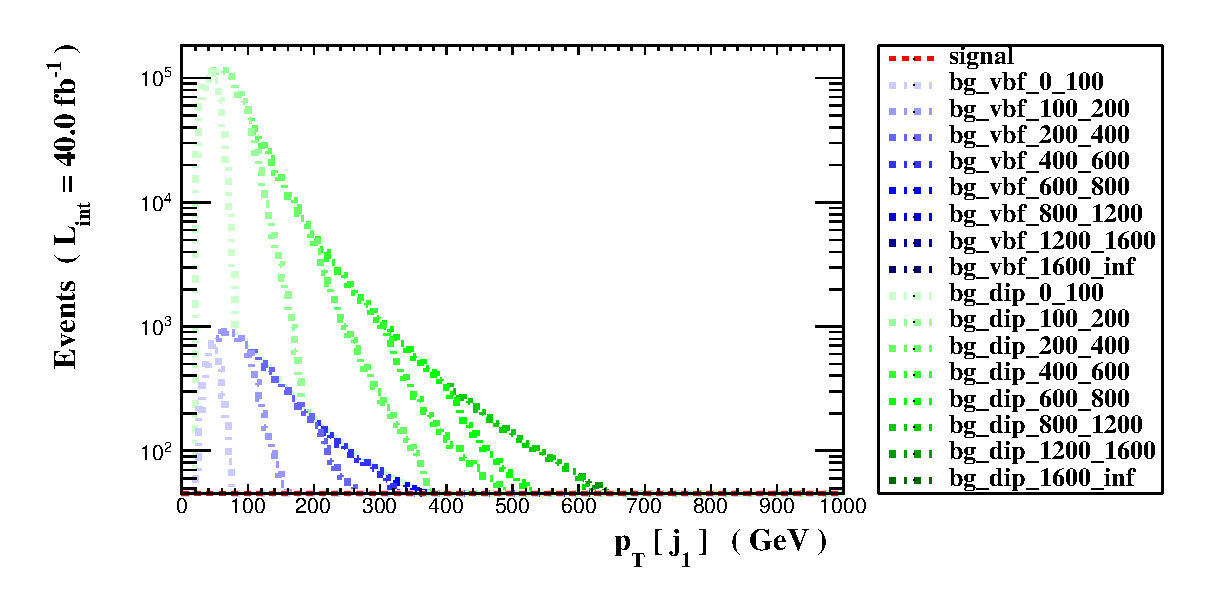
\includegraphics[scale=0.45]{selection_0.eps}\\
\caption{   }
  \end{center}
\end{figure}
      \newpage
\subsection{ Histogram 2}

\textbf{* Plot: ETA ( jets[1] ) }\\
   \begin{table}[H]
  \begin{center}
    \begin{tabular}{|m{23.0mm}|m{23.0mm}|m{18.0mm}|m{19.0mm}|m{19.0mm}|m{19.0mm}|m{19.0mm}|}
      \hline
      {\cellcolor{yellow}         Dataset}& {\cellcolor{yellow}         Integral}& {\cellcolor{yellow}         Entries per event}& {\cellcolor{yellow}         Mean}& {\cellcolor{yellow}         RMS}& {\cellcolor{yellow}         \% underflow}& {\cellcolor{yellow}         \% overflow}\\
      \hline
      {\cellcolor{white}         signal}& {\cellcolor{white}         4094}& {\cellcolor{white}         1.0}& {\cellcolor{white}         -0.0023996}& {\cellcolor{white}         1.616}& {\cellcolor{green}         0.0}& {\cellcolor{green}         0.0}\\
      \hline
      {\cellcolor{white}         bg\_vbf\_0\_100}& {\cellcolor{white}         3934}& {\cellcolor{white}         1.0}& {\cellcolor{white}         -0.00133609}& {\cellcolor{white}         2.635}& {\cellcolor{green}         0.0}& {\cellcolor{green}         0.0}\\
      \hline
      {\cellcolor{white}         bg\_vbf\_100\_200}& {\cellcolor{white}         8756}& {\cellcolor{white}         1.0}& {\cellcolor{white}         0.0043695}& {\cellcolor{white}         2.247}& {\cellcolor{green}         0.0}& {\cellcolor{green}         0.0}\\
      \hline
      {\cellcolor{white}         bg\_vbf\_200\_400}& {\cellcolor{white}         5358}& {\cellcolor{white}         1.0}& {\cellcolor{white}         0.00194377}& {\cellcolor{white}         1.965}& {\cellcolor{green}         0.0}& {\cellcolor{green}         0.0}\\
      \hline
      {\cellcolor{white}         bg\_vbf\_400\_600}& {\cellcolor{white}         983}& {\cellcolor{white}         1.0}& {\cellcolor{white}         -0.000999715}& {\cellcolor{white}         1.682}& {\cellcolor{green}         0.0}& {\cellcolor{green}         0.0}\\
      \hline
      {\cellcolor{white}         bg\_vbf\_600\_800}& {\cellcolor{white}         251}& {\cellcolor{white}         1.0}& {\cellcolor{white}         0.000513382}& {\cellcolor{white}         1.499}& {\cellcolor{green}         0.0}& {\cellcolor{green}         0.0}\\
      \hline
      {\cellcolor{white}         bg\_vbf\_800\_1200}& {\cellcolor{white}         114}& {\cellcolor{white}         1.0}& {\cellcolor{white}         -0.00310292}& {\cellcolor{white}         1.329}& {\cellcolor{green}         0.0}& {\cellcolor{green}         0.0}\\
      \hline
      {\cellcolor{white}         bg\_vbf\_1200\_1600}& {\cellcolor{white}         20.6}& {\cellcolor{white}         1.0}& {\cellcolor{white}         -0.000169046}& {\cellcolor{white}         1.134}& {\cellcolor{green}         0.0}& {\cellcolor{green}         0.0}\\
      \hline
      {\cellcolor{white}         bg\_vbf\_1600\_inf}& {\cellcolor{white}         7.66}& {\cellcolor{white}         1.0}& {\cellcolor{white}         0.00127081}& {\cellcolor{white}         0.9541}& {\cellcolor{green}         0.0}& {\cellcolor{green}         0.0}\\
      \hline
      {\cellcolor{white}         bg\_dip\_0\_100}& {\cellcolor{white}         714691}& {\cellcolor{white}         1.0}& {\cellcolor{white}         0.000508343}& {\cellcolor{white}         2.224}& {\cellcolor{green}         0.0}& {\cellcolor{green}         0.0}\\
      \hline
      {\cellcolor{white}         bg\_dip\_100\_200}& {\cellcolor{white}         855479}& {\cellcolor{white}         1.0}& {\cellcolor{white}         0.00260979}& {\cellcolor{white}         1.71}& {\cellcolor{green}         0.0}& {\cellcolor{green}         0.0}\\
      \hline
      {\cellcolor{white}         bg\_dip\_200\_400}& {\cellcolor{white}         234627}& {\cellcolor{white}         1.0}& {\cellcolor{white}         -0.0010006}& {\cellcolor{white}         1.468}& {\cellcolor{green}         0.0}& {\cellcolor{green}         0.0}\\
      \hline
      {\cellcolor{white}         bg\_dip\_400\_600}& {\cellcolor{white}         28616}& {\cellcolor{white}         1.0}& {\cellcolor{white}         -0.00170173}& {\cellcolor{white}         1.279}& {\cellcolor{green}         0.0}& {\cellcolor{green}         0.0}\\
      \hline
      {\cellcolor{white}         bg\_dip\_600\_800}& {\cellcolor{white}         6658}& {\cellcolor{white}         1.0}& {\cellcolor{white}         -0.0049065}& {\cellcolor{white}         1.157}& {\cellcolor{green}         0.0}& {\cellcolor{green}         0.0}\\
      \hline
      {\cellcolor{white}         bg\_dip\_800\_1200}& {\cellcolor{white}         2939}& {\cellcolor{white}         1.0}& {\cellcolor{white}         0.00133618}& {\cellcolor{white}         1.052}& {\cellcolor{green}         0.0}& {\cellcolor{green}         0.0}\\
      \hline
      {\cellcolor{white}         bg\_dip\_1200\_1600}& {\cellcolor{white}         513}& {\cellcolor{white}         1.0}& {\cellcolor{white}         -0.00486624}& {\cellcolor{white}         0.9226}& {\cellcolor{green}         0.0}& {\cellcolor{green}         0.0}\\
      \hline
      {\cellcolor{white}         bg\_dip\_1600\_inf}& {\cellcolor{white}         187}& {\cellcolor{white}         1.0}& {\cellcolor{white}         -0.00107396}& {\cellcolor{white}         0.8}& {\cellcolor{green}         0.0}& {\cellcolor{green}         0.0}\\
\hline
    \end{tabular}
  \end{center}
\end{table}

\begin{figure}[H]
  \begin{center}
    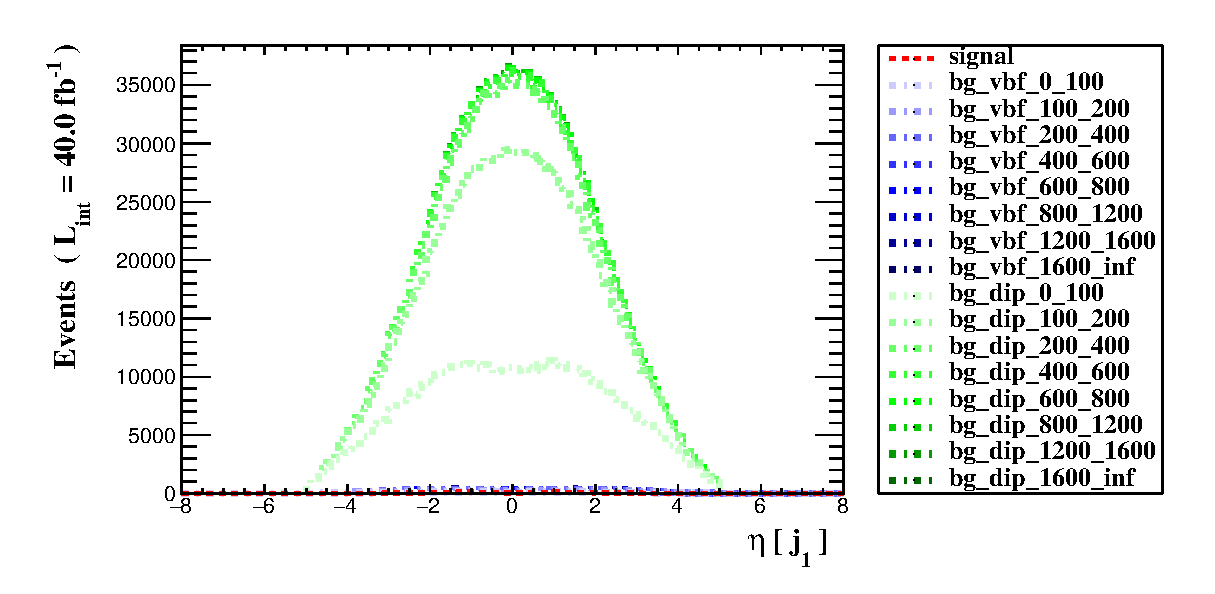
\includegraphics[scale=0.45]{selection_1.eps}\\
\caption{   }
  \end{center}
\end{figure}
      \newpage
\subsection{ Histogram 3}

\textbf{* Plot: PHI ( jets[1] ) }\\
   \begin{table}[H]
  \begin{center}
    \begin{tabular}{|m{23.0mm}|m{23.0mm}|m{18.0mm}|m{19.0mm}|m{19.0mm}|m{19.0mm}|m{19.0mm}|}
      \hline
      {\cellcolor{yellow}         Dataset}& {\cellcolor{yellow}         Integral}& {\cellcolor{yellow}         Entries per event}& {\cellcolor{yellow}         Mean}& {\cellcolor{yellow}         RMS}& {\cellcolor{yellow}         \% underflow}& {\cellcolor{yellow}         \% overflow}\\
      \hline
      {\cellcolor{white}         signal}& {\cellcolor{white}         4094}& {\cellcolor{white}         1.0}& {\cellcolor{white}         0.00102738}& {\cellcolor{white}         1.813}& {\cellcolor{green}         0.0}& {\cellcolor{green}         0.0}\\
      \hline
      {\cellcolor{white}         bg\_vbf\_0\_100}& {\cellcolor{white}         3934}& {\cellcolor{white}         1.0}& {\cellcolor{white}         0.00419195}& {\cellcolor{white}         1.813}& {\cellcolor{green}         0.0}& {\cellcolor{green}         0.0}\\
      \hline
      {\cellcolor{white}         bg\_vbf\_100\_200}& {\cellcolor{white}         8756}& {\cellcolor{white}         1.0}& {\cellcolor{white}         -0.00148977}& {\cellcolor{white}         1.814}& {\cellcolor{green}         0.0}& {\cellcolor{green}         0.0}\\
      \hline
      {\cellcolor{white}         bg\_vbf\_200\_400}& {\cellcolor{white}         5358}& {\cellcolor{white}         1.0}& {\cellcolor{white}         0.00192437}& {\cellcolor{white}         1.814}& {\cellcolor{green}         0.0}& {\cellcolor{green}         0.0}\\
      \hline
      {\cellcolor{white}         bg\_vbf\_400\_600}& {\cellcolor{white}         983}& {\cellcolor{white}         1.0}& {\cellcolor{white}         -0.00356173}& {\cellcolor{white}         1.813}& {\cellcolor{green}         0.0}& {\cellcolor{green}         0.0}\\
      \hline
      {\cellcolor{white}         bg\_vbf\_600\_800}& {\cellcolor{white}         251}& {\cellcolor{white}         1.0}& {\cellcolor{white}         -0.000882503}& {\cellcolor{white}         1.813}& {\cellcolor{green}         0.0}& {\cellcolor{green}         0.0}\\
      \hline
      {\cellcolor{white}         bg\_vbf\_800\_1200}& {\cellcolor{white}         114}& {\cellcolor{white}         1.0}& {\cellcolor{white}         -0.00348627}& {\cellcolor{white}         1.813}& {\cellcolor{green}         0.0}& {\cellcolor{green}         0.0}\\
      \hline
      {\cellcolor{white}         bg\_vbf\_1200\_1600}& {\cellcolor{white}         20.6}& {\cellcolor{white}         1.0}& {\cellcolor{white}         0.00205129}& {\cellcolor{white}         1.813}& {\cellcolor{green}         0.0}& {\cellcolor{green}         0.0}\\
      \hline
      {\cellcolor{white}         bg\_vbf\_1600\_inf}& {\cellcolor{white}         7.66}& {\cellcolor{white}         1.0}& {\cellcolor{white}         0.00218185}& {\cellcolor{white}         1.813}& {\cellcolor{green}         0.0}& {\cellcolor{green}         0.0}\\
      \hline
      {\cellcolor{white}         bg\_dip\_0\_100}& {\cellcolor{white}         714691}& {\cellcolor{white}         1.0}& {\cellcolor{white}         -0.00108067}& {\cellcolor{white}         1.816}& {\cellcolor{green}         0.0}& {\cellcolor{green}         0.0}\\
      \hline
      {\cellcolor{white}         bg\_dip\_100\_200}& {\cellcolor{white}         855479}& {\cellcolor{white}         1.0}& {\cellcolor{white}         0.00213448}& {\cellcolor{white}         1.814}& {\cellcolor{green}         0.0}& {\cellcolor{green}         0.0}\\
      \hline
      {\cellcolor{white}         bg\_dip\_200\_400}& {\cellcolor{white}         234627}& {\cellcolor{white}         1.0}& {\cellcolor{white}         -0.00158683}& {\cellcolor{white}         1.812}& {\cellcolor{green}         0.0}& {\cellcolor{green}         0.0}\\
      \hline
      {\cellcolor{white}         bg\_dip\_400\_600}& {\cellcolor{white}         28616}& {\cellcolor{white}         1.0}& {\cellcolor{white}         -0.00239958}& {\cellcolor{white}         1.813}& {\cellcolor{green}         0.0}& {\cellcolor{green}         0.0}\\
      \hline
      {\cellcolor{white}         bg\_dip\_600\_800}& {\cellcolor{white}         6658}& {\cellcolor{white}         1.0}& {\cellcolor{white}         0.00121432}& {\cellcolor{white}         1.814}& {\cellcolor{green}         0.0}& {\cellcolor{green}         0.0}\\
      \hline
      {\cellcolor{white}         bg\_dip\_800\_1200}& {\cellcolor{white}         2939}& {\cellcolor{white}         1.0}& {\cellcolor{white}         0.000396081}& {\cellcolor{white}         1.814}& {\cellcolor{green}         0.0}& {\cellcolor{green}         0.0}\\
      \hline
      {\cellcolor{white}         bg\_dip\_1200\_1600}& {\cellcolor{white}         513}& {\cellcolor{white}         1.0}& {\cellcolor{white}         6.26217e-05}& {\cellcolor{white}         1.814}& {\cellcolor{green}         0.0}& {\cellcolor{green}         0.0}\\
      \hline
      {\cellcolor{white}         bg\_dip\_1600\_inf}& {\cellcolor{white}         187}& {\cellcolor{white}         1.0}& {\cellcolor{white}         0.0014267}& {\cellcolor{white}         1.814}& {\cellcolor{green}         0.0}& {\cellcolor{green}         0.0}\\
\hline
    \end{tabular}
  \end{center}
\end{table}

\begin{figure}[H]
  \begin{center}
    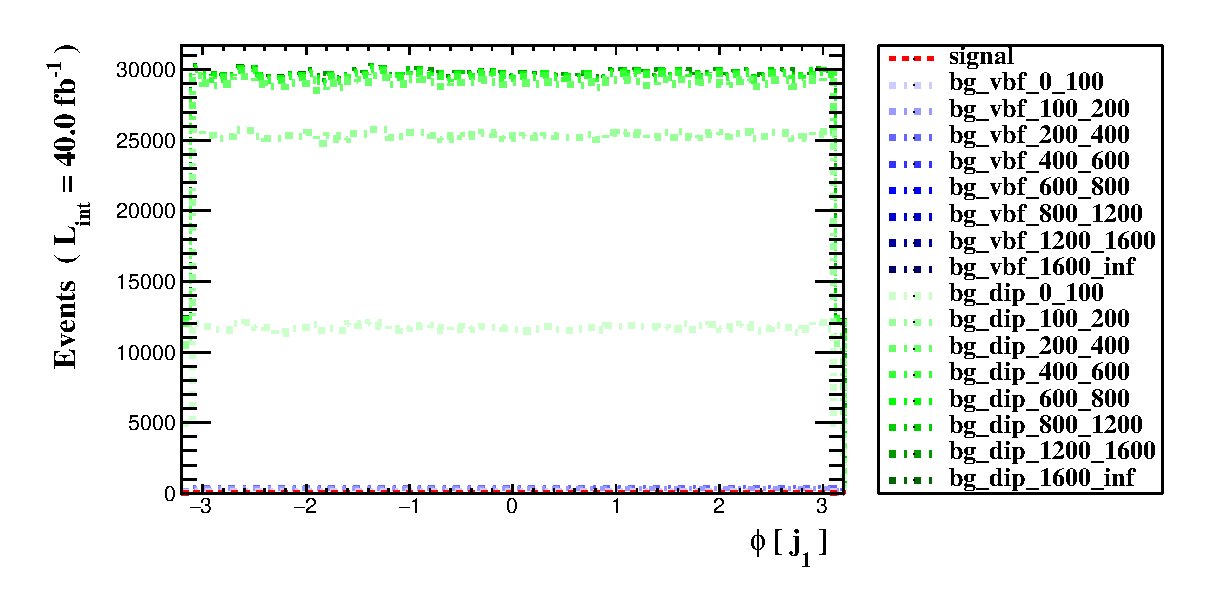
\includegraphics[scale=0.45]{selection_2.eps}\\
\caption{   }
  \end{center}
\end{figure}
      \newpage
\subsection{ Histogram 4}

\textbf{* Plot: PT ( jets[2] ) }\\
   \begin{table}[H]
  \begin{center}
    \begin{tabular}{|m{23.0mm}|m{23.0mm}|m{18.0mm}|m{19.0mm}|m{19.0mm}|m{19.0mm}|m{19.0mm}|}
      \hline
      {\cellcolor{yellow}         Dataset}& {\cellcolor{yellow}         Integral}& {\cellcolor{yellow}         Entries per event}& {\cellcolor{yellow}         Mean}& {\cellcolor{yellow}         RMS}& {\cellcolor{yellow}         \% underflow}& {\cellcolor{yellow}         \% overflow}\\
      \hline
      {\cellcolor{white}         signal}& {\cellcolor{white}         4094}& {\cellcolor{white}         1.0}& {\cellcolor{white}         161.87}& {\cellcolor{white}         136.0}& {\cellcolor{green}         0.0}& {\cellcolor{green}         3.02}\\
      \hline
      {\cellcolor{white}         bg\_vbf\_0\_100}& {\cellcolor{white}         3934}& {\cellcolor{white}         1.0}& {\cellcolor{white}         31.2504}& {\cellcolor{white}         7.217}& {\cellcolor{green}         0.0}& {\cellcolor{green}         0.0}\\
      \hline
      {\cellcolor{white}         bg\_vbf\_100\_200}& {\cellcolor{white}         8756}& {\cellcolor{white}         1.0}& {\cellcolor{white}         57.5348}& {\cellcolor{white}         16.74}& {\cellcolor{green}         0.0}& {\cellcolor{green}         0.0}\\
      \hline
      {\cellcolor{white}         bg\_vbf\_200\_400}& {\cellcolor{white}         5358}& {\cellcolor{white}         1.0}& {\cellcolor{white}         111.536}& {\cellcolor{white}         32.69}& {\cellcolor{green}         0.0}& {\cellcolor{green}         0.0}\\
      \hline
      {\cellcolor{white}         bg\_vbf\_400\_600}& {\cellcolor{white}         983}& {\cellcolor{white}         1.0}& {\cellcolor{white}         201.545}& {\cellcolor{white}         47.5}& {\cellcolor{green}         0.0}& {\cellcolor{green}         0.0}\\
      \hline
      {\cellcolor{white}         bg\_vbf\_600\_800}& {\cellcolor{white}         251}& {\cellcolor{white}         1.0}& {\cellcolor{white}         293.986}& {\cellcolor{white}         62.63}& {\cellcolor{green}         0.0}& {\cellcolor{green}         0.0}\\
      \hline
      {\cellcolor{white}         bg\_vbf\_800\_1200}& {\cellcolor{white}         114}& {\cellcolor{white}         1.0}& {\cellcolor{white}         415.077}& {\cellcolor{white}         90.48}& {\cellcolor{red}         0.0}& {\cellcolor{red}         15.1}\\
      \hline
      {\cellcolor{white}         bg\_vbf\_1200\_1600}& {\cellcolor{white}         20.6}& {\cellcolor{white}         1.0}& {\cellcolor{white}         613.849}& {\cellcolor{white}         108.4}& {\cellcolor{red}         0.0}& {\cellcolor{red}         90.47}\\
      \hline
      {\cellcolor{white}         bg\_vbf\_1600\_inf}& {\cellcolor{white}         7.66}& {\cellcolor{white}         1.0}& {\cellcolor{white}         917.972}& {\cellcolor{white}         221.8}& {\cellcolor{red}         0.0}& {\cellcolor{red}         98.03}\\
      \hline
      {\cellcolor{white}         bg\_dip\_0\_100}& {\cellcolor{white}         714691}& {\cellcolor{white}         1.0}& {\cellcolor{white}         29.8777}& {\cellcolor{white}         7.014}& {\cellcolor{green}         0.0}& {\cellcolor{green}         0.0}\\
      \hline
      {\cellcolor{white}         bg\_dip\_100\_200}& {\cellcolor{white}         855479}& {\cellcolor{white}         1.0}& {\cellcolor{white}         54.688}& {\cellcolor{white}         15.89}& {\cellcolor{green}         0.0}& {\cellcolor{green}         0.0}\\
      \hline
      {\cellcolor{white}         bg\_dip\_200\_400}& {\cellcolor{white}         234627}& {\cellcolor{white}         1.0}& {\cellcolor{white}         106.13}& {\cellcolor{white}         33.69}& {\cellcolor{green}         0.0}& {\cellcolor{green}         0.0}\\
      \hline
      {\cellcolor{white}         bg\_dip\_400\_600}& {\cellcolor{white}         28616}& {\cellcolor{white}         1.0}& {\cellcolor{white}         201.059}& {\cellcolor{white}         51.01}& {\cellcolor{green}         0.0}& {\cellcolor{green}         0.0}\\
      \hline
      {\cellcolor{white}         bg\_dip\_600\_800}& {\cellcolor{white}         6658}& {\cellcolor{white}         1.0}& {\cellcolor{white}         296.97}& {\cellcolor{white}         64.64}& {\cellcolor{green}         0.0}& {\cellcolor{green}         0.0}\\
      \hline
      {\cellcolor{white}         bg\_dip\_800\_1200}& {\cellcolor{white}         2939}& {\cellcolor{white}         1.0}& {\cellcolor{white}         421.627}& {\cellcolor{white}         88.69}& {\cellcolor{red}         0.0}& {\cellcolor{red}         16.13}\\
      \hline
      {\cellcolor{white}         bg\_dip\_1200\_1600}& {\cellcolor{white}         513}& {\cellcolor{white}         1.0}& {\cellcolor{white}         623.471}& {\cellcolor{white}         99.67}& {\cellcolor{red}         0.0}& {\cellcolor{red}         93.34}\\
      \hline
      {\cellcolor{white}         bg\_dip\_1600\_inf}& {\cellcolor{white}         187}& {\cellcolor{white}         1.0}& {\cellcolor{white}         926.302}& {\cellcolor{white}         210.5}& {\cellcolor{red}         0.0}& {\cellcolor{red}         98.92}\\
\hline
    \end{tabular}
  \end{center}
\end{table}

\begin{figure}[H]
  \begin{center}
    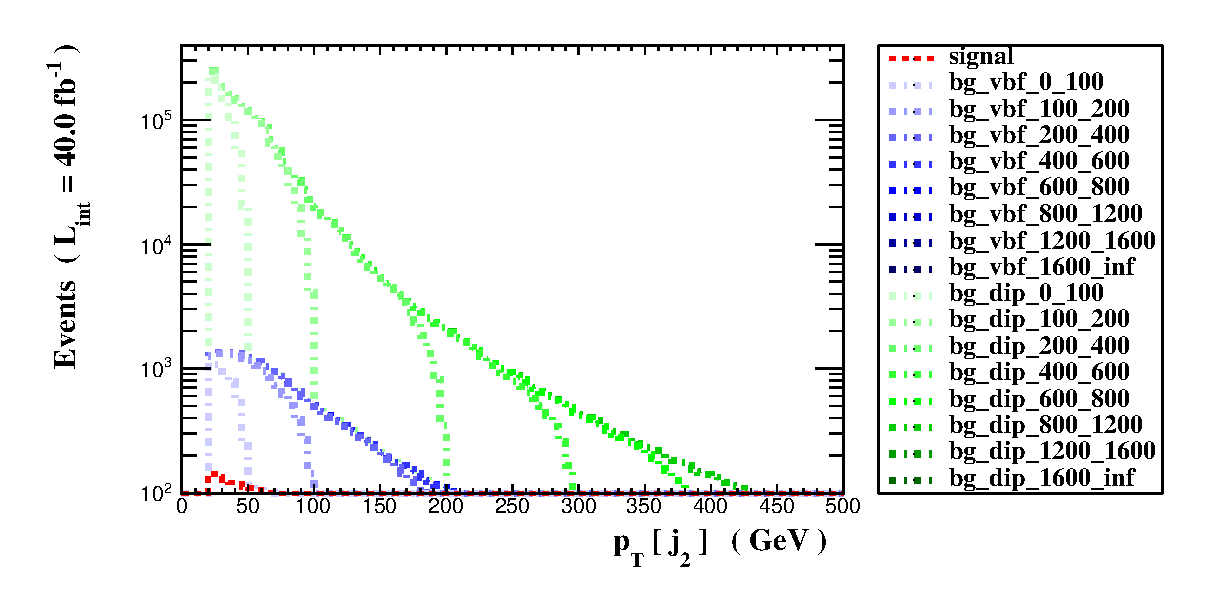
\includegraphics[scale=0.45]{selection_3.eps}\\
\caption{   }
  \end{center}
\end{figure}
      \newpage
\subsection{ Histogram 5}

\textbf{* Plot: ETA ( jets[2] ) }\\
   \begin{table}[H]
  \begin{center}
    \begin{tabular}{|m{23.0mm}|m{23.0mm}|m{18.0mm}|m{19.0mm}|m{19.0mm}|m{19.0mm}|m{19.0mm}|}
      \hline
      {\cellcolor{yellow}         Dataset}& {\cellcolor{yellow}         Integral}& {\cellcolor{yellow}         Entries per event}& {\cellcolor{yellow}         Mean}& {\cellcolor{yellow}         RMS}& {\cellcolor{yellow}         \% underflow}& {\cellcolor{yellow}         \% overflow}\\
      \hline
      {\cellcolor{white}         signal}& {\cellcolor{white}         4094}& {\cellcolor{white}         1.0}& {\cellcolor{white}         0.00500696}& {\cellcolor{white}         2.329}& {\cellcolor{green}         0.0}& {\cellcolor{green}         0.0}\\
      \hline
      {\cellcolor{white}         bg\_vbf\_0\_100}& {\cellcolor{white}         3934}& {\cellcolor{white}         1.0}& {\cellcolor{white}         -0.0019532}& {\cellcolor{white}         2.674}& {\cellcolor{green}         0.0}& {\cellcolor{green}         0.0}\\
      \hline
      {\cellcolor{white}         bg\_vbf\_100\_200}& {\cellcolor{white}         8756}& {\cellcolor{white}         1.0}& {\cellcolor{white}         -0.0066}& {\cellcolor{white}         2.371}& {\cellcolor{green}         0.0}& {\cellcolor{green}         0.0}\\
      \hline
      {\cellcolor{white}         bg\_vbf\_200\_400}& {\cellcolor{white}         5358}& {\cellcolor{white}         1.0}& {\cellcolor{white}         0.000228824}& {\cellcolor{white}         2.132}& {\cellcolor{green}         0.0}& {\cellcolor{green}         0.0}\\
      \hline
      {\cellcolor{white}         bg\_vbf\_400\_600}& {\cellcolor{white}         983}& {\cellcolor{white}         1.0}& {\cellcolor{white}         -0.000744275}& {\cellcolor{white}         1.863}& {\cellcolor{green}         0.0}& {\cellcolor{green}         0.0}\\
      \hline
      {\cellcolor{white}         bg\_vbf\_600\_800}& {\cellcolor{white}         251}& {\cellcolor{white}         1.0}& {\cellcolor{white}         -0.00168321}& {\cellcolor{white}         1.667}& {\cellcolor{green}         0.0}& {\cellcolor{green}         0.0}\\
      \hline
      {\cellcolor{white}         bg\_vbf\_800\_1200}& {\cellcolor{white}         114}& {\cellcolor{white}         1.0}& {\cellcolor{white}         -0.000452317}& {\cellcolor{white}         1.473}& {\cellcolor{green}         0.0}& {\cellcolor{green}         0.0}\\
      \hline
      {\cellcolor{white}         bg\_vbf\_1200\_1600}& {\cellcolor{white}         20.6}& {\cellcolor{white}         1.0}& {\cellcolor{white}         0.000595874}& {\cellcolor{white}         1.238}& {\cellcolor{green}         0.0}& {\cellcolor{green}         0.0}\\
      \hline
      {\cellcolor{white}         bg\_vbf\_1600\_inf}& {\cellcolor{white}         7.66}& {\cellcolor{white}         1.0}& {\cellcolor{white}         -0.00207042}& {\cellcolor{white}         1.017}& {\cellcolor{green}         0.0}& {\cellcolor{green}         0.0}\\
      \hline
      {\cellcolor{white}         bg\_dip\_0\_100}& {\cellcolor{white}         714691}& {\cellcolor{white}         1.0}& {\cellcolor{white}         1.01009e-05}& {\cellcolor{white}         2.147}& {\cellcolor{green}         0.0}& {\cellcolor{green}         0.0}\\
      \hline
      {\cellcolor{white}         bg\_dip\_100\_200}& {\cellcolor{white}         855479}& {\cellcolor{white}         1.0}& {\cellcolor{white}         -0.00108977}& {\cellcolor{white}         1.645}& {\cellcolor{green}         0.0}& {\cellcolor{green}         0.0}\\
      \hline
      {\cellcolor{white}         bg\_dip\_200\_400}& {\cellcolor{white}         234627}& {\cellcolor{white}         1.0}& {\cellcolor{white}         -0.00265008}& {\cellcolor{white}         1.446}& {\cellcolor{green}         0.0}& {\cellcolor{green}         0.0}\\
      \hline
      {\cellcolor{white}         bg\_dip\_400\_600}& {\cellcolor{white}         28616}& {\cellcolor{white}         1.0}& {\cellcolor{white}         -0.000387923}& {\cellcolor{white}         1.29}& {\cellcolor{green}         0.0}& {\cellcolor{green}         0.0}\\
      \hline
      {\cellcolor{white}         bg\_dip\_600\_800}& {\cellcolor{white}         6658}& {\cellcolor{white}         1.0}& {\cellcolor{white}         -0.000303381}& {\cellcolor{white}         1.182}& {\cellcolor{green}         0.0}& {\cellcolor{green}         0.0}\\
      \hline
      {\cellcolor{white}         bg\_dip\_800\_1200}& {\cellcolor{white}         2939}& {\cellcolor{white}         1.0}& {\cellcolor{white}         0.00119018}& {\cellcolor{white}         1.078}& {\cellcolor{green}         0.0}& {\cellcolor{green}         0.0}\\
      \hline
      {\cellcolor{white}         bg\_dip\_1200\_1600}& {\cellcolor{white}         513}& {\cellcolor{white}         1.0}& {\cellcolor{white}         -0.000424092}& {\cellcolor{white}         0.9457}& {\cellcolor{green}         0.0}& {\cellcolor{green}         0.0}\\
      \hline
      {\cellcolor{white}         bg\_dip\_1600\_inf}& {\cellcolor{white}         187}& {\cellcolor{white}         1.0}& {\cellcolor{white}         0.000907805}& {\cellcolor{white}         0.8179}& {\cellcolor{green}         0.0}& {\cellcolor{green}         0.0}\\
\hline
    \end{tabular}
  \end{center}
\end{table}

\begin{figure}[H]
  \begin{center}
    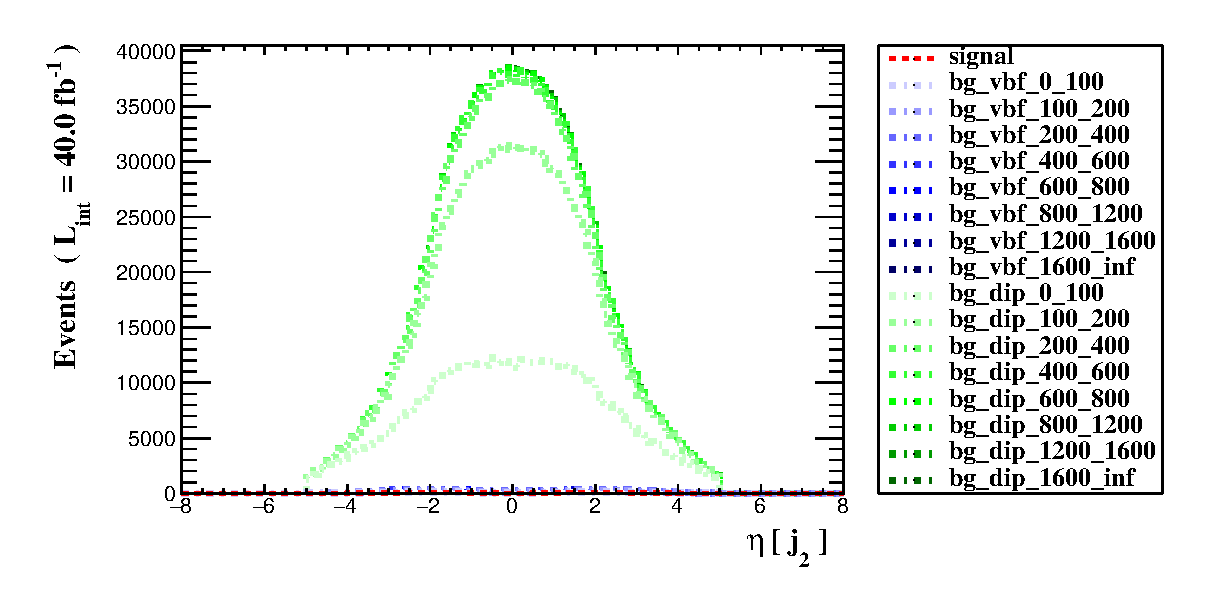
\includegraphics[scale=0.45]{selection_4.eps}\\
\caption{   }
  \end{center}
\end{figure}
      \newpage
\subsection{ Histogram 6}

\textbf{* Plot: PHI ( jets[2] ) }\\
   \begin{table}[H]
  \begin{center}
    \begin{tabular}{|m{23.0mm}|m{23.0mm}|m{18.0mm}|m{19.0mm}|m{19.0mm}|m{19.0mm}|m{19.0mm}|}
      \hline
      {\cellcolor{yellow}         Dataset}& {\cellcolor{yellow}         Integral}& {\cellcolor{yellow}         Entries per event}& {\cellcolor{yellow}         Mean}& {\cellcolor{yellow}         RMS}& {\cellcolor{yellow}         \% underflow}& {\cellcolor{yellow}         \% overflow}\\
      \hline
      {\cellcolor{white}         signal}& {\cellcolor{white}         4094}& {\cellcolor{white}         1.0}& {\cellcolor{white}         -0.00274458}& {\cellcolor{white}         1.814}& {\cellcolor{green}         0.0}& {\cellcolor{green}         0.0}\\
      \hline
      {\cellcolor{white}         bg\_vbf\_0\_100}& {\cellcolor{white}         3934}& {\cellcolor{white}         1.0}& {\cellcolor{white}         -0.00276363}& {\cellcolor{white}         1.814}& {\cellcolor{green}         0.0}& {\cellcolor{green}         0.0}\\
      \hline
      {\cellcolor{white}         bg\_vbf\_100\_200}& {\cellcolor{white}         8756}& {\cellcolor{white}         1.0}& {\cellcolor{white}         -3.00875e-05}& {\cellcolor{white}         1.815}& {\cellcolor{green}         0.0}& {\cellcolor{green}         0.0}\\
      \hline
      {\cellcolor{white}         bg\_vbf\_200\_400}& {\cellcolor{white}         5358}& {\cellcolor{white}         1.0}& {\cellcolor{white}         -0.00153572}& {\cellcolor{white}         1.814}& {\cellcolor{green}         0.0}& {\cellcolor{green}         0.0}\\
      \hline
      {\cellcolor{white}         bg\_vbf\_400\_600}& {\cellcolor{white}         983}& {\cellcolor{white}         1.0}& {\cellcolor{white}         0.00312538}& {\cellcolor{white}         1.814}& {\cellcolor{green}         0.0}& {\cellcolor{green}         0.0}\\
      \hline
      {\cellcolor{white}         bg\_vbf\_600\_800}& {\cellcolor{white}         251}& {\cellcolor{white}         1.0}& {\cellcolor{white}         0.00050346}& {\cellcolor{white}         1.815}& {\cellcolor{green}         0.0}& {\cellcolor{green}         0.0}\\
      \hline
      {\cellcolor{white}         bg\_vbf\_800\_1200}& {\cellcolor{white}         114}& {\cellcolor{white}         1.0}& {\cellcolor{white}         0.000132195}& {\cellcolor{white}         1.813}& {\cellcolor{green}         0.0}& {\cellcolor{green}         0.0}\\
      \hline
      {\cellcolor{white}         bg\_vbf\_1200\_1600}& {\cellcolor{white}         20.6}& {\cellcolor{white}         1.0}& {\cellcolor{white}         -0.0034209}& {\cellcolor{white}         1.815}& {\cellcolor{green}         0.0}& {\cellcolor{green}         0.0}\\
      \hline
      {\cellcolor{white}         bg\_vbf\_1600\_inf}& {\cellcolor{white}         7.66}& {\cellcolor{white}         1.0}& {\cellcolor{white}         -0.00282812}& {\cellcolor{white}         1.814}& {\cellcolor{green}         0.0}& {\cellcolor{green}         0.0}\\
      \hline
      {\cellcolor{white}         bg\_dip\_0\_100}& {\cellcolor{white}         714691}& {\cellcolor{white}         1.0}& {\cellcolor{white}         0.00324102}& {\cellcolor{white}         1.813}& {\cellcolor{green}         0.0}& {\cellcolor{green}         0.0}\\
      \hline
      {\cellcolor{white}         bg\_dip\_100\_200}& {\cellcolor{white}         855479}& {\cellcolor{white}         1.0}& {\cellcolor{white}         -0.00116298}& {\cellcolor{white}         1.815}& {\cellcolor{green}         0.0}& {\cellcolor{green}         0.0}\\
      \hline
      {\cellcolor{white}         bg\_dip\_200\_400}& {\cellcolor{white}         234627}& {\cellcolor{white}         1.0}& {\cellcolor{white}         0.000793162}& {\cellcolor{white}         1.815}& {\cellcolor{green}         0.0}& {\cellcolor{green}         0.0}\\
      \hline
      {\cellcolor{white}         bg\_dip\_400\_600}& {\cellcolor{white}         28616}& {\cellcolor{white}         1.0}& {\cellcolor{white}         -1.20627e-05}& {\cellcolor{white}         1.814}& {\cellcolor{green}         0.0}& {\cellcolor{green}         0.0}\\
      \hline
      {\cellcolor{white}         bg\_dip\_600\_800}& {\cellcolor{white}         6658}& {\cellcolor{white}         1.0}& {\cellcolor{white}         -0.00250468}& {\cellcolor{white}         1.815}& {\cellcolor{green}         0.0}& {\cellcolor{green}         0.0}\\
      \hline
      {\cellcolor{white}         bg\_dip\_800\_1200}& {\cellcolor{white}         2939}& {\cellcolor{white}         1.0}& {\cellcolor{white}         -0.000669513}& {\cellcolor{white}         1.813}& {\cellcolor{green}         0.0}& {\cellcolor{green}         0.0}\\
      \hline
      {\cellcolor{white}         bg\_dip\_1200\_1600}& {\cellcolor{white}         513}& {\cellcolor{white}         1.0}& {\cellcolor{white}         -0.00203746}& {\cellcolor{white}         1.813}& {\cellcolor{green}         0.0}& {\cellcolor{green}         0.0}\\
      \hline
      {\cellcolor{white}         bg\_dip\_1600\_inf}& {\cellcolor{white}         187}& {\cellcolor{white}         1.0}& {\cellcolor{white}         0.00234294}& {\cellcolor{white}         1.814}& {\cellcolor{green}         0.0}& {\cellcolor{green}         0.0}\\
\hline
    \end{tabular}
  \end{center}
\end{table}

\begin{figure}[H]
  \begin{center}
    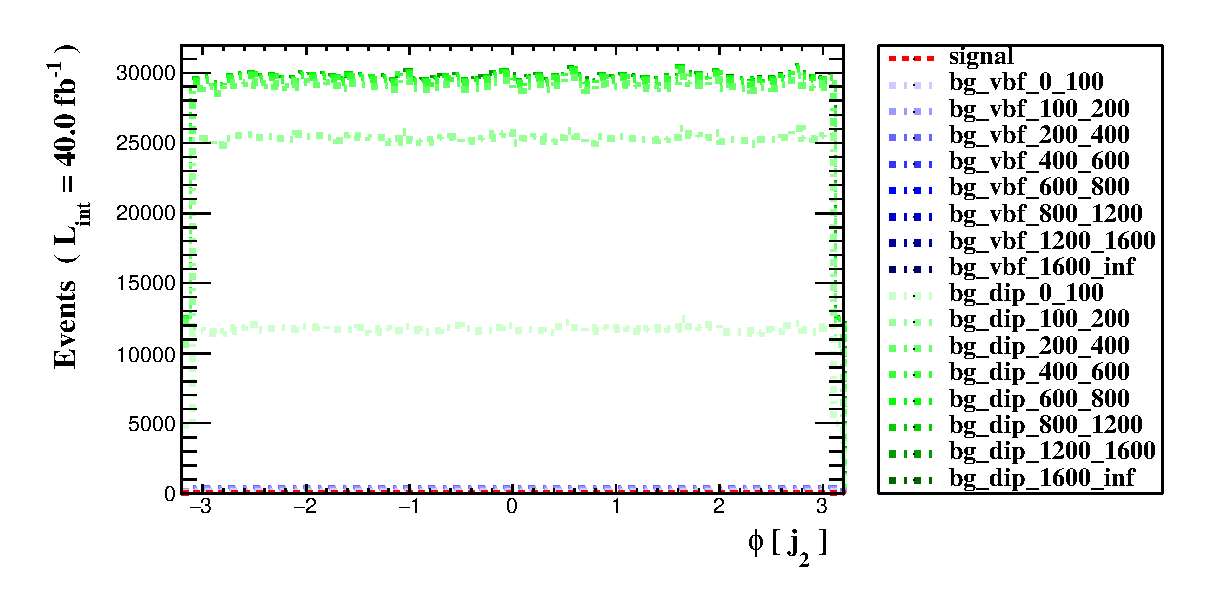
\includegraphics[scale=0.45]{selection_5.eps}\\
\caption{   }
  \end{center}
\end{figure}
      \newpage
\subsection{ Histogram 7}

\textbf{* Plot: DELTAR ( jets[1] , jets[2] ) }\\
   \begin{table}[H]
  \begin{center}
    \begin{tabular}{|m{23.0mm}|m{23.0mm}|m{18.0mm}|m{19.0mm}|m{19.0mm}|m{19.0mm}|m{19.0mm}|}
      \hline
      {\cellcolor{yellow}         Dataset}& {\cellcolor{yellow}         Integral}& {\cellcolor{yellow}         Entries per event}& {\cellcolor{yellow}         Mean}& {\cellcolor{yellow}         RMS}& {\cellcolor{yellow}         \% underflow}& {\cellcolor{yellow}         \% overflow}\\
      \hline
      {\cellcolor{white}         signal}& {\cellcolor{white}         4094}& {\cellcolor{white}         1.0}& {\cellcolor{white}         4.02835}& {\cellcolor{white}         1.056}& {\cellcolor{green}         0.0}& {\cellcolor{green}         0.0}\\
      \hline
      {\cellcolor{white}         bg\_vbf\_0\_100}& {\cellcolor{white}         3934}& {\cellcolor{white}         1.0}& {\cellcolor{white}         5.21509}& {\cellcolor{white}         1.267}& {\cellcolor{green}         0.0}& {\cellcolor{green}         0.0}\\
      \hline
      {\cellcolor{white}         bg\_vbf\_100\_200}& {\cellcolor{white}         8756}& {\cellcolor{white}         1.0}& {\cellcolor{white}         4.68485}& {\cellcolor{white}         1.264}& {\cellcolor{green}         0.0}& {\cellcolor{green}         0.0}\\
      \hline
      {\cellcolor{white}         bg\_vbf\_200\_400}& {\cellcolor{white}         5358}& {\cellcolor{white}         1.0}& {\cellcolor{white}         4.4049}& {\cellcolor{white}         1.096}& {\cellcolor{green}         0.0}& {\cellcolor{green}         0.0}\\
      \hline
      {\cellcolor{white}         bg\_vbf\_400\_600}& {\cellcolor{white}         983}& {\cellcolor{white}         1.0}& {\cellcolor{white}         4.11552}& {\cellcolor{white}         0.8948}& {\cellcolor{green}         0.0}& {\cellcolor{green}         0.0}\\
      \hline
      {\cellcolor{white}         bg\_vbf\_600\_800}& {\cellcolor{white}         251}& {\cellcolor{white}         1.0}& {\cellcolor{white}         3.92644}& {\cellcolor{white}         0.7722}& {\cellcolor{green}         0.0}& {\cellcolor{green}         0.0}\\
      \hline
      {\cellcolor{white}         bg\_vbf\_800\_1200}& {\cellcolor{white}         114}& {\cellcolor{white}         1.0}& {\cellcolor{white}         3.75826}& {\cellcolor{white}         0.6584}& {\cellcolor{green}         0.0}& {\cellcolor{green}         0.0}\\
      \hline
      {\cellcolor{white}         bg\_vbf\_1200\_1600}& {\cellcolor{white}         20.6}& {\cellcolor{white}         1.0}& {\cellcolor{white}         3.58482}& {\cellcolor{white}         0.5257}& {\cellcolor{green}         0.0}& {\cellcolor{green}         0.0}\\
      \hline
      {\cellcolor{white}         bg\_vbf\_1600\_inf}& {\cellcolor{white}         7.66}& {\cellcolor{white}         1.0}& {\cellcolor{white}         3.44779}& {\cellcolor{white}         0.4108}& {\cellcolor{green}         0.0}& {\cellcolor{green}         0.0}\\
      \hline
      {\cellcolor{white}         bg\_dip\_0\_100}& {\cellcolor{white}         714691}& {\cellcolor{white}         1.0}& {\cellcolor{white}         4.20916}& {\cellcolor{white}         0.7369}& {\cellcolor{green}         0.0}& {\cellcolor{green}         0.0}\\
      \hline
      {\cellcolor{white}         bg\_dip\_100\_200}& {\cellcolor{white}         855479}& {\cellcolor{white}         1.0}& {\cellcolor{white}         3.45656}& {\cellcolor{white}         0.6833}& {\cellcolor{green}         0.0}& {\cellcolor{green}         0.0}\\
      \hline
      {\cellcolor{white}         bg\_dip\_200\_400}& {\cellcolor{white}         234627}& {\cellcolor{white}         1.0}& {\cellcolor{white}         3.29993}& {\cellcolor{white}         0.6389}& {\cellcolor{green}         0.0}& {\cellcolor{green}         0.0}\\
      \hline
      {\cellcolor{white}         bg\_dip\_400\_600}& {\cellcolor{white}         28616}& {\cellcolor{white}         1.0}& {\cellcolor{white}         3.28686}& {\cellcolor{white}         0.5815}& {\cellcolor{green}         0.0}& {\cellcolor{green}         0.0}\\
      \hline
      {\cellcolor{white}         bg\_dip\_600\_800}& {\cellcolor{white}         6658}& {\cellcolor{white}         1.0}& {\cellcolor{white}         3.28486}& {\cellcolor{white}         0.5273}& {\cellcolor{green}         0.0}& {\cellcolor{green}         0.0}\\
      \hline
      {\cellcolor{white}         bg\_dip\_800\_1200}& {\cellcolor{white}         2939}& {\cellcolor{white}         1.0}& {\cellcolor{white}         3.28621}& {\cellcolor{white}         0.4662}& {\cellcolor{green}         0.0}& {\cellcolor{green}         0.0}\\
      \hline
      {\cellcolor{white}         bg\_dip\_1200\_1600}& {\cellcolor{white}         513}& {\cellcolor{white}         1.0}& {\cellcolor{white}         3.28098}& {\cellcolor{white}         0.3842}& {\cellcolor{green}         0.0}& {\cellcolor{green}         0.0}\\
      \hline
      {\cellcolor{white}         bg\_dip\_1600\_inf}& {\cellcolor{white}         187}& {\cellcolor{white}         1.0}& {\cellcolor{white}         3.26771}& {\cellcolor{white}         0.3022}& {\cellcolor{green}         0.0}& {\cellcolor{green}         0.0}\\
\hline
    \end{tabular}
  \end{center}
\end{table}

\begin{figure}[H]
  \begin{center}
    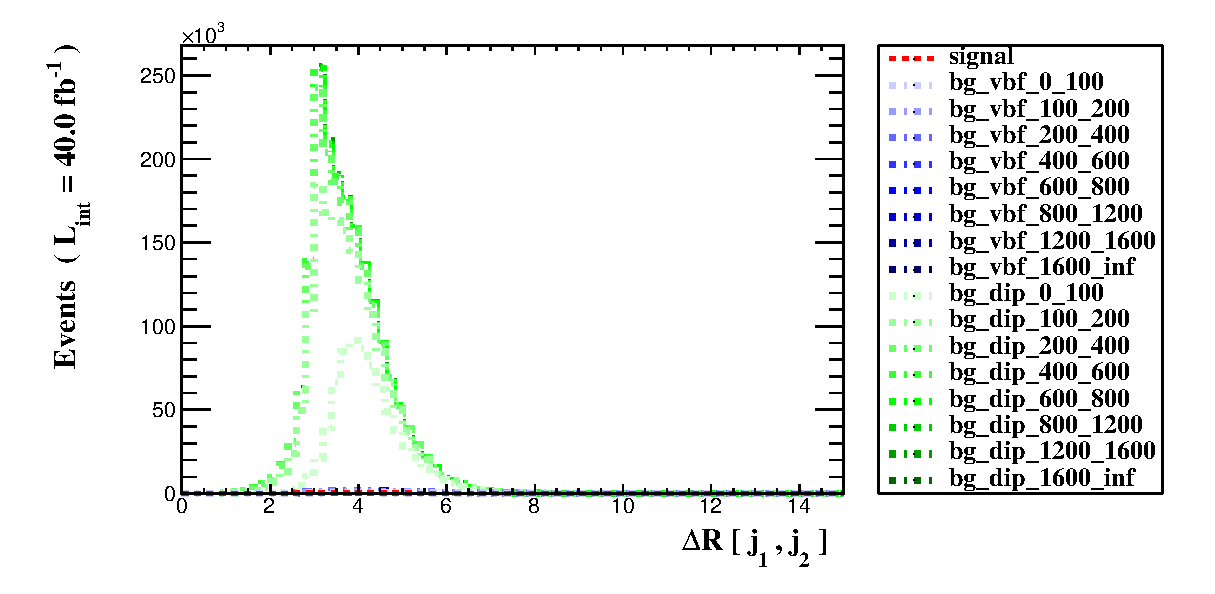
\includegraphics[scale=0.45]{selection_6.eps}\\
\caption{   }
  \end{center}
\end{figure}
      \newpage
\subsection{ Histogram 8}

\textbf{* Plot: M ( jets[1] jets[2] ) }\\
   \begin{table}[H]
  \begin{center}
    \begin{tabular}{|m{23.0mm}|m{23.0mm}|m{18.0mm}|m{19.0mm}|m{19.0mm}|m{19.0mm}|m{19.0mm}|}
      \hline
      {\cellcolor{yellow}         Dataset}& {\cellcolor{yellow}         Integral}& {\cellcolor{yellow}         Entries per event}& {\cellcolor{yellow}         Mean}& {\cellcolor{yellow}         RMS}& {\cellcolor{yellow}         \% underflow}& {\cellcolor{yellow}         \% overflow}\\
      \hline
      {\cellcolor{white}         signal}& {\cellcolor{white}         4094}& {\cellcolor{white}         1.0}& {\cellcolor{white}         1376.2}& {\cellcolor{white}         772.9}& {\cellcolor{green}         0.0}& {\cellcolor{green}         0.0}\\
      \hline
      {\cellcolor{white}         bg\_vbf\_0\_100}& {\cellcolor{white}         3934}& {\cellcolor{white}         1.0}& {\cellcolor{white}         469.964}& {\cellcolor{white}         412.4}& {\cellcolor{green}         0.0}& {\cellcolor{green}         0.0}\\
      \hline
      {\cellcolor{white}         bg\_vbf\_100\_200}& {\cellcolor{white}         8756}& {\cellcolor{white}         1.0}& {\cellcolor{white}         609.152}& {\cellcolor{white}         529.4}& {\cellcolor{green}         0.0}& {\cellcolor{green}         0.0}\\
      \hline
      {\cellcolor{white}         bg\_vbf\_200\_400}& {\cellcolor{white}         5358}& {\cellcolor{white}         1.0}& {\cellcolor{white}         888.626}& {\cellcolor{white}         671.3}& {\cellcolor{green}         0.0}& {\cellcolor{green}         0.0003082}\\
      \hline
      {\cellcolor{white}         bg\_vbf\_400\_600}& {\cellcolor{white}         983}& {\cellcolor{white}         1.0}& {\cellcolor{white}         1211.77}& {\cellcolor{white}         761.1}& {\cellcolor{green}         0.0}& {\cellcolor{green}         0.0006018}\\
      \hline
      {\cellcolor{white}         bg\_vbf\_600\_800}& {\cellcolor{white}         251}& {\cellcolor{white}         1.0}& {\cellcolor{white}         1465.23}& {\cellcolor{white}         805.1}& {\cellcolor{green}         0.0}& {\cellcolor{green}         0.001401}\\
      \hline
      {\cellcolor{white}         bg\_vbf\_800\_1200}& {\cellcolor{white}         114}& {\cellcolor{white}         1.0}& {\cellcolor{white}         1732.47}& {\cellcolor{white}         822.0}& {\cellcolor{green}         0.0}& {\cellcolor{green}         0.002495}\\
      \hline
      {\cellcolor{white}         bg\_vbf\_1200\_1600}& {\cellcolor{white}         20.6}& {\cellcolor{white}         1.0}& {\cellcolor{white}         2125.32}& {\cellcolor{white}         815.8}& {\cellcolor{green}         0.0}& {\cellcolor{green}         0.002832}\\
      \hline
      {\cellcolor{white}         bg\_vbf\_1600\_inf}& {\cellcolor{white}         7.66}& {\cellcolor{white}         1.0}& {\cellcolor{white}         2691.74}& {\cellcolor{white}         857.1}& {\cellcolor{green}         0.0}& {\cellcolor{green}         0.01037}\\
      \hline
      {\cellcolor{white}         bg\_dip\_0\_100}& {\cellcolor{white}         714691}& {\cellcolor{white}         1.0}& {\cellcolor{white}         202.321}& {\cellcolor{white}         105.0}& {\cellcolor{green}         0.0}& {\cellcolor{green}         0.0}\\
      \hline
      {\cellcolor{white}         bg\_dip\_100\_200}& {\cellcolor{white}         855479}& {\cellcolor{white}         1.0}& {\cellcolor{white}         222.194}& {\cellcolor{white}         129.4}& {\cellcolor{green}         0.0}& {\cellcolor{green}         0.0}\\
      \hline
      {\cellcolor{white}         bg\_dip\_200\_400}& {\cellcolor{white}         234627}& {\cellcolor{white}         1.0}& {\cellcolor{white}         364.432}& {\cellcolor{white}         195.6}& {\cellcolor{green}         0.0}& {\cellcolor{green}         0.0}\\
      \hline
      {\cellcolor{white}         bg\_dip\_400\_600}& {\cellcolor{white}         28616}& {\cellcolor{white}         1.0}& {\cellcolor{white}         626.063}& {\cellcolor{white}         277.8}& {\cellcolor{green}         0.0}& {\cellcolor{green}         0.0}\\
      \hline
      {\cellcolor{white}         bg\_dip\_600\_800}& {\cellcolor{white}         6658}& {\cellcolor{white}         1.0}& {\cellcolor{white}         872.986}& {\cellcolor{white}         337.8}& {\cellcolor{green}         0.0}& {\cellcolor{green}         0.0}\\
      \hline
      {\cellcolor{white}         bg\_dip\_800\_1200}& {\cellcolor{white}         2939}& {\cellcolor{white}         1.0}& {\cellcolor{white}         1178.48}& {\cellcolor{white}         408.8}& {\cellcolor{green}         0.0}& {\cellcolor{green}         0.0}\\
      \hline
      {\cellcolor{white}         bg\_dip\_1200\_1600}& {\cellcolor{white}         513}& {\cellcolor{white}         1.0}& {\cellcolor{white}         1647.88}& {\cellcolor{white}         468.4}& {\cellcolor{green}         0.0}& {\cellcolor{green}         0.0}\\
      \hline
      {\cellcolor{white}         bg\_dip\_1600\_inf}& {\cellcolor{white}         187}& {\cellcolor{white}         1.0}& {\cellcolor{white}         2311.56}& {\cellcolor{white}         635.4}& {\cellcolor{green}         0.0}& {\cellcolor{green}         0.0001923}\\
\hline
    \end{tabular}
  \end{center}
\end{table}

\begin{figure}[H]
  \begin{center}
    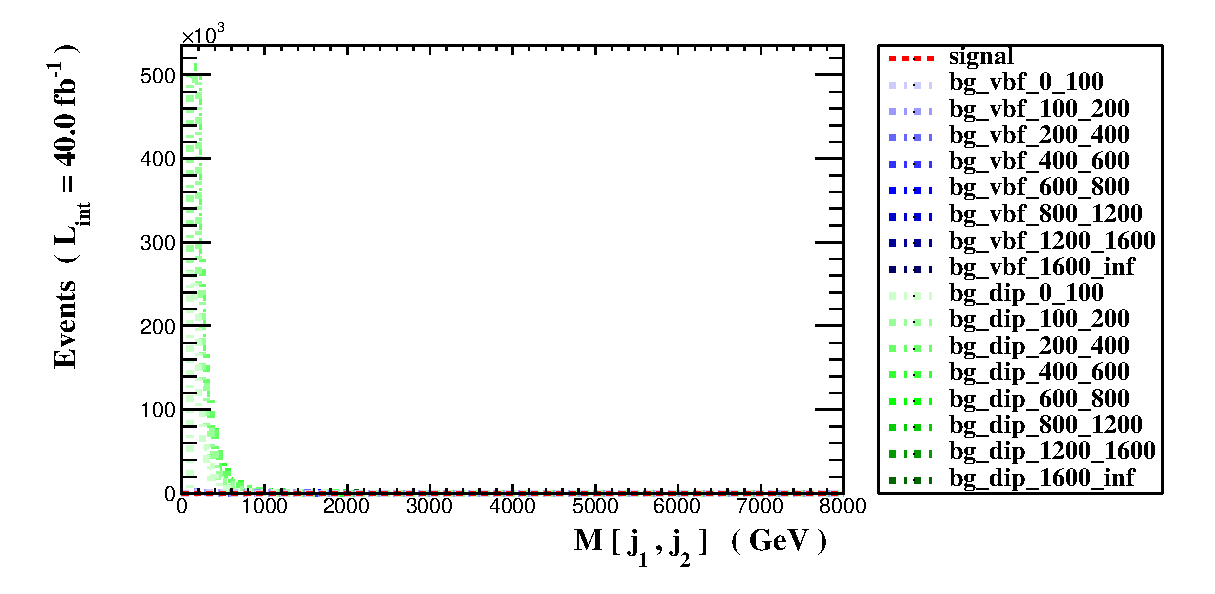
\includegraphics[scale=0.45]{selection_7.eps}\\
\caption{   }
  \end{center}
\end{figure}
      \newpage
\subsection{ Histogram 9}

\textbf{* Plot: MET}\\
   \begin{table}[H]
  \begin{center}
    \begin{tabular}{|m{23.0mm}|m{23.0mm}|m{18.0mm}|m{19.0mm}|m{19.0mm}|m{19.0mm}|m{19.0mm}|}
      \hline
      {\cellcolor{yellow}         Dataset}& {\cellcolor{yellow}         Integral}& {\cellcolor{yellow}         Entries per event}& {\cellcolor{yellow}         Mean}& {\cellcolor{yellow}         RMS}& {\cellcolor{yellow}         \% underflow}& {\cellcolor{yellow}         \% overflow}\\
      \hline
      {\cellcolor{white}         signal}& {\cellcolor{white}         4094}& {\cellcolor{white}         1.0}& {\cellcolor{white}         8.33083e-09}& {\cellcolor{white}         1.078e-08}& {\cellcolor{green}         0.0}& {\cellcolor{green}         0.0}\\
      \hline
      {\cellcolor{white}         bg\_vbf\_0\_100}& {\cellcolor{white}         3934}& {\cellcolor{white}         1.0}& {\cellcolor{white}         5.97855e-10}& {\cellcolor{white}         4.233e-10}& {\cellcolor{green}         0.0}& {\cellcolor{green}         0.0}\\
      \hline
      {\cellcolor{white}         bg\_vbf\_100\_200}& {\cellcolor{white}         8756}& {\cellcolor{white}         1.0}& {\cellcolor{white}         9.55638e-10}& {\cellcolor{white}         1.098e-09}& {\cellcolor{green}         0.0}& {\cellcolor{green}         0.0}\\
      \hline
      {\cellcolor{white}         bg\_vbf\_200\_400}& {\cellcolor{white}         5358}& {\cellcolor{white}         1.0}& {\cellcolor{white}         3.23057e-09}& {\cellcolor{white}         2.219e-09}& {\cellcolor{green}         0.0}& {\cellcolor{green}         0.0}\\
      \hline
      {\cellcolor{white}         bg\_vbf\_400\_600}& {\cellcolor{white}         983}& {\cellcolor{white}         1.0}& {\cellcolor{white}         4.52485e-09}& {\cellcolor{white}         2.611e-09}& {\cellcolor{green}         0.0}& {\cellcolor{green}         0.0}\\
      \hline
      {\cellcolor{white}         bg\_vbf\_600\_800}& {\cellcolor{white}         251}& {\cellcolor{white}         1.0}& {\cellcolor{white}         4.90226e-09}& {\cellcolor{white}         2.72e-09}& {\cellcolor{green}         0.0}& {\cellcolor{green}         0.0}\\
      \hline
      {\cellcolor{white}         bg\_vbf\_800\_1200}& {\cellcolor{white}         114}& {\cellcolor{white}         1.0}& {\cellcolor{white}         5.15622e-09}& {\cellcolor{white}         2.979e-09}& {\cellcolor{green}         0.0}& {\cellcolor{green}         0.0}\\
      \hline
      {\cellcolor{white}         bg\_vbf\_1200\_1600}& {\cellcolor{white}         20.6}& {\cellcolor{white}         1.0}& {\cellcolor{white}         5.81971e-09}& {\cellcolor{white}         5.339e-09}& {\cellcolor{green}         0.0}& {\cellcolor{green}         0.0}\\
      \hline
      {\cellcolor{white}         bg\_vbf\_1600\_inf}& {\cellcolor{white}         7.66}& {\cellcolor{white}         1.0}& {\cellcolor{white}         1.30635e-08}& {\cellcolor{white}         1.639e-08}& {\cellcolor{green}         0.0}& {\cellcolor{green}         0.0}\\
      \hline
      {\cellcolor{white}         bg\_dip\_0\_100}& {\cellcolor{white}         714691}& {\cellcolor{white}         1.0}& {\cellcolor{white}         5.87329e-10}& {\cellcolor{white}         4.134e-10}& {\cellcolor{green}         0.0}& {\cellcolor{green}         0.0}\\
      \hline
      {\cellcolor{white}         bg\_dip\_100\_200}& {\cellcolor{white}         855479}& {\cellcolor{white}         1.0}& {\cellcolor{white}         8.95295e-10}& {\cellcolor{white}         1.036e-09}& {\cellcolor{green}         0.0}& {\cellcolor{green}         0.0}\\
      \hline
      {\cellcolor{white}         bg\_dip\_200\_400}& {\cellcolor{white}         234627}& {\cellcolor{white}         1.0}& {\cellcolor{white}         3.11256e-09}& {\cellcolor{white}         2.186e-09}& {\cellcolor{green}         0.0}& {\cellcolor{green}         0.0}\\
      \hline
      {\cellcolor{white}         bg\_dip\_400\_600}& {\cellcolor{white}         28616}& {\cellcolor{white}         1.0}& {\cellcolor{white}         4.43451e-09}& {\cellcolor{white}         2.58e-09}& {\cellcolor{green}         0.0}& {\cellcolor{green}         0.0}\\
      \hline
      {\cellcolor{white}         bg\_dip\_600\_800}& {\cellcolor{white}         6658}& {\cellcolor{white}         1.0}& {\cellcolor{white}         4.80208e-09}& {\cellcolor{white}         2.678e-09}& {\cellcolor{green}         0.0}& {\cellcolor{green}         0.0}\\
      \hline
      {\cellcolor{white}         bg\_dip\_800\_1200}& {\cellcolor{white}         2939}& {\cellcolor{white}         1.0}& {\cellcolor{white}         5.06231e-09}& {\cellcolor{white}         3.026e-09}& {\cellcolor{green}         0.0}& {\cellcolor{green}         0.0}\\
      \hline
      {\cellcolor{white}         bg\_dip\_1200\_1600}& {\cellcolor{white}         513}& {\cellcolor{white}         1.0}& {\cellcolor{white}         5.58908e-09}& {\cellcolor{white}         4.823e-09}& {\cellcolor{green}         0.0}& {\cellcolor{green}         0.0}\\
      \hline
      {\cellcolor{white}         bg\_dip\_1600\_inf}& {\cellcolor{white}         187}& {\cellcolor{white}         1.0}& {\cellcolor{white}         1.25075e-08}& {\cellcolor{white}         1.605e-08}& {\cellcolor{green}         0.0}& {\cellcolor{green}         0.0}\\
\hline
    \end{tabular}
  \end{center}
\end{table}

\begin{figure}[H]
  \begin{center}
    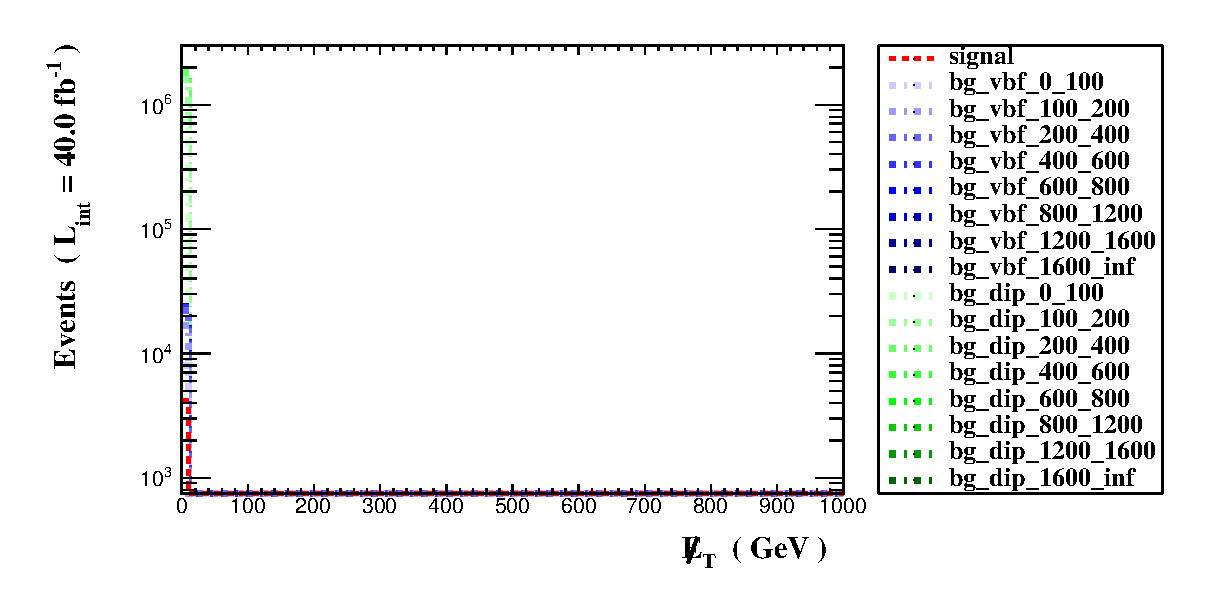
\includegraphics[scale=0.45]{selection_8.eps}\\
\caption{   }
  \end{center}
\end{figure}
      \newpage
\subsection{ Histogram 10}

\textbf{* Plot: sdETA ( jets[1] jets[2] ) }\\
   \begin{table}[H]
  \begin{center}
    \begin{tabular}{|m{23.0mm}|m{23.0mm}|m{18.0mm}|m{19.0mm}|m{19.0mm}|m{19.0mm}|m{19.0mm}|}
      \hline
      {\cellcolor{yellow}         Dataset}& {\cellcolor{yellow}         Integral}& {\cellcolor{yellow}         Entries per event}& {\cellcolor{yellow}         Mean}& {\cellcolor{yellow}         RMS}& {\cellcolor{yellow}         \% underflow}& {\cellcolor{yellow}         \% overflow}\\
      \hline
      {\cellcolor{white}         signal}& {\cellcolor{white}         4094}& {\cellcolor{white}         1.0}& {\cellcolor{white}         -0.00740656}& {\cellcolor{white}         3.704}& {\cellcolor{green}         0.2057}& {\cellcolor{green}         0.2022}\\
      \hline
      {\cellcolor{white}         bg\_vbf\_0\_100}& {\cellcolor{white}         3934}& {\cellcolor{white}         1.0}& {\cellcolor{white}         0.000617109}& {\cellcolor{white}         4.726}& {\cellcolor{green}         0.5803}& {\cellcolor{green}         0.6083}\\
      \hline
      {\cellcolor{white}         bg\_vbf\_100\_200}& {\cellcolor{white}         8756}& {\cellcolor{white}         1.0}& {\cellcolor{white}         0.0109695}& {\cellcolor{white}         4.015}& {\cellcolor{green}         0.1029}& {\cellcolor{green}         0.1176}\\
      \hline
      {\cellcolor{white}         bg\_vbf\_200\_400}& {\cellcolor{white}         5358}& {\cellcolor{white}         1.0}& {\cellcolor{white}         0.00171495}& {\cellcolor{white}         3.569}& {\cellcolor{green}         0.004928}& {\cellcolor{green}         0.003696}\\
      \hline
      {\cellcolor{white}         bg\_vbf\_400\_600}& {\cellcolor{white}         983}& {\cellcolor{white}         1.0}& {\cellcolor{white}         -0.000255441}& {\cellcolor{white}         3.09}& {\cellcolor{green}         0.0}& {\cellcolor{green}         0.0}\\
      \hline
      {\cellcolor{white}         bg\_vbf\_600\_800}& {\cellcolor{white}         251}& {\cellcolor{white}         1.0}& {\cellcolor{white}         0.00219659}& {\cellcolor{white}         2.754}& {\cellcolor{green}         0.0}& {\cellcolor{green}         0.0}\\
      \hline
      {\cellcolor{white}         bg\_vbf\_800\_1200}& {\cellcolor{white}         114}& {\cellcolor{white}         1.0}& {\cellcolor{white}         -0.0026506}& {\cellcolor{white}         2.428}& {\cellcolor{green}         0.0}& {\cellcolor{green}         0.0}\\
      \hline
      {\cellcolor{white}         bg\_vbf\_1200\_1600}& {\cellcolor{white}         20.6}& {\cellcolor{white}         1.0}& {\cellcolor{white}         -0.00076492}& {\cellcolor{white}         2.046}& {\cellcolor{green}         0.0}& {\cellcolor{green}         0.0}\\
      \hline
      {\cellcolor{white}         bg\_vbf\_1600\_inf}& {\cellcolor{white}         7.66}& {\cellcolor{white}         1.0}& {\cellcolor{white}         0.00334122}& {\cellcolor{white}         1.694}& {\cellcolor{green}         0.0}& {\cellcolor{green}         0.0}\\
      \hline
      {\cellcolor{white}         bg\_dip\_0\_100}& {\cellcolor{white}         714691}& {\cellcolor{white}         1.0}& {\cellcolor{white}         0.000498242}& {\cellcolor{white}         3.363}& {\cellcolor{green}         0.0}& {\cellcolor{green}         0.0007299}\\
      \hline
      {\cellcolor{white}         bg\_dip\_100\_200}& {\cellcolor{white}         855479}& {\cellcolor{white}         1.0}& {\cellcolor{white}         0.00369956}& {\cellcolor{white}         2.156}& {\cellcolor{green}         0.0001229}& {\cellcolor{green}         0.0}\\
      \hline
      {\cellcolor{white}         bg\_dip\_200\_400}& {\cellcolor{white}         234627}& {\cellcolor{white}         1.0}& {\cellcolor{white}         0.00164949}& {\cellcolor{white}         1.795}& {\cellcolor{green}         0.0}& {\cellcolor{green}         0.0}\\
      \hline
      {\cellcolor{white}         bg\_dip\_400\_600}& {\cellcolor{white}         28616}& {\cellcolor{white}         1.0}& {\cellcolor{white}         -0.00131381}& {\cellcolor{white}         1.639}& {\cellcolor{green}         0.0}& {\cellcolor{green}         0.0}\\
      \hline
      {\cellcolor{white}         bg\_dip\_600\_800}& {\cellcolor{white}         6658}& {\cellcolor{white}         1.0}& {\cellcolor{white}         -0.00460312}& {\cellcolor{white}         1.539}& {\cellcolor{green}         0.0}& {\cellcolor{green}         0.0}\\
      \hline
      {\cellcolor{white}         bg\_dip\_800\_1200}& {\cellcolor{white}         2939}& {\cellcolor{white}         1.0}& {\cellcolor{white}         0.000145998}& {\cellcolor{white}         1.448}& {\cellcolor{green}         0.0}& {\cellcolor{green}         0.0}\\
      \hline
      {\cellcolor{white}         bg\_dip\_1200\_1600}& {\cellcolor{white}         513}& {\cellcolor{white}         1.0}& {\cellcolor{white}         -0.00444215}& {\cellcolor{white}         1.327}& {\cellcolor{green}         0.0}& {\cellcolor{green}         0.0}\\
      \hline
      {\cellcolor{white}         bg\_dip\_1600\_inf}& {\cellcolor{white}         187}& {\cellcolor{white}         1.0}& {\cellcolor{white}         -0.00198176}& {\cellcolor{white}         1.196}& {\cellcolor{green}         0.0}& {\cellcolor{green}         0.0}\\
\hline
    \end{tabular}
  \end{center}
\end{table}

\begin{figure}[H]
  \begin{center}
    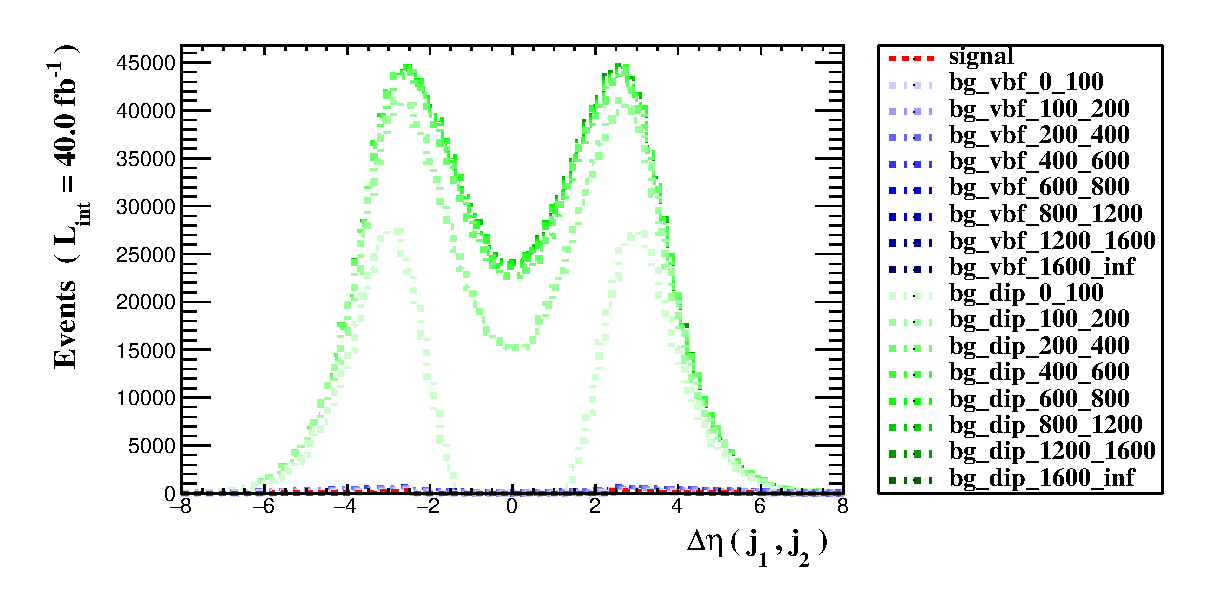
\includegraphics[scale=0.45]{selection_9.eps}\\
\caption{   }
  \end{center}
\end{figure}
      \newpage
\subsection{ Histogram 11}

\textbf{* Plot: M ( a[1] a[2] ) }\\
   \begin{table}[H]
  \begin{center}
    \begin{tabular}{|m{23.0mm}|m{23.0mm}|m{18.0mm}|m{19.0mm}|m{19.0mm}|m{19.0mm}|m{19.0mm}|}
      \hline
      {\cellcolor{yellow}         Dataset}& {\cellcolor{yellow}         Integral}& {\cellcolor{yellow}         Entries per event}& {\cellcolor{yellow}         Mean}& {\cellcolor{yellow}         RMS}& {\cellcolor{yellow}         \% underflow}& {\cellcolor{yellow}         \% overflow}\\
      \hline
      {\cellcolor{white}         signal}& {\cellcolor{white}         4094}& {\cellcolor{white}         1.0}& {\cellcolor{white}         950.206}& {\cellcolor{white}         725.5}& {\cellcolor{red}         0.0}& {\cellcolor{red}         36.84}\\
      \hline
      {\cellcolor{white}         bg\_vbf\_0\_100}& {\cellcolor{white}         3934}& {\cellcolor{white}         1.0}& {\cellcolor{white}         59.2471}& {\cellcolor{white}         49.28}& {\cellcolor{green}         0.0}& {\cellcolor{green}         0.002778}\\
      \hline
      {\cellcolor{white}         bg\_vbf\_100\_200}& {\cellcolor{white}         8756}& {\cellcolor{white}         1.0}& {\cellcolor{white}         70.2822}& {\cellcolor{white}         64.56}& {\cellcolor{green}         0.0}& {\cellcolor{green}         0.01548}\\
      \hline
      {\cellcolor{white}         bg\_vbf\_200\_400}& {\cellcolor{white}         5358}& {\cellcolor{white}         1.0}& {\cellcolor{white}         92.2723}& {\cellcolor{white}         92.82}& {\cellcolor{green}         0.0}& {\cellcolor{green}         0.0622}\\
      \hline
      {\cellcolor{white}         bg\_vbf\_400\_600}& {\cellcolor{white}         983}& {\cellcolor{white}         1.0}& {\cellcolor{white}         117.071}& {\cellcolor{white}         124.4}& {\cellcolor{green}         0.0}& {\cellcolor{green}         0.1777}\\
      \hline
      {\cellcolor{white}         bg\_vbf\_600\_800}& {\cellcolor{white}         251}& {\cellcolor{white}         1.0}& {\cellcolor{white}         132.524}& {\cellcolor{white}         146.0}& {\cellcolor{green}         0.0}& {\cellcolor{green}         0.3347}\\
      \hline
      {\cellcolor{white}         bg\_vbf\_800\_1200}& {\cellcolor{white}         114}& {\cellcolor{white}         1.0}& {\cellcolor{white}         143.801}& {\cellcolor{white}         162.6}& {\cellcolor{green}         0.0}& {\cellcolor{green}         0.5078}\\
      \hline
      {\cellcolor{white}         bg\_vbf\_1200\_1600}& {\cellcolor{white}         20.6}& {\cellcolor{white}         1.0}& {\cellcolor{white}         153.519}& {\cellcolor{white}         177.9}& {\cellcolor{green}         0.0}& {\cellcolor{green}         0.6926}\\
      \hline
      {\cellcolor{white}         bg\_vbf\_1600\_inf}& {\cellcolor{white}         7.66}& {\cellcolor{white}         1.0}& {\cellcolor{white}         159.525}& {\cellcolor{white}         184.7}& {\cellcolor{green}         0.0}& {\cellcolor{green}         0.7897}\\
      \hline
      {\cellcolor{white}         bg\_dip\_0\_100}& {\cellcolor{white}         714691}& {\cellcolor{white}         1.0}& {\cellcolor{white}         48.4767}& {\cellcolor{white}         39.08}& {\cellcolor{green}         0.0}& {\cellcolor{green}         0.002553}\\
      \hline
      {\cellcolor{white}         bg\_dip\_100\_200}& {\cellcolor{white}         855479}& {\cellcolor{white}         1.0}& {\cellcolor{white}         55.4245}& {\cellcolor{white}         50.97}& {\cellcolor{green}         0.0}& {\cellcolor{green}         0.004558}\\
      \hline
      {\cellcolor{white}         bg\_dip\_200\_400}& {\cellcolor{white}         234627}& {\cellcolor{white}         1.0}& {\cellcolor{white}         74.3979}& {\cellcolor{white}         76.83}& {\cellcolor{green}         0.0}& {\cellcolor{green}         0.0267}\\
      \hline
      {\cellcolor{white}         bg\_dip\_400\_600}& {\cellcolor{white}         28616}& {\cellcolor{white}         1.0}& {\cellcolor{white}         95.1626}& {\cellcolor{white}         107.9}& {\cellcolor{green}         0.0}& {\cellcolor{green}         0.1108}\\
      \hline
      {\cellcolor{white}         bg\_dip\_600\_800}& {\cellcolor{white}         6658}& {\cellcolor{white}         1.0}& {\cellcolor{white}         108.836}& {\cellcolor{white}         127.8}& {\cellcolor{green}         0.0}& {\cellcolor{green}         0.2203}\\
      \hline
      {\cellcolor{white}         bg\_dip\_800\_1200}& {\cellcolor{white}         2939}& {\cellcolor{white}         1.0}& {\cellcolor{white}         119.749}& {\cellcolor{white}         143.7}& {\cellcolor{green}         0.0}& {\cellcolor{green}         0.3484}\\
      \hline
      {\cellcolor{white}         bg\_dip\_1200\_1600}& {\cellcolor{white}         513}& {\cellcolor{white}         1.0}& {\cellcolor{white}         131.534}& {\cellcolor{white}         157.2}& {\cellcolor{green}         0.0}& {\cellcolor{green}         0.4736}\\
      \hline
      {\cellcolor{white}         bg\_dip\_1600\_inf}& {\cellcolor{white}         187}& {\cellcolor{white}         1.0}& {\cellcolor{white}         143.672}& {\cellcolor{white}         167.2}& {\cellcolor{green}         0.0}& {\cellcolor{green}         0.5656}\\
\hline
    \end{tabular}
  \end{center}
\end{table}

\begin{figure}[H]
  \begin{center}
    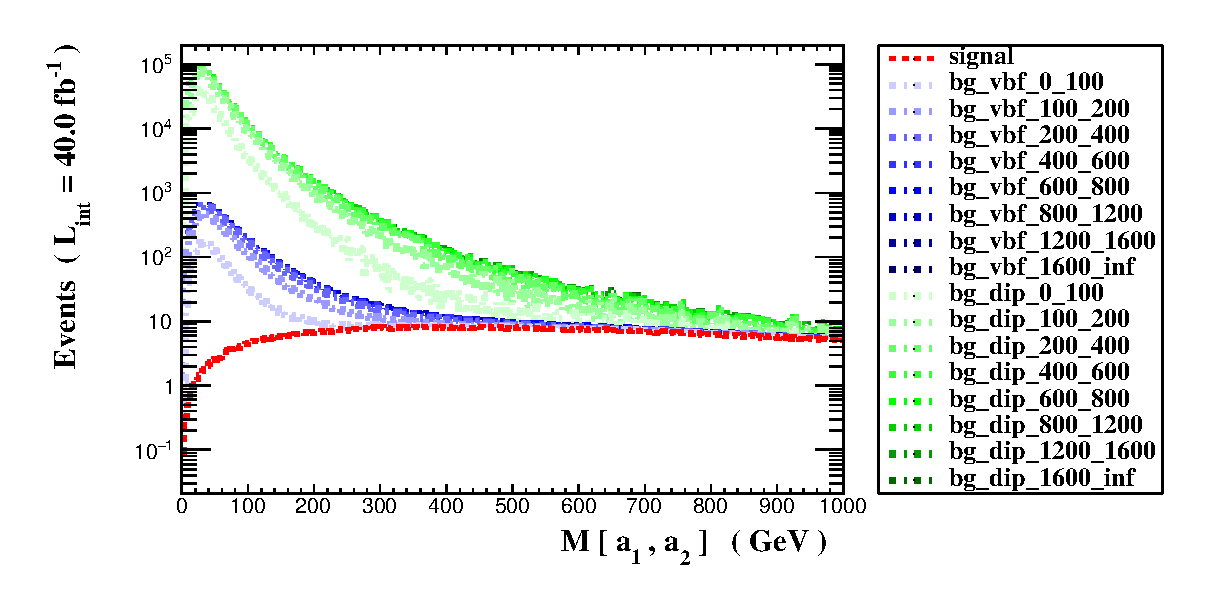
\includegraphics[scale=0.45]{selection_10.eps}\\
\caption{   }
  \end{center}
\end{figure}
      \newpage
\subsection{ Histogram 12}

\textbf{* Plot: PT ( a[1] ) }\\
   \begin{table}[H]
  \begin{center}
    \begin{tabular}{|m{23.0mm}|m{23.0mm}|m{18.0mm}|m{19.0mm}|m{19.0mm}|m{19.0mm}|m{19.0mm}|}
      \hline
      {\cellcolor{yellow}         Dataset}& {\cellcolor{yellow}         Integral}& {\cellcolor{yellow}         Entries per event}& {\cellcolor{yellow}         Mean}& {\cellcolor{yellow}         RMS}& {\cellcolor{yellow}         \% underflow}& {\cellcolor{yellow}         \% overflow}\\
      \hline
      {\cellcolor{white}         signal}& {\cellcolor{white}         4094}& {\cellcolor{white}         1.0}& {\cellcolor{white}         588.092}& {\cellcolor{white}         368.7}& {\cellcolor{orange}         0.0}& {\cellcolor{orange}         12.98}\\
      \hline
      {\cellcolor{white}         bg\_vbf\_0\_100}& {\cellcolor{white}         3934}& {\cellcolor{white}         1.0}& {\cellcolor{white}         33.0393}& {\cellcolor{white}         18.87}& {\cellcolor{green}         0.0}& {\cellcolor{green}         0.0}\\
      \hline
      {\cellcolor{white}         bg\_vbf\_100\_200}& {\cellcolor{white}         8756}& {\cellcolor{white}         1.0}& {\cellcolor{white}         46.4939}& {\cellcolor{white}         31.54}& {\cellcolor{green}         0.0}& {\cellcolor{green}         0.0}\\
      \hline
      {\cellcolor{white}         bg\_vbf\_200\_400}& {\cellcolor{white}         5358}& {\cellcolor{white}         1.0}& {\cellcolor{white}         72.005}& {\cellcolor{white}         60.42}& {\cellcolor{green}         0.0}& {\cellcolor{green}         0.000308}\\
      \hline
      {\cellcolor{white}         bg\_vbf\_400\_600}& {\cellcolor{white}         983}& {\cellcolor{white}         1.0}& {\cellcolor{white}         106.886}& {\cellcolor{white}         103.6}& {\cellcolor{green}         0.0}& {\cellcolor{green}         0.002407}\\
      \hline
      {\cellcolor{white}         bg\_vbf\_600\_800}& {\cellcolor{white}         251}& {\cellcolor{white}         1.0}& {\cellcolor{white}         132.381}& {\cellcolor{white}         141.7}& {\cellcolor{green}         0.0}& {\cellcolor{green}         0.009208}\\
      \hline
      {\cellcolor{white}         bg\_vbf\_800\_1200}& {\cellcolor{white}         114}& {\cellcolor{white}         1.0}& {\cellcolor{white}         154.148}& {\cellcolor{white}         182.0}& {\cellcolor{green}         0.0}& {\cellcolor{green}         0.3163}\\
      \hline
      {\cellcolor{white}         bg\_vbf\_1200\_1600}& {\cellcolor{white}         20.6}& {\cellcolor{white}         1.0}& {\cellcolor{white}         172.887}& {\cellcolor{white}         223.7}& {\cellcolor{green}         0.0}& {\cellcolor{green}         1.906}\\
      \hline
      {\cellcolor{white}         bg\_vbf\_1600\_inf}& {\cellcolor{white}         7.66}& {\cellcolor{white}         1.0}& {\cellcolor{white}         181.168}& {\cellcolor{white}         246.2}& {\cellcolor{green}         0.0}& {\cellcolor{green}         2.06}\\
      \hline
      {\cellcolor{white}         bg\_dip\_0\_100}& {\cellcolor{white}         714691}& {\cellcolor{white}         1.0}& {\cellcolor{white}         29.8019}& {\cellcolor{white}         18.74}& {\cellcolor{green}         0.0}& {\cellcolor{green}         0.0}\\
      \hline
      {\cellcolor{white}         bg\_dip\_100\_200}& {\cellcolor{white}         855479}& {\cellcolor{white}         1.0}& {\cellcolor{white}         42.2098}& {\cellcolor{white}         31.98}& {\cellcolor{green}         0.0}& {\cellcolor{green}         0.0001231}\\
      \hline
      {\cellcolor{white}         bg\_dip\_200\_400}& {\cellcolor{white}         234627}& {\cellcolor{white}         1.0}& {\cellcolor{white}         67.1266}& {\cellcolor{white}         63.03}& {\cellcolor{green}         0.0}& {\cellcolor{green}         9.834e-05}\\
      \hline
      {\cellcolor{white}         bg\_dip\_400\_600}& {\cellcolor{white}         28616}& {\cellcolor{white}         1.0}& {\cellcolor{white}         95.4197}& {\cellcolor{white}         106.8}& {\cellcolor{green}         0.0}& {\cellcolor{green}         0.001258}\\
      \hline
      {\cellcolor{white}         bg\_dip\_600\_800}& {\cellcolor{white}         6658}& {\cellcolor{white}         1.0}& {\cellcolor{white}         113.382}& {\cellcolor{white}         139.4}& {\cellcolor{green}         0.0}& {\cellcolor{green}         0.00999}\\
      \hline
      {\cellcolor{white}         bg\_dip\_800\_1200}& {\cellcolor{white}         2939}& {\cellcolor{white}         1.0}& {\cellcolor{white}         126.721}& {\cellcolor{white}         168.3}& {\cellcolor{green}         0.0}& {\cellcolor{green}         0.3807}\\
      \hline
      {\cellcolor{white}         bg\_dip\_1200\_1600}& {\cellcolor{white}         513}& {\cellcolor{white}         1.0}& {\cellcolor{white}         138.701}& {\cellcolor{white}         193.4}& {\cellcolor{green}         0.0}& {\cellcolor{green}         1.426}\\
      \hline
      {\cellcolor{white}         bg\_dip\_1600\_inf}& {\cellcolor{white}         187}& {\cellcolor{white}         1.0}& {\cellcolor{white}         146.238}& {\cellcolor{white}         198.9}& {\cellcolor{green}         0.0}& {\cellcolor{green}         1.065}\\
\hline
    \end{tabular}
  \end{center}
\end{table}

\begin{figure}[H]
  \begin{center}
    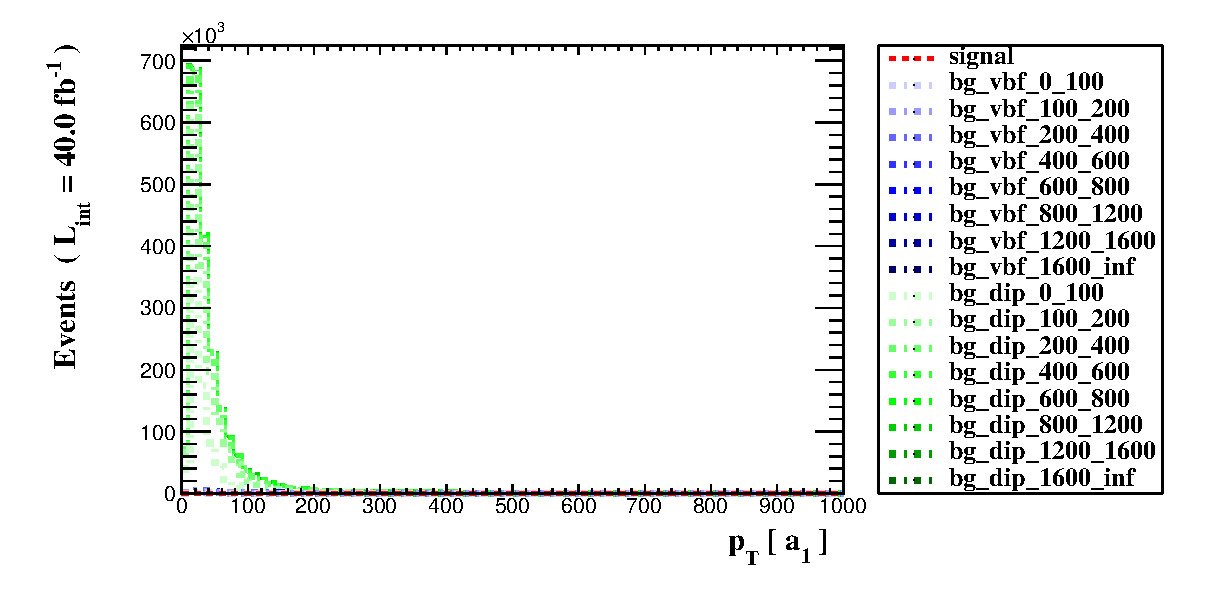
\includegraphics[scale=0.45]{selection_11.eps}\\
\caption{   }
  \end{center}
\end{figure}
      \newpage
\subsection{ Histogram 13}

\textbf{* Plot: PT ( a[2] ) }\\
   \begin{table}[H]
  \begin{center}
    \begin{tabular}{|m{23.0mm}|m{23.0mm}|m{18.0mm}|m{19.0mm}|m{19.0mm}|m{19.0mm}|m{19.0mm}|}
      \hline
      {\cellcolor{yellow}         Dataset}& {\cellcolor{yellow}         Integral}& {\cellcolor{yellow}         Entries per event}& {\cellcolor{yellow}         Mean}& {\cellcolor{yellow}         RMS}& {\cellcolor{yellow}         \% underflow}& {\cellcolor{yellow}         \% overflow}\\
      \hline
      {\cellcolor{white}         signal}& {\cellcolor{white}         4094}& {\cellcolor{white}         1.0}& {\cellcolor{white}         334.941}& {\cellcolor{white}         290.0}& {\cellcolor{green}         0.0}& {\cellcolor{green}         3.619}\\
      \hline
      {\cellcolor{white}         bg\_vbf\_0\_100}& {\cellcolor{white}         3934}& {\cellcolor{white}         1.0}& {\cellcolor{white}         18.2641}& {\cellcolor{white}         11.16}& {\cellcolor{green}         0.0}& {\cellcolor{green}         0.0}\\
      \hline
      {\cellcolor{white}         bg\_vbf\_100\_200}& {\cellcolor{white}         8756}& {\cellcolor{white}         1.0}& {\cellcolor{white}         21.2596}& {\cellcolor{white}         15.54}& {\cellcolor{green}         0.0}& {\cellcolor{green}         0.0}\\
      \hline
      {\cellcolor{white}         bg\_vbf\_200\_400}& {\cellcolor{white}         5358}& {\cellcolor{white}         1.0}& {\cellcolor{white}         25.9605}& {\cellcolor{white}         23.17}& {\cellcolor{green}         0.0}& {\cellcolor{green}         0.0002055}\\
      \hline
      {\cellcolor{white}         bg\_vbf\_400\_600}& {\cellcolor{white}         983}& {\cellcolor{white}         1.0}& {\cellcolor{white}         31.2333}& {\cellcolor{white}         32.38}& {\cellcolor{green}         0.0}& {\cellcolor{green}         0.0009032}\\
      \hline
      {\cellcolor{white}         bg\_vbf\_600\_800}& {\cellcolor{white}         251}& {\cellcolor{white}         1.0}& {\cellcolor{white}         34.5946}& {\cellcolor{white}         38.91}& {\cellcolor{green}         0.0}& {\cellcolor{green}         0.0001002}\\
      \hline
      {\cellcolor{white}         bg\_vbf\_800\_1200}& {\cellcolor{white}         114}& {\cellcolor{white}         1.0}& {\cellcolor{white}         37.1093}& {\cellcolor{white}         44.62}& {\cellcolor{green}         0.0}& {\cellcolor{green}         0.0009971}\\
      \hline
      {\cellcolor{white}         bg\_vbf\_1200\_1600}& {\cellcolor{white}         20.6}& {\cellcolor{white}         1.0}& {\cellcolor{white}         39.4356}& {\cellcolor{white}         49.91}& {\cellcolor{green}         0.0}& {\cellcolor{green}         0.002623}\\
      \hline
      {\cellcolor{white}         bg\_vbf\_1600\_inf}& {\cellcolor{white}         7.66}& {\cellcolor{white}         1.0}& {\cellcolor{white}         40.8098}& {\cellcolor{white}         52.8}& {\cellcolor{green}         0.0}& {\cellcolor{green}         0.004823}\\
      \hline
      {\cellcolor{white}         bg\_dip\_0\_100}& {\cellcolor{white}         714691}& {\cellcolor{white}         1.0}& {\cellcolor{white}         16.5201}& {\cellcolor{white}         9.637}& {\cellcolor{green}         0.0}& {\cellcolor{green}         0.0}\\
      \hline
      {\cellcolor{white}         bg\_dip\_100\_200}& {\cellcolor{white}         855479}& {\cellcolor{white}         1.0}& {\cellcolor{white}         18.8185}& {\cellcolor{white}         12.99}& {\cellcolor{green}         0.0}& {\cellcolor{green}         0.0}\\
      \hline
      {\cellcolor{white}         bg\_dip\_200\_400}& {\cellcolor{white}         234627}& {\cellcolor{white}         1.0}& {\cellcolor{white}         22.8735}& {\cellcolor{white}         19.58}& {\cellcolor{green}         0.0}& {\cellcolor{green}         0.0}\\
      \hline
      {\cellcolor{white}         bg\_dip\_400\_600}& {\cellcolor{white}         28616}& {\cellcolor{white}         1.0}& {\cellcolor{white}         26.8872}& {\cellcolor{white}         27.11}& {\cellcolor{green}         0.0}& {\cellcolor{green}         0.0001937}\\
      \hline
      {\cellcolor{white}         bg\_dip\_600\_800}& {\cellcolor{white}         6658}& {\cellcolor{white}         1.0}& {\cellcolor{white}         29.3925}& {\cellcolor{white}         32.02}& {\cellcolor{green}         0.0}& {\cellcolor{green}         0.0003031}\\
      \hline
      {\cellcolor{white}         bg\_dip\_800\_1200}& {\cellcolor{white}         2939}& {\cellcolor{white}         1.0}& {\cellcolor{white}         31.3973}& {\cellcolor{white}         35.97}& {\cellcolor{green}         0.0}& {\cellcolor{green}         0.0007697}\\
      \hline
      {\cellcolor{white}         bg\_dip\_1200\_1600}& {\cellcolor{white}         513}& {\cellcolor{white}         1.0}& {\cellcolor{white}         33.6461}& {\cellcolor{white}         39.79}& {\cellcolor{green}         0.0}& {\cellcolor{green}         0.001184}\\
      \hline
      {\cellcolor{white}         bg\_dip\_1600\_inf}& {\cellcolor{white}         187}& {\cellcolor{white}         1.0}& {\cellcolor{white}         35.6015}& {\cellcolor{white}         42.32}& {\cellcolor{green}         0.0}& {\cellcolor{green}         0.002116}\\
\hline
    \end{tabular}
  \end{center}
\end{table}

\begin{figure}[H]
  \begin{center}
    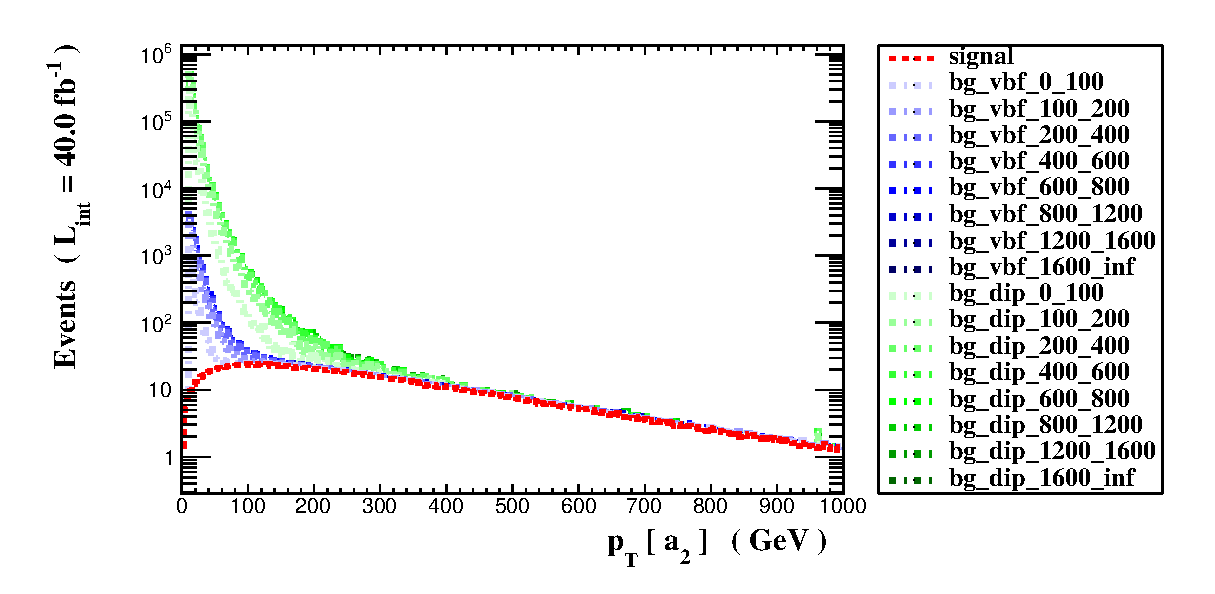
\includegraphics[scale=0.45]{selection_12.eps}\\
\caption{   }
  \end{center}
\end{figure}
      \newpage
\subsection{ Histogram 14}

\textbf{* Plot: THT}\\
   \begin{table}[H]
  \begin{center}
    \begin{tabular}{|m{23.0mm}|m{23.0mm}|m{18.0mm}|m{19.0mm}|m{19.0mm}|m{19.0mm}|m{19.0mm}|}
      \hline
      {\cellcolor{yellow}         Dataset}& {\cellcolor{yellow}         Integral}& {\cellcolor{yellow}         Entries per event}& {\cellcolor{yellow}         Mean}& {\cellcolor{yellow}         RMS}& {\cellcolor{yellow}         \% underflow}& {\cellcolor{yellow}         \% overflow}\\
      \hline
      {\cellcolor{white}         signal}& {\cellcolor{white}         4094}& {\cellcolor{white}         1.0}& {\cellcolor{white}         607.69}& {\cellcolor{white}         391.1}& {\cellcolor{red}         0.0}& {\cellcolor{red}         15.4}\\
      \hline
      {\cellcolor{white}         bg\_vbf\_0\_100}& {\cellcolor{white}         3934}& {\cellcolor{white}         1.0}& {\cellcolor{white}         78.0345}& {\cellcolor{white}         14.32}& {\cellcolor{green}         0.0}& {\cellcolor{green}         0.0}\\
      \hline
      {\cellcolor{white}         bg\_vbf\_100\_200}& {\cellcolor{white}         8756}& {\cellcolor{white}         1.0}& {\cellcolor{white}         144.593}& {\cellcolor{white}         27.95}& {\cellcolor{green}         0.0}& {\cellcolor{green}         0.0}\\
      \hline
      {\cellcolor{white}         bg\_vbf\_200\_400}& {\cellcolor{white}         5358}& {\cellcolor{white}         1.0}& {\cellcolor{white}         270.786}& {\cellcolor{white}         53.37}& {\cellcolor{green}         0.0}& {\cellcolor{green}         0.0}\\
      \hline
      {\cellcolor{white}         bg\_vbf\_400\_600}& {\cellcolor{white}         983}& {\cellcolor{white}         1.0}& {\cellcolor{white}         475.979}& {\cellcolor{white}         55.0}& {\cellcolor{green}         0.0}& {\cellcolor{green}         0.0}\\
      \hline
      {\cellcolor{white}         bg\_vbf\_600\_800}& {\cellcolor{white}         251}& {\cellcolor{white}         1.0}& {\cellcolor{white}         680.318}& {\cellcolor{white}         55.83}& {\cellcolor{green}         0.0}& {\cellcolor{green}         0.0}\\
      \hline
      {\cellcolor{white}         bg\_vbf\_800\_1200}& {\cellcolor{white}         114}& {\cellcolor{white}         1.0}& {\cellcolor{white}         939.672}& {\cellcolor{white}         106.7}& {\cellcolor{red}         0.0}& {\cellcolor{red}         27.89}\\
      \hline
      {\cellcolor{white}         bg\_vbf\_1200\_1600}& {\cellcolor{white}         20.6}& {\cellcolor{white}         1.0}& {\cellcolor{white}         1352.19}& {\cellcolor{white}         109.7}& {\cellcolor{red}         0.0}& {\cellcolor{red}         100.0}\\
      \hline
      {\cellcolor{white}         bg\_vbf\_1600\_inf}& {\cellcolor{white}         7.66}& {\cellcolor{white}         1.0}& {\cellcolor{white}         1966.54}& {\cellcolor{white}         391.6}& {\cellcolor{red}         0.0}& {\cellcolor{red}         100.0}\\
      \hline
      {\cellcolor{white}         bg\_dip\_0\_100}& {\cellcolor{white}         714691}& {\cellcolor{white}         1.0}& {\cellcolor{white}         74.1637}& {\cellcolor{white}         15.18}& {\cellcolor{green}         0.0}& {\cellcolor{green}         0.0}\\
      \hline
      {\cellcolor{white}         bg\_dip\_100\_200}& {\cellcolor{white}         855479}& {\cellcolor{white}         1.0}& {\cellcolor{white}         138.778}& {\cellcolor{white}         26.45}& {\cellcolor{green}         0.0}& {\cellcolor{green}         0.0}\\
      \hline
      {\cellcolor{white}         bg\_dip\_200\_400}& {\cellcolor{white}         234627}& {\cellcolor{white}         1.0}& {\cellcolor{white}         261.793}& {\cellcolor{white}         50.89}& {\cellcolor{green}         0.0}& {\cellcolor{green}         0.0}\\
      \hline
      {\cellcolor{white}         bg\_dip\_400\_600}& {\cellcolor{white}         28616}& {\cellcolor{white}         1.0}& {\cellcolor{white}         473.998}& {\cellcolor{white}         54.59}& {\cellcolor{green}         0.0}& {\cellcolor{green}         0.0}\\
      \hline
      {\cellcolor{white}         bg\_dip\_600\_800}& {\cellcolor{white}         6658}& {\cellcolor{white}         1.0}& {\cellcolor{white}         679.873}& {\cellcolor{white}         55.79}& {\cellcolor{green}         0.0}& {\cellcolor{green}         0.0}\\
      \hline
      {\cellcolor{white}         bg\_dip\_800\_1200}& {\cellcolor{white}         2939}& {\cellcolor{white}         1.0}& {\cellcolor{white}         939.623}& {\cellcolor{white}         106.7}& {\cellcolor{red}         0.0}& {\cellcolor{red}         27.8}\\
      \hline
      {\cellcolor{white}         bg\_dip\_1200\_1600}& {\cellcolor{white}         513}& {\cellcolor{white}         1.0}& {\cellcolor{white}         1352.11}& {\cellcolor{white}         109.8}& {\cellcolor{red}         0.0}& {\cellcolor{red}         100.0}\\
      \hline
      {\cellcolor{white}         bg\_dip\_1600\_inf}& {\cellcolor{white}         187}& {\cellcolor{white}         1.0}& {\cellcolor{white}         1962.59}& {\cellcolor{white}         386.0}& {\cellcolor{red}         0.0}& {\cellcolor{red}         100.0}\\
\hline
    \end{tabular}
  \end{center}
\end{table}

\begin{figure}[H]
  \begin{center}
    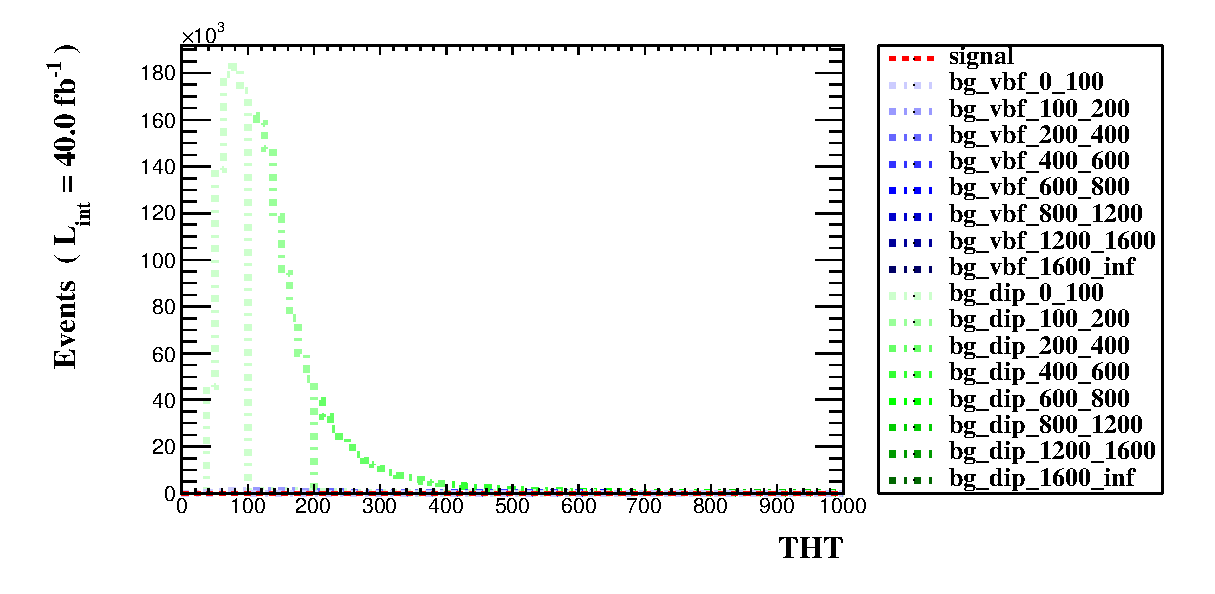
\includegraphics[scale=0.45]{selection_13.eps}\\
\caption{   }
  \end{center}
\end{figure}
      \newpage
\subsection{ Histogram 15}

\textbf{* Plot: MET}\\
   \begin{table}[H]
  \begin{center}
    \begin{tabular}{|m{23.0mm}|m{23.0mm}|m{18.0mm}|m{19.0mm}|m{19.0mm}|m{19.0mm}|m{19.0mm}|}
      \hline
      {\cellcolor{yellow}         Dataset}& {\cellcolor{yellow}         Integral}& {\cellcolor{yellow}         Entries per event}& {\cellcolor{yellow}         Mean}& {\cellcolor{yellow}         RMS}& {\cellcolor{yellow}         \% underflow}& {\cellcolor{yellow}         \% overflow}\\
      \hline
      {\cellcolor{white}         signal}& {\cellcolor{white}         4094}& {\cellcolor{white}         1.0}& {\cellcolor{white}         8.33083e-09}& {\cellcolor{white}         1.078e-08}& {\cellcolor{green}         0.0}& {\cellcolor{green}         0.0}\\
      \hline
      {\cellcolor{white}         bg\_vbf\_0\_100}& {\cellcolor{white}         3934}& {\cellcolor{white}         1.0}& {\cellcolor{white}         5.97855e-10}& {\cellcolor{white}         4.233e-10}& {\cellcolor{green}         0.0}& {\cellcolor{green}         0.0}\\
      \hline
      {\cellcolor{white}         bg\_vbf\_100\_200}& {\cellcolor{white}         8756}& {\cellcolor{white}         1.0}& {\cellcolor{white}         9.55638e-10}& {\cellcolor{white}         1.098e-09}& {\cellcolor{green}         0.0}& {\cellcolor{green}         0.0}\\
      \hline
      {\cellcolor{white}         bg\_vbf\_200\_400}& {\cellcolor{white}         5358}& {\cellcolor{white}         1.0}& {\cellcolor{white}         3.23057e-09}& {\cellcolor{white}         2.219e-09}& {\cellcolor{green}         0.0}& {\cellcolor{green}         0.0}\\
      \hline
      {\cellcolor{white}         bg\_vbf\_400\_600}& {\cellcolor{white}         983}& {\cellcolor{white}         1.0}& {\cellcolor{white}         4.52485e-09}& {\cellcolor{white}         2.611e-09}& {\cellcolor{green}         0.0}& {\cellcolor{green}         0.0}\\
      \hline
      {\cellcolor{white}         bg\_vbf\_600\_800}& {\cellcolor{white}         251}& {\cellcolor{white}         1.0}& {\cellcolor{white}         4.90226e-09}& {\cellcolor{white}         2.72e-09}& {\cellcolor{green}         0.0}& {\cellcolor{green}         0.0}\\
      \hline
      {\cellcolor{white}         bg\_vbf\_800\_1200}& {\cellcolor{white}         114}& {\cellcolor{white}         1.0}& {\cellcolor{white}         5.15622e-09}& {\cellcolor{white}         2.979e-09}& {\cellcolor{green}         0.0}& {\cellcolor{green}         0.0}\\
      \hline
      {\cellcolor{white}         bg\_vbf\_1200\_1600}& {\cellcolor{white}         20.6}& {\cellcolor{white}         1.0}& {\cellcolor{white}         5.81971e-09}& {\cellcolor{white}         5.339e-09}& {\cellcolor{green}         0.0}& {\cellcolor{green}         0.0}\\
      \hline
      {\cellcolor{white}         bg\_vbf\_1600\_inf}& {\cellcolor{white}         7.66}& {\cellcolor{white}         1.0}& {\cellcolor{white}         1.30635e-08}& {\cellcolor{white}         1.639e-08}& {\cellcolor{green}         0.0}& {\cellcolor{green}         0.0}\\
      \hline
      {\cellcolor{white}         bg\_dip\_0\_100}& {\cellcolor{white}         714691}& {\cellcolor{white}         1.0}& {\cellcolor{white}         5.87329e-10}& {\cellcolor{white}         4.134e-10}& {\cellcolor{green}         0.0}& {\cellcolor{green}         0.0}\\
      \hline
      {\cellcolor{white}         bg\_dip\_100\_200}& {\cellcolor{white}         855479}& {\cellcolor{white}         1.0}& {\cellcolor{white}         8.95295e-10}& {\cellcolor{white}         1.036e-09}& {\cellcolor{green}         0.0}& {\cellcolor{green}         0.0}\\
      \hline
      {\cellcolor{white}         bg\_dip\_200\_400}& {\cellcolor{white}         234627}& {\cellcolor{white}         1.0}& {\cellcolor{white}         3.11256e-09}& {\cellcolor{white}         2.186e-09}& {\cellcolor{green}         0.0}& {\cellcolor{green}         0.0}\\
      \hline
      {\cellcolor{white}         bg\_dip\_400\_600}& {\cellcolor{white}         28616}& {\cellcolor{white}         1.0}& {\cellcolor{white}         4.43451e-09}& {\cellcolor{white}         2.58e-09}& {\cellcolor{green}         0.0}& {\cellcolor{green}         0.0}\\
      \hline
      {\cellcolor{white}         bg\_dip\_600\_800}& {\cellcolor{white}         6658}& {\cellcolor{white}         1.0}& {\cellcolor{white}         4.80208e-09}& {\cellcolor{white}         2.678e-09}& {\cellcolor{green}         0.0}& {\cellcolor{green}         0.0}\\
      \hline
      {\cellcolor{white}         bg\_dip\_800\_1200}& {\cellcolor{white}         2939}& {\cellcolor{white}         1.0}& {\cellcolor{white}         5.06231e-09}& {\cellcolor{white}         3.026e-09}& {\cellcolor{green}         0.0}& {\cellcolor{green}         0.0}\\
      \hline
      {\cellcolor{white}         bg\_dip\_1200\_1600}& {\cellcolor{white}         513}& {\cellcolor{white}         1.0}& {\cellcolor{white}         5.58908e-09}& {\cellcolor{white}         4.823e-09}& {\cellcolor{green}         0.0}& {\cellcolor{green}         0.0}\\
      \hline
      {\cellcolor{white}         bg\_dip\_1600\_inf}& {\cellcolor{white}         187}& {\cellcolor{white}         1.0}& {\cellcolor{white}         1.25075e-08}& {\cellcolor{white}         1.605e-08}& {\cellcolor{green}         0.0}& {\cellcolor{green}         0.0}\\
\hline
    \end{tabular}
  \end{center}
\end{table}

\begin{figure}[H]
  \begin{center}
    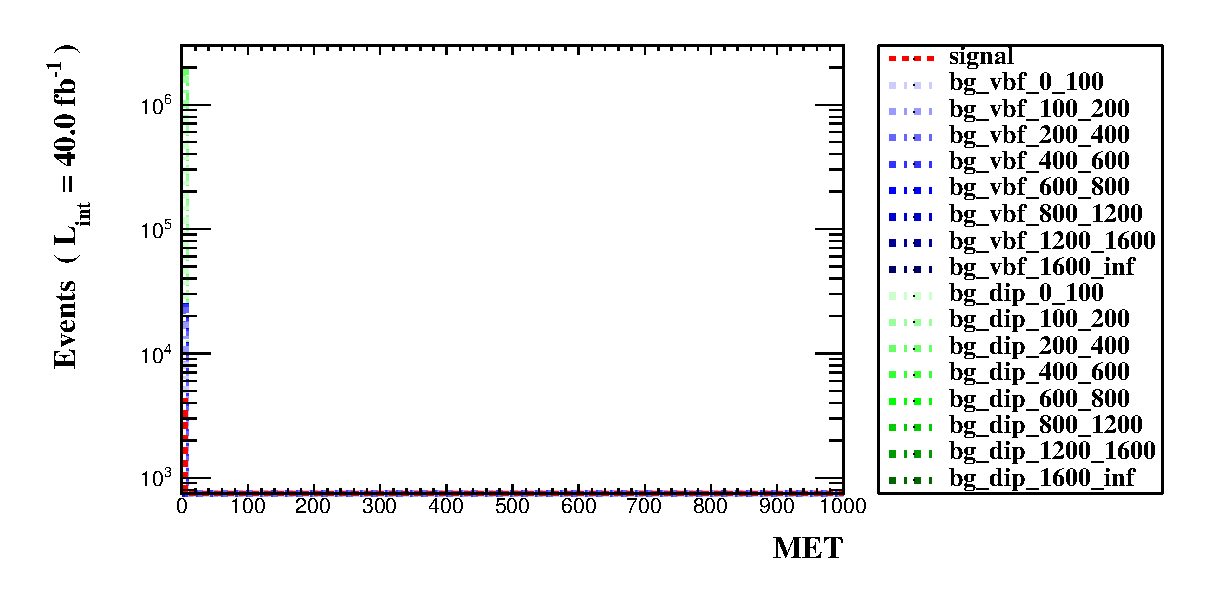
\includegraphics[scale=0.45]{selection_14.eps}\\
\caption{   }
  \end{center}
\end{figure}
      \newpage
\subsection{ Histogram 16}

\textbf{* Plot: TET}\\
   \begin{table}[H]
  \begin{center}
    \begin{tabular}{|m{23.0mm}|m{23.0mm}|m{18.0mm}|m{19.0mm}|m{19.0mm}|m{19.0mm}|m{19.0mm}|}
      \hline
      {\cellcolor{yellow}         Dataset}& {\cellcolor{yellow}         Integral}& {\cellcolor{yellow}         Entries per event}& {\cellcolor{yellow}         Mean}& {\cellcolor{yellow}         RMS}& {\cellcolor{yellow}         \% underflow}& {\cellcolor{yellow}         \% overflow}\\
      \hline
      {\cellcolor{white}         signal}& {\cellcolor{white}         4094}& {\cellcolor{white}         1.0}& {\cellcolor{white}         1530.72}& {\cellcolor{white}         825.3}& {\cellcolor{red}         0.0}& {\cellcolor{red}         70.59}\\
      \hline
      {\cellcolor{white}         bg\_vbf\_0\_100}& {\cellcolor{white}         3934}& {\cellcolor{white}         1.0}& {\cellcolor{white}         129.338}& {\cellcolor{white}         32.52}& {\cellcolor{green}         0.0}& {\cellcolor{green}         0.001235}\\
      \hline
      {\cellcolor{white}         bg\_vbf\_100\_200}& {\cellcolor{white}         8756}& {\cellcolor{white}         1.0}& {\cellcolor{white}         212.346}& {\cellcolor{white}         54.5}& {\cellcolor{green}         0.0}& {\cellcolor{green}         0.00344}\\
      \hline
      {\cellcolor{white}         bg\_vbf\_200\_400}& {\cellcolor{white}         5358}& {\cellcolor{white}         1.0}& {\cellcolor{white}         368.751}& {\cellcolor{white}         98.32}& {\cellcolor{green}         0.0}& {\cellcolor{green}         0.04948}\\
      \hline
      {\cellcolor{white}         bg\_vbf\_400\_600}& {\cellcolor{white}         983}& {\cellcolor{white}         1.0}& {\cellcolor{white}         614.098}& {\cellcolor{white}         136.7}& {\cellcolor{green}         0.0}& {\cellcolor{green}         1.955}\\
      \hline
      {\cellcolor{white}         bg\_vbf\_600\_800}& {\cellcolor{white}         251}& {\cellcolor{white}         1.0}& {\cellcolor{white}         847.293}& {\cellcolor{white}         172.9}& {\cellcolor{red}         0.0}& {\cellcolor{red}         15.03}\\
      \hline
      {\cellcolor{white}         bg\_vbf\_800\_1200}& {\cellcolor{white}         114}& {\cellcolor{white}         1.0}& {\cellcolor{white}         1130.93}& {\cellcolor{white}         233.4}& {\cellcolor{red}         0.0}& {\cellcolor{red}         66.91}\\
      \hline
      {\cellcolor{white}         bg\_vbf\_1200\_1600}& {\cellcolor{white}         20.6}& {\cellcolor{white}         1.0}& {\cellcolor{white}         1564.51}& {\cellcolor{white}         271.2}& {\cellcolor{red}         0.0}& {\cellcolor{red}         100.0}\\
      \hline
      {\cellcolor{white}         bg\_vbf\_1600\_inf}& {\cellcolor{white}         7.66}& {\cellcolor{white}         1.0}& {\cellcolor{white}         2188.52}& {\cellcolor{white}         475.9}& {\cellcolor{red}         0.0}& {\cellcolor{red}         100.0}\\
      \hline
      {\cellcolor{white}         bg\_dip\_0\_100}& {\cellcolor{white}         714691}& {\cellcolor{white}         1.0}& {\cellcolor{white}         120.486}& {\cellcolor{white}         31.72}& {\cellcolor{green}         0.0}& {\cellcolor{green}         0.0}\\
      \hline
      {\cellcolor{white}         bg\_dip\_100\_200}& {\cellcolor{white}         855479}& {\cellcolor{white}         1.0}& {\cellcolor{white}         199.807}& {\cellcolor{white}         52.08}& {\cellcolor{green}         0.0}& {\cellcolor{green}         0.0009859}\\
      \hline
      {\cellcolor{white}         bg\_dip\_200\_400}& {\cellcolor{white}         234627}& {\cellcolor{white}         1.0}& {\cellcolor{white}         351.793}& {\cellcolor{white}         94.87}& {\cellcolor{green}         0.0}& {\cellcolor{green}         0.02749}\\
      \hline
      {\cellcolor{white}         bg\_dip\_400\_600}& {\cellcolor{white}         28616}& {\cellcolor{white}         1.0}& {\cellcolor{white}         596.305}& {\cellcolor{white}         134.8}& {\cellcolor{green}         0.0}& {\cellcolor{green}         1.993}\\
      \hline
      {\cellcolor{white}         bg\_dip\_600\_800}& {\cellcolor{white}         6658}& {\cellcolor{white}         1.0}& {\cellcolor{white}         822.647}& {\cellcolor{white}         165.9}& {\cellcolor{orange}         0.0}& {\cellcolor{orange}         10.92}\\
      \hline
      {\cellcolor{white}         bg\_dip\_800\_1200}& {\cellcolor{white}         2939}& {\cellcolor{white}         1.0}& {\cellcolor{white}         1097.74}& {\cellcolor{white}         215.8}& {\cellcolor{red}         0.0}& {\cellcolor{red}         61.64}\\
      \hline
      {\cellcolor{white}         bg\_dip\_1200\_1600}& {\cellcolor{white}         513}& {\cellcolor{white}         1.0}& {\cellcolor{white}         1524.46}& {\cellcolor{white}         238.7}& {\cellcolor{red}         0.0}& {\cellcolor{red}         100.0}\\
      \hline
      {\cellcolor{white}         bg\_dip\_1600\_inf}& {\cellcolor{white}         187}& {\cellcolor{white}         1.0}& {\cellcolor{white}         2144.43}& {\cellcolor{white}         445.2}& {\cellcolor{red}         0.0}& {\cellcolor{red}         100.0}\\
\hline
    \end{tabular}
  \end{center}
\end{table}

\begin{figure}[H]
  \begin{center}
    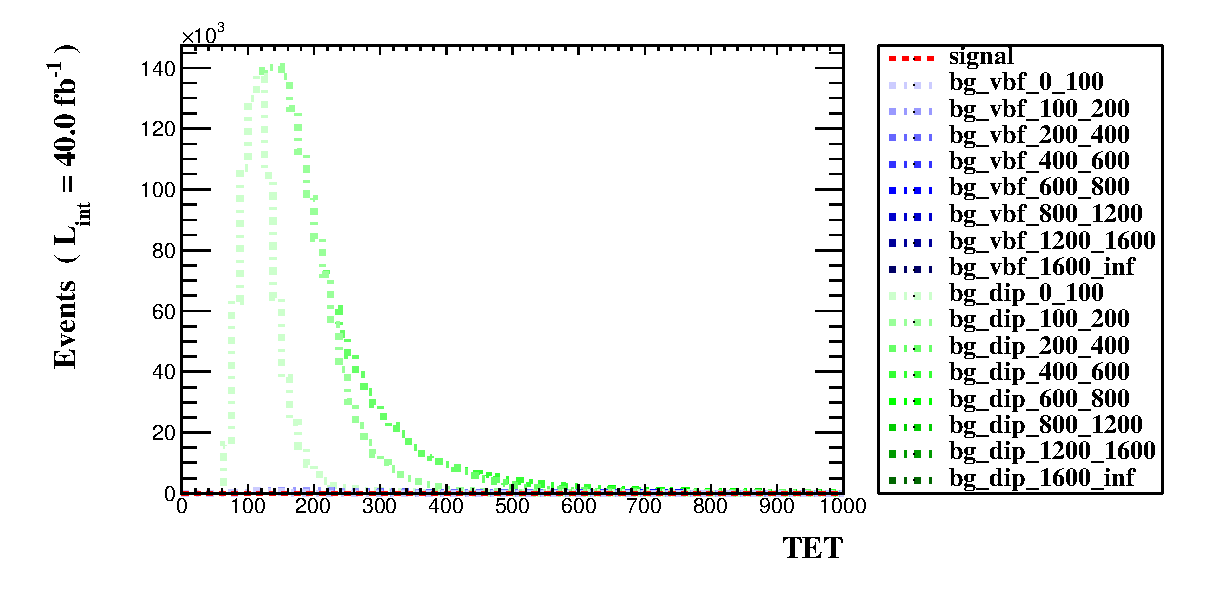
\includegraphics[scale=0.45]{selection_15.eps}\\
\caption{   }
  \end{center}
\end{figure}
      \newpage
\subsection{Cut 2}

\textbf{* Cut: select ( sdETA ( jets[1] jets[2] ) > 3.6 or sdETA ( jets[1] jets[2] ) < -3.6 ) and M ( jets[1] jets[2] ) > 750.0}\\
   \begin{table}[H]
  \begin{center}
    \begin{tabular}{|m{20.0mm}|m{27.0mm}|m{27.0mm}|m{33.0mm}|m{32.0mm}|}
      \hline
      {\cellcolor{yellow}         Dataset}& {\cellcolor{yellow}         Events kept:
          K}& {\cellcolor{yellow}         Rejected events:
          R}& {\cellcolor{yellow}         Efficiency:
          K /\- (K + R)}& {\cellcolor{yellow}         Cumul. efficiency:
          K /\- Initial}\\
      \hline
      {\cellcolor{white}         signal}& {\cellcolor{white}         1195.7 +/\-- 29.1}& {\cellcolor{white}         2898.4 +/\-- 29.1}& {\cellcolor{white}         0.29205 +/\-- 0.00711}& {\cellcolor{white}         0.29205 +/\-- 0.00711}\\
      \hline
      {\cellcolor{white}         bg\_vbf\_0\_100}& {\cellcolor{white}         658.8 +/\-- 25.0}& {\cellcolor{white}         3275.9 +/\-- 49.3}& {\cellcolor{white}         0.16744 +/\-- 0.00595}& {\cellcolor{white}         0.05422 +/\-- 0.00205}\\
      \hline
      {\cellcolor{white}         bg\_vbf\_100\_200}& {\cellcolor{white}         2348.1 +/\-- 42.4}& {\cellcolor{white}         6408.9 +/\-- 47.9}& {\cellcolor{white}         0.26814 +/\-- 0.00473}& {\cellcolor{white}         0.24219 +/\-- 0.00435}\\
      \hline
      {\cellcolor{white}         bg\_vbf\_200\_400}& {\cellcolor{white}         2048.2 +/\-- 35.9}& {\cellcolor{white}         3310.5 +/\-- 36.5}& {\cellcolor{white}         0.38222 +/\-- 0.00664}& {\cellcolor{white}         0.37838 +/\-- 0.00659}\\
      \hline
      {\cellcolor{white}         bg\_vbf\_400\_600}& {\cellcolor{white}         280.0 +/\-- 14.2}& {\cellcolor{white}         703.8 +/\-- 14.2}& {\cellcolor{white}         0.2846 +/\-- 0.0144}& {\cellcolor{white}         0.2837 +/\-- 0.0144}\\
      \hline
      {\cellcolor{white}         bg\_vbf\_600\_800}& {\cellcolor{white}         48.00 +/\-- 6.23}& {\cellcolor{white}         203.85 +/\-- 6.25}& {\cellcolor{white}         0.1906 +/\-- 0.0247}& {\cellcolor{white}         0.1904 +/\-- 0.0247}\\
      \hline
      {\cellcolor{white}         bg\_vbf\_800\_1200}& {\cellcolor{white}         12.08 +/\-- 3.29}& {\cellcolor{white}         102.56 +/\-- 3.31}& {\cellcolor{white}         0.1054 +/\-- 0.0287}& {\cellcolor{white}         0.1053 +/\-- 0.0287}\\
      \hline
      {\cellcolor{white}         bg\_vbf\_1200\_1600}& {\cellcolor{white}         0.678 +/\-- 0.810}& {\cellcolor{white}         19.875 +/\-- 0.835}& {\cellcolor{white}         0.033 +/\-- 0.039}& {\cellcolor{white}         0.0329 +/\-- 0.0393}\\
      \hline
      {\cellcolor{white}         bg\_vbf\_1600\_inf}& {\cellcolor{white}         0.0483 +/\-- 0.2191}& {\cellcolor{white}         7.465 +/\-- 0.435}& {\cellcolor{white}         0.00643 +/\-- 0.02916}& {\cellcolor{white}         0.00631 +/\-- 0.02860}\\
      \hline
      {\cellcolor{white}         bg\_dip\_0\_100}& {\cellcolor{white}         3323.2 +/\-- 57.9}& {\cellcolor{white}         711369 +/\-- 1410}& {\cellcolor{white}         4.65e-03 +/\-- 8.05e-05}& {\cellcolor{white}         1.23e-03 +/\-- 2.13e-05}\\
      \hline
      {\cellcolor{white}         bg\_dip\_100\_200}& {\cellcolor{white}         8614.4 +/\-- 93.2}& {\cellcolor{white}         846865 +/\-- 1259}& {\cellcolor{white}         0.010070 +/\-- 0.000108}& {\cellcolor{white}         7.86e-03 +/\-- 8.44e-05}\\
      \hline
      {\cellcolor{white}         bg\_dip\_200\_400}& {\cellcolor{white}         7092.8 +/\-- 83.9}& {\cellcolor{white}         227535 +/\-- 407}& {\cellcolor{white}         0.030230 +/\-- 0.000353}& {\cellcolor{white}         0.029609 +/\-- 0.000346}\\
      \hline
      {\cellcolor{white}         bg\_dip\_400\_600}& {\cellcolor{white}         658.2 +/\-- 25.4}& {\cellcolor{white}         27958.0 +/\-- 58.2}& {\cellcolor{white}         0.023001 +/\-- 0.000886}& {\cellcolor{white}         0.022856 +/\-- 0.000881}\\
      \hline
      {\cellcolor{white}         bg\_dip\_600\_800}& {\cellcolor{white}         93.79 +/\-- 9.62}& {\cellcolor{white}         6565.1 +/\-- 29.1}& {\cellcolor{white}         0.01409 +/\-- 0.00144}& {\cellcolor{white}         0.01405 +/\-- 0.00144}\\
      \hline
      {\cellcolor{white}         bg\_dip\_800\_1200}& {\cellcolor{white}         22.89 +/\-- 4.77}& {\cellcolor{white}         2917.07 +/\-- 7.08}& {\cellcolor{white}         0.00779 +/\-- 0.00162}& {\cellcolor{white}         0.00778 +/\-- 0.00162}\\
      \hline
      {\cellcolor{white}         bg\_dip\_1200\_1600}& {\cellcolor{white}         1.36 +/\-- 1.17}& {\cellcolor{white}         512.0 +/\-- 2.9}& {\cellcolor{white}         0.00265 +/\-- 0.00227}& {\cellcolor{white}         0.00265 +/\-- 0.00227}\\
      \hline
      {\cellcolor{white}         bg\_dip\_1600\_inf}& {\cellcolor{white}         0.0932 +/\-- 0.3051}& {\cellcolor{white}         187.65 +/\-- 0.46}& {\cellcolor{white}         0.000496 +/\-- 0.001625}& {\cellcolor{white}         0.000496 +/\-- 0.001625}\\
\hline
    \end{tabular}
  \end{center}
\end{table}

   % -----------------------------------------------------------------------------
%                                SECTION Summary                                
% -----------------------------------------------------------------------------
\newpage
\section{ Summary}

\subsection{Cut-flow charts}

\begin{itemize}
  \item How to compare signal (S) and background (B): \textcolor{blue}{S/\-sqrt(S+B)} .
   \item Object definition selections are indicated in cyan.  \item Reject and select are indicated by 'REJ' and 'SEL' respectively
\end{itemize}
\begin{table}[H]
  \begin{center}
    \begin{tabular}{|m{36.0mm}|m{36.0mm}|m{36.0mm}|m{33.0mm}|}
      \hline
      {\cellcolor{yellow}        Cuts}& {\cellcolor{yellow}         Signal (S)}& {\cellcolor{yellow}         Background (B)}& {\cellcolor{yellow}         S vs B}\\
      \hline
      {\cellcolor{white}         Initial (no cut)}& {\cellcolor{white}         4094.08 +/\-- 1.13}& {\cellcolor{white}         4113516 +/\-- 4877}& {\cellcolor{white}         2.01760 +/\-- 0.00132}\\
      \hline
      {\cellcolor{white} SEL: M ( jets[1] jets[2] ) > 120.0}& {\cellcolor{white}         4094.04 +/\-- 1.14}& {\cellcolor{white}         1863145 +/\-- 1947}& {\cellcolor{white}         2.99607 +/\-- 0.00177}\\
      \hline
      {\cellcolor{white} SEL: ( sdETA ( jets[1] jets[2] ) > 3.6 or sdETA ( }& {\cellcolor{white}         1195.7 +/\-- 29.1}& {\cellcolor{white}         25202 +/\-- 154}& {\cellcolor{white}         7.359 +/\-- 0.176}\\
\hline
    \end{tabular}
  \end{center}
\end{table}

\end{document}
